\documentclass{book}

\usepackage{float}
\usepackage{amsmath}
\usepackage{amsfonts}
\usepackage{graphicx}
\usepackage{lineno}
\usepackage{natbib}
\usepackage[pdfpagemode=UseNone, pdfstartview=FitH]{hyperref}
\usepackage{verbatim}
\usepackage{soul}
\usepackage{color}
%\usepackage{fancyvrb}
\usepackage{textcomp}
\usepackage{bm}

\bibliographystyle{asa}

\floatstyle{plain}
\floatname{panel}{Panel}
\newfloat{algorithm}{h}{txt}[chapter]
\newfloat{panel}{h}{txt}[chapter]


\newcommand{\R}{\textbf{R}}
\newcommand{\bugs}{\textbf{BUGS}}
\newcommand{\jags}{\textbf{JAGS}}
\newcommand{\secr}{\mbox{\tt secr}}
\newcommand{\scrbook}{\mbox{\tt scrbook}}
\newcommand{\mytilde}{$\sim$}


\linenumbers

\begin{document}

%\chapter{
%Modeling Animal space-usage with
%Detection Models based on Ecological Distance
%Ecological Distance Models in Spatial Capture-Recapture
Modeling Landscape Connectivity
}
\markboth{Ecological Distance}{}
\label{chapt.ecoldist}


\vspace{.3in}


Every spatial capture-recapture model that we have considered so far
has expressed encounter probability as function of the Euclidean
distance between individual activity centers ${\bf s}$ and trap
locations ${\bf x}$.  As a practical matter, models based on Euclidean
distance imply circular, symmetric, and stationary home ranges of
individuals, and these are not often biologically realistic.  While
these simple encounter probability models will often be sufficient for
practical purposes, especially in small data sets, sometimes
developing more complex models of the detection process as it relates
to space usage of individuals will be useful.  Animals may not judge
distance in terms of Euclidean distance but, rather, according to
the configuration of habitat patches, quality of local habitat, %landscape connectivity,
perceived mortality
risk, and other considerations. % affecting movement behavior.
Together, the degree to which these factors facilitate or impede
movement determines landscape connectivity
\citep{tischendorf_fahrig:2000}, which is widely recognized to be an
important component of population viability
\citep{with_crist:1995,compton_etal:2007}.
Moreover, because encounter probability and the distance metric upon which it is
based represent outcomes of individual movements about their home
range, ecologists might have explicit hypotheses about how
environmental variables affect the distance metric, and it is
therefore desirable to incorporate these hypotheses directly into SCR
models so that they may be formally evaluated statistically.

%Assessing the impacts of habitat fragmentation and habitat loss on
%population density and landscape connectivity are high priorities in
%applied ecological research.  %Landscape connectivity is defined as the
%degree to which landscape structure impedes or facilitates movement
%\citep{tischendorf_fahrig:2000} and is widely recognized to be an
%important component of population viability
%\citep{with_crist:1995}.
Although much theory has been developed to
predict the effects of decreasing connectivity, few empirical studies
have been conducted to test these predictions due to the paucity of
formal methods for estimating connectivity parameters
\citep{cushman_etal:2010}. Instead, ecologists often rely on expert
opinion or \textit{ad hoc} methods of specifying connectivity values,
even in important applied settings
\citep{adriaensen_etal:2003,beier_etal:2008,zeller_etal:2012}. In
addition, no methods are available for simultaneously estimating
population density and connectivity parameters, in spite of theory
predicting interacting effects of density and connectivity on
population viability \citep{tischendorf_etal:2005,cushman_etal:2010}.
In this chapter, following \citet{royle_etal:2012ecol}, we provide a
framework for modeling landscape connectivity using SCR models, by
parameterizing models for encounter probability based on ``ecological
distance''.  A natural candidate framework for modeling ecological
distance is the least-cost path which is used widely in landscape
ecology for modeling connectivity, movement and gene flow
\citep{adriaensen_etal:2003,manel_etal:2003,mcrae_etal:2008}.  In
practical applications, variables that influence landscape
connectivity, or the effective cost of moving across the landscape,
include things like highways \citep[e.g.,][]{epps_etal:2005},
elevation \citep{cushman_etal:2006}, ruggedness
\citep{epps_etal:2007}, snow cover \citep{schwartz_etal:2009},
distance to escape terrain \citep{shirk_etal:2010}, range limitations
\citep{mcrae_beier:2007}, or distance from urban areas, highways,
human disturbance or other factors that animals might avoid.


\citet{royle_etal:2012ecol} provided an SCR
framework based on least-cost path for modeling landscape
connectivity. They parameterized encounter probability
based not on Euclidean distance but, rather,
on the least-cost path between an individual's activity center and a
trap location. This is parameterized in terms of one or more
parameters that relate the {\it resistance} of the landscape to
explicit covariates.  In this way, SCR models can explicitly accommodate
landscape structure and account for connectivity of the landscape.
%For these models based on least-cost path, it is convenient to use a
%likelihood-based inference framework which we follow here in this
%chapter.
Using this
methodological extension of SCR models, it is possible to make formal
statistical inferences about movement and connectivity from
capture-recapture studies that generate sparse individual encounter
history data without subjective prescription of resistance or cost
surfaces. %, which is commonly done in practice. XXXX already said
While we believe there
should be much ecological interest in developing SCR models that
account for landscape connectivity, it is also important for obtaining
more accurate estimates of density; under simple models of landscape
connectivity, incorrectly fitting the basic model SCR0 produces
substantial bias in estimates of $N$ and hence density  \citep{royle_etal:2012ecol}.


\section{Shortcomings of Euclidean Distance Models}

In the standard SCR models, encounter probability is modeled as a
function of Euclidean distance. For example, using the binomial
observation model (Chapt. \ref{chapt.scr0}), let $y_{ij}$ be
individual- and trap-specific binomial counts with sample size $K$ and
probabilities $p_{ij}$. The Gaussian model is
\[
p_{ij} = p_{0} \exp(-  d_{ij}^2 /(2\sigma^{2}) )
\]
where $d_{ij} = ||{\bf x}_{j} - {\bf s}_{i}||$ is Euclidean
distance. As usual, we will sometimes adopt the log-scale
parameterization based on $\log(p_{ij})= \alpha_{0} + \alpha_{1}
d_{ij}^{2}$ where where $\alpha_{0} = \log(p_{0})$ and $\alpha_{1} =
-1/(2\sigma^2)$.

The main problem with the Euclidean distance metric in this encounter
probability model is that it is unaffected by habitat or landscape
structure, and it implies that the space used by individuals is
stationary and symmetric, which may be unreasonable assumptions for
some species. By stationary %here
we mean in the formal sense of
invariance to translation. That is, the properties of an individual
home range centered at some point ${\bf s}$ are exactly the same as
any other point say ${\bf s}'$.  As an example, if the common
detection model based on a bivariate normal probability distribution
function is used, then the implied space usage by {\it all}
individuals, no matter their location in space or local habitat
conditions, is symmetric with circular contours of usage intensity.

In the framework of \citet{royle_etal:2012ecol}, SCR models explicitly
incorporate information about the landscape so that a unit of distance
is variable depending on identified covariates, say
$C({\bf x})$. %$z({\bf x})$.
Thus, where an individual lives on the landscape, and the state of the
surrounding landscape, will determine the character of its usage of
space. In particular, they suggest distance metrics, based on
least-cost path, that imply irregular, asymmetric and non-stationary
home ranges of individuals. As an example, Fig. \ref{fig.distort}
shows a typical symmetric home range (left panel), and a compressed
home range (right panel) resulting from the effect of an environmental
variable (center panel) on an animal's movement behavior. We might
think of the environmental variable as representing an elevation
gradient of a valley and so, for a species that avoids high elevation,
space usage will be concentrated in flatter terrain at lower
elevations and therefore producing the elliptical home range shape.
%We reproduce the application from \citet{royle_etal:2012ecol} later in
%this chapter, in addition to providing an alternative applied context
%that involves computing distances within odd-shaped landscape patches
%(Sec. \ref{ecoldist.sec.buffer}).


\begin{figure}[h]
\centering
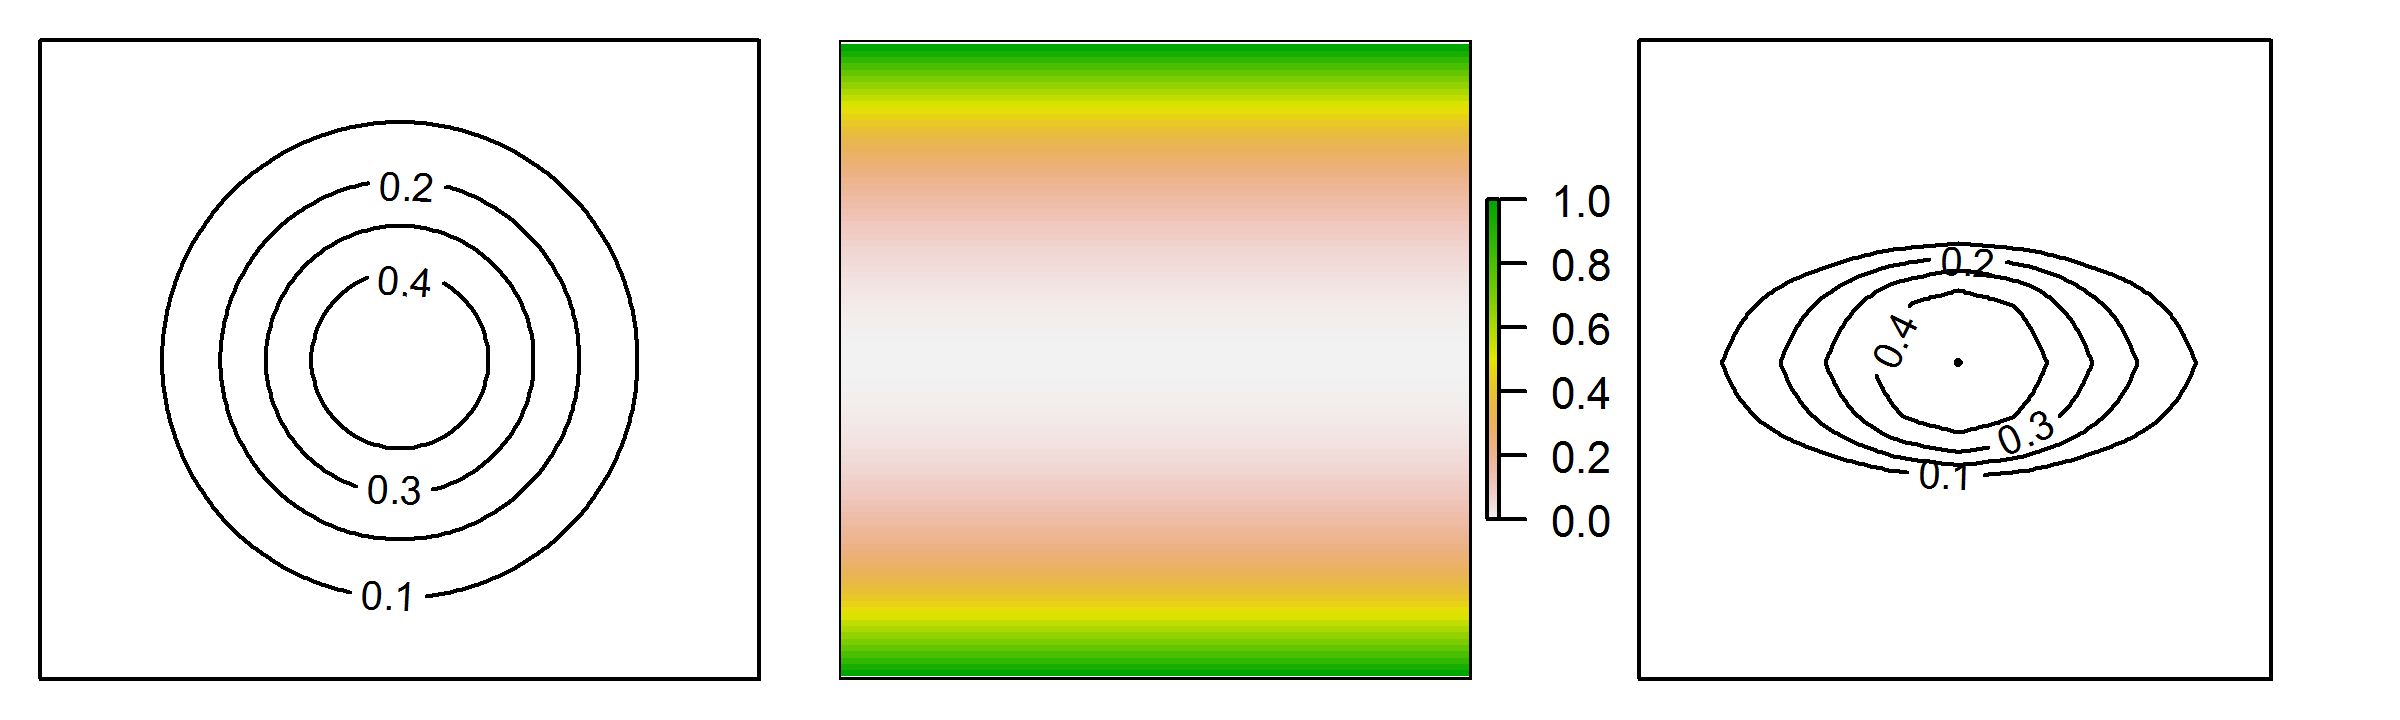
\includegraphics[width=5in,height=1.3in]{Ch12-EcolDist/figs/distort}
\caption{A symmetric home range (left), a habitat variable (center)
  such as representing an elevation gradient,
  and a non-symmetric home range (right) resulting from the cost imposed on
  movement by the habitat variable.}
\label{fig.distort}
\end{figure}


\section{Least-Cost Path Distance}

We adopt a cost-weighted distance metric here which defines the
effective distance between points by accumulating pixel-specific costs
determined using a cost function defined by the user.  The idea of
cost-weighted distance to characterize animal use of landscapes is
widely used in landscape ecology for modeling connectivity, movement
and gene flow \citep{beier_etal:2008}. For reasons of computational
tractability we consider a discrete landscape defined by a raster of
some prescribed resolution. The distance between any two points ${\bf
  x}$ and ${\bf x}'$ can be represented by a sequence of line segments
connecting neighboring pixels, say ${\bf l}_{1},{\bf
  l}_{2},\ldots,{\bf l}_{m}$. Then the cost-weighted distance between
${\bf x}$ and ${\bf x}'$ is
\begin{equation}
 d({\bf x},{\bf x}')
  =  \sum_{i=1}^{m-1} \mbox{cost}({\bf l}_{i},{\bf l}_{i+1})||{\bf l}_{i} - {\bf l}_{i+1}||
\label{eq.costweighted}
\end{equation}
where $\mbox{cost}({\bf l}_{i},{\bf l}_{i+1})$ is the user-defined cost to
move from pixel ${\bf l}_{i}$ to neighboring pixel ${\bf l}_{i+1}$ in
the sequence.  Given the cost of each pixel, it is a simple matter to
compute the cost-weighted distance between any two pixels, along {\it
  any} path, simply by accumulating the incremental costs weighted by
distances.  In the context of spatial capture-recapture models (and,
more generally, landscape connectivity) we are concerned with the {\it
  minimum} cost-weighted distance, or the {\it least-cost path},
between any two points which we will denote by $d_{lcp}$, which is the
sequence ${\cal P} = ({\bf l}_{1},{\bf l}_{2},\ldots,{\bf l}_{m})$
that minimizes the objective function defined by
Eq. \ref{eq.costweighted}. That is,
\begin{equation}
 d_{lcp}({\bf x},{\bf x}')
  =  \min_{{\cal P}} \sum_{i=1}^{m-1} \mbox{cost}({\bf l}_{i},{\bf l}_{i+1})||{\bf l}_{i} - {\bf l}_{i+1}||
\label{eq.lcp}
\end{equation}
The least-cost path distance can be calculated in
 many geographic information systems and other software packages,
including the {\bf R} package \mbox{\tt
  gdistance} \citep{vanetten:2011} which we use below.

The key ecological aspect of least-cost path modeling is the
development
of models for pixel-specific cost.
%In this paper we
A natural approach is to
model cost as a function of one or more covariates
defined on every pixel of the according raster. For example, using a
single covariate $C({\bf x})$ we define the cost of moving from some pixel
${\bf x}$ to neighboring pixel ${\bf x}'$ as
\begin{equation}
\log(  cost({\bf x},{\bf x}'))=  \alpha_{2}\left( \frac{C({\bf
      x})+C({\bf x}')}{2}
\right)
\label{ecoldist.eq.cost}
\end{equation}
Thus, if $\alpha_{2} = 0$ then substituting $\mbox{cost}({\bf x},{\bf x}')
=\exp(0) = 1$ into
Eq. \ref{eq.lcp} will produce the ordinary Euclidean distance
between points. Here we assume the covariate $C$ is positive-valued,
and we constrain $\alpha_{2}\ge 0$ so as to avoid
negative costs. While not necessarily problematic from a mathematical
standpoint, negative costs are unrealistic biologically.

The use of least-cost path models to model landscape connectivity has
been around for a long time. And, although $\alpha_{2}$ is rarely
known, conservation biologists design linkages that require this
resistance value as input \citep[see][and articles cited
therein]{beier_etal:2008}.  However, formal inference (e.g.,
estimation) of parameters is not often done.  Instead, in many
existing applications of least-cost path analysis, the parameter
$\alpha_{2}$ is fixed by the investigator, or based on expert opinion
\citep{beier_etal:2008}, although recently researchers have begun to
define costs based on resource selection functions\footnote{We address the integration of resource
selection models based on telemetry data with SCR models in
Chapt. \ref{chapt.rsf}.},
animal movement
\citep{tracy:2006, fortin_etal:2005}, or genetic distance data (e.g.,
\citet{gerlach_musolf:2000}; \citet{epps_etal:2007};
\citet{schwartz_etal:2009}.


To formalize the use of cost-weighted distance in SCR models, we
substitute Eq. \ref{eq.lcp} in the expression for encounter
probability (Eq. \ref{eq.encounter}) and maximize the resulting
likelihood (see  below). In doing so, we can directly
estimate parameters of the least-cost path model, evaluate how
landscape covariate influence connectivity, and test explicit hypotheses
about these things using only individual level encounter history data
from capture-recapture studies.


\subsection{Example of Computing Cost-weighted distance}

As an example of the cost-weighted distance calculation consider the
following landscape comprised of 16 pixels with unit spacing
identified as follows, along with the pixel-specific cost:
\begin{center}
\begin{verbatim}
      pixel ID                 Cost
     4 8 12 16            100   1   1  1
     3 7 11 15            100 100   1  1
     2 6 10 14            100 100 100  1
     1 5  9 13            100 100   1  1
\end{verbatim}
\end{center}
We assume the scale is such that the distance between neighboring
pixels in any cardinal direction is 1 unit, and the distance between
neighbors on a diagonal is $\sqrt{2}$ units.  We assigned low cost of
1 to ``good habitat'' pixels (or pixels we think of as ``highly
connected'' by virtue of being in good habitat) and, conversely, we
assign high cost (100) to ``bad habitat''.  This simple cost raster is
shown in Fig. \ref{ecoldist.fig.raster}.  The {\bf R} commands for
creating this simple example are as follows (which can be run using
the {\bf R} script \mbox{\tt SCRed} -- see the help file for that):
\begin{verbatim}
> library(raster)
> library(gdistance)
> r<-raster(nrows=4,ncols=4)
> projection(r)<- "+proj=utm +zone=12 +datum=WGS84" # Sets the projection
> extent(r)<-c(.5,4.5,.5,4.5) #sets the extent of the raster
> costs1<- c(100,100,100,100,1,100,100,100,1,1,100,1,1,1,1,1)
> values(r)<-matrix(costs1,4,4,byrow=FALSE) #assign the costs to the raster
> par(mfrow=c(1,1))
> plot(r)
\end{verbatim}
This produces Fig. \ref{ecoldist.fig.raster}.

\begin{figure}[h]
\begin{center}
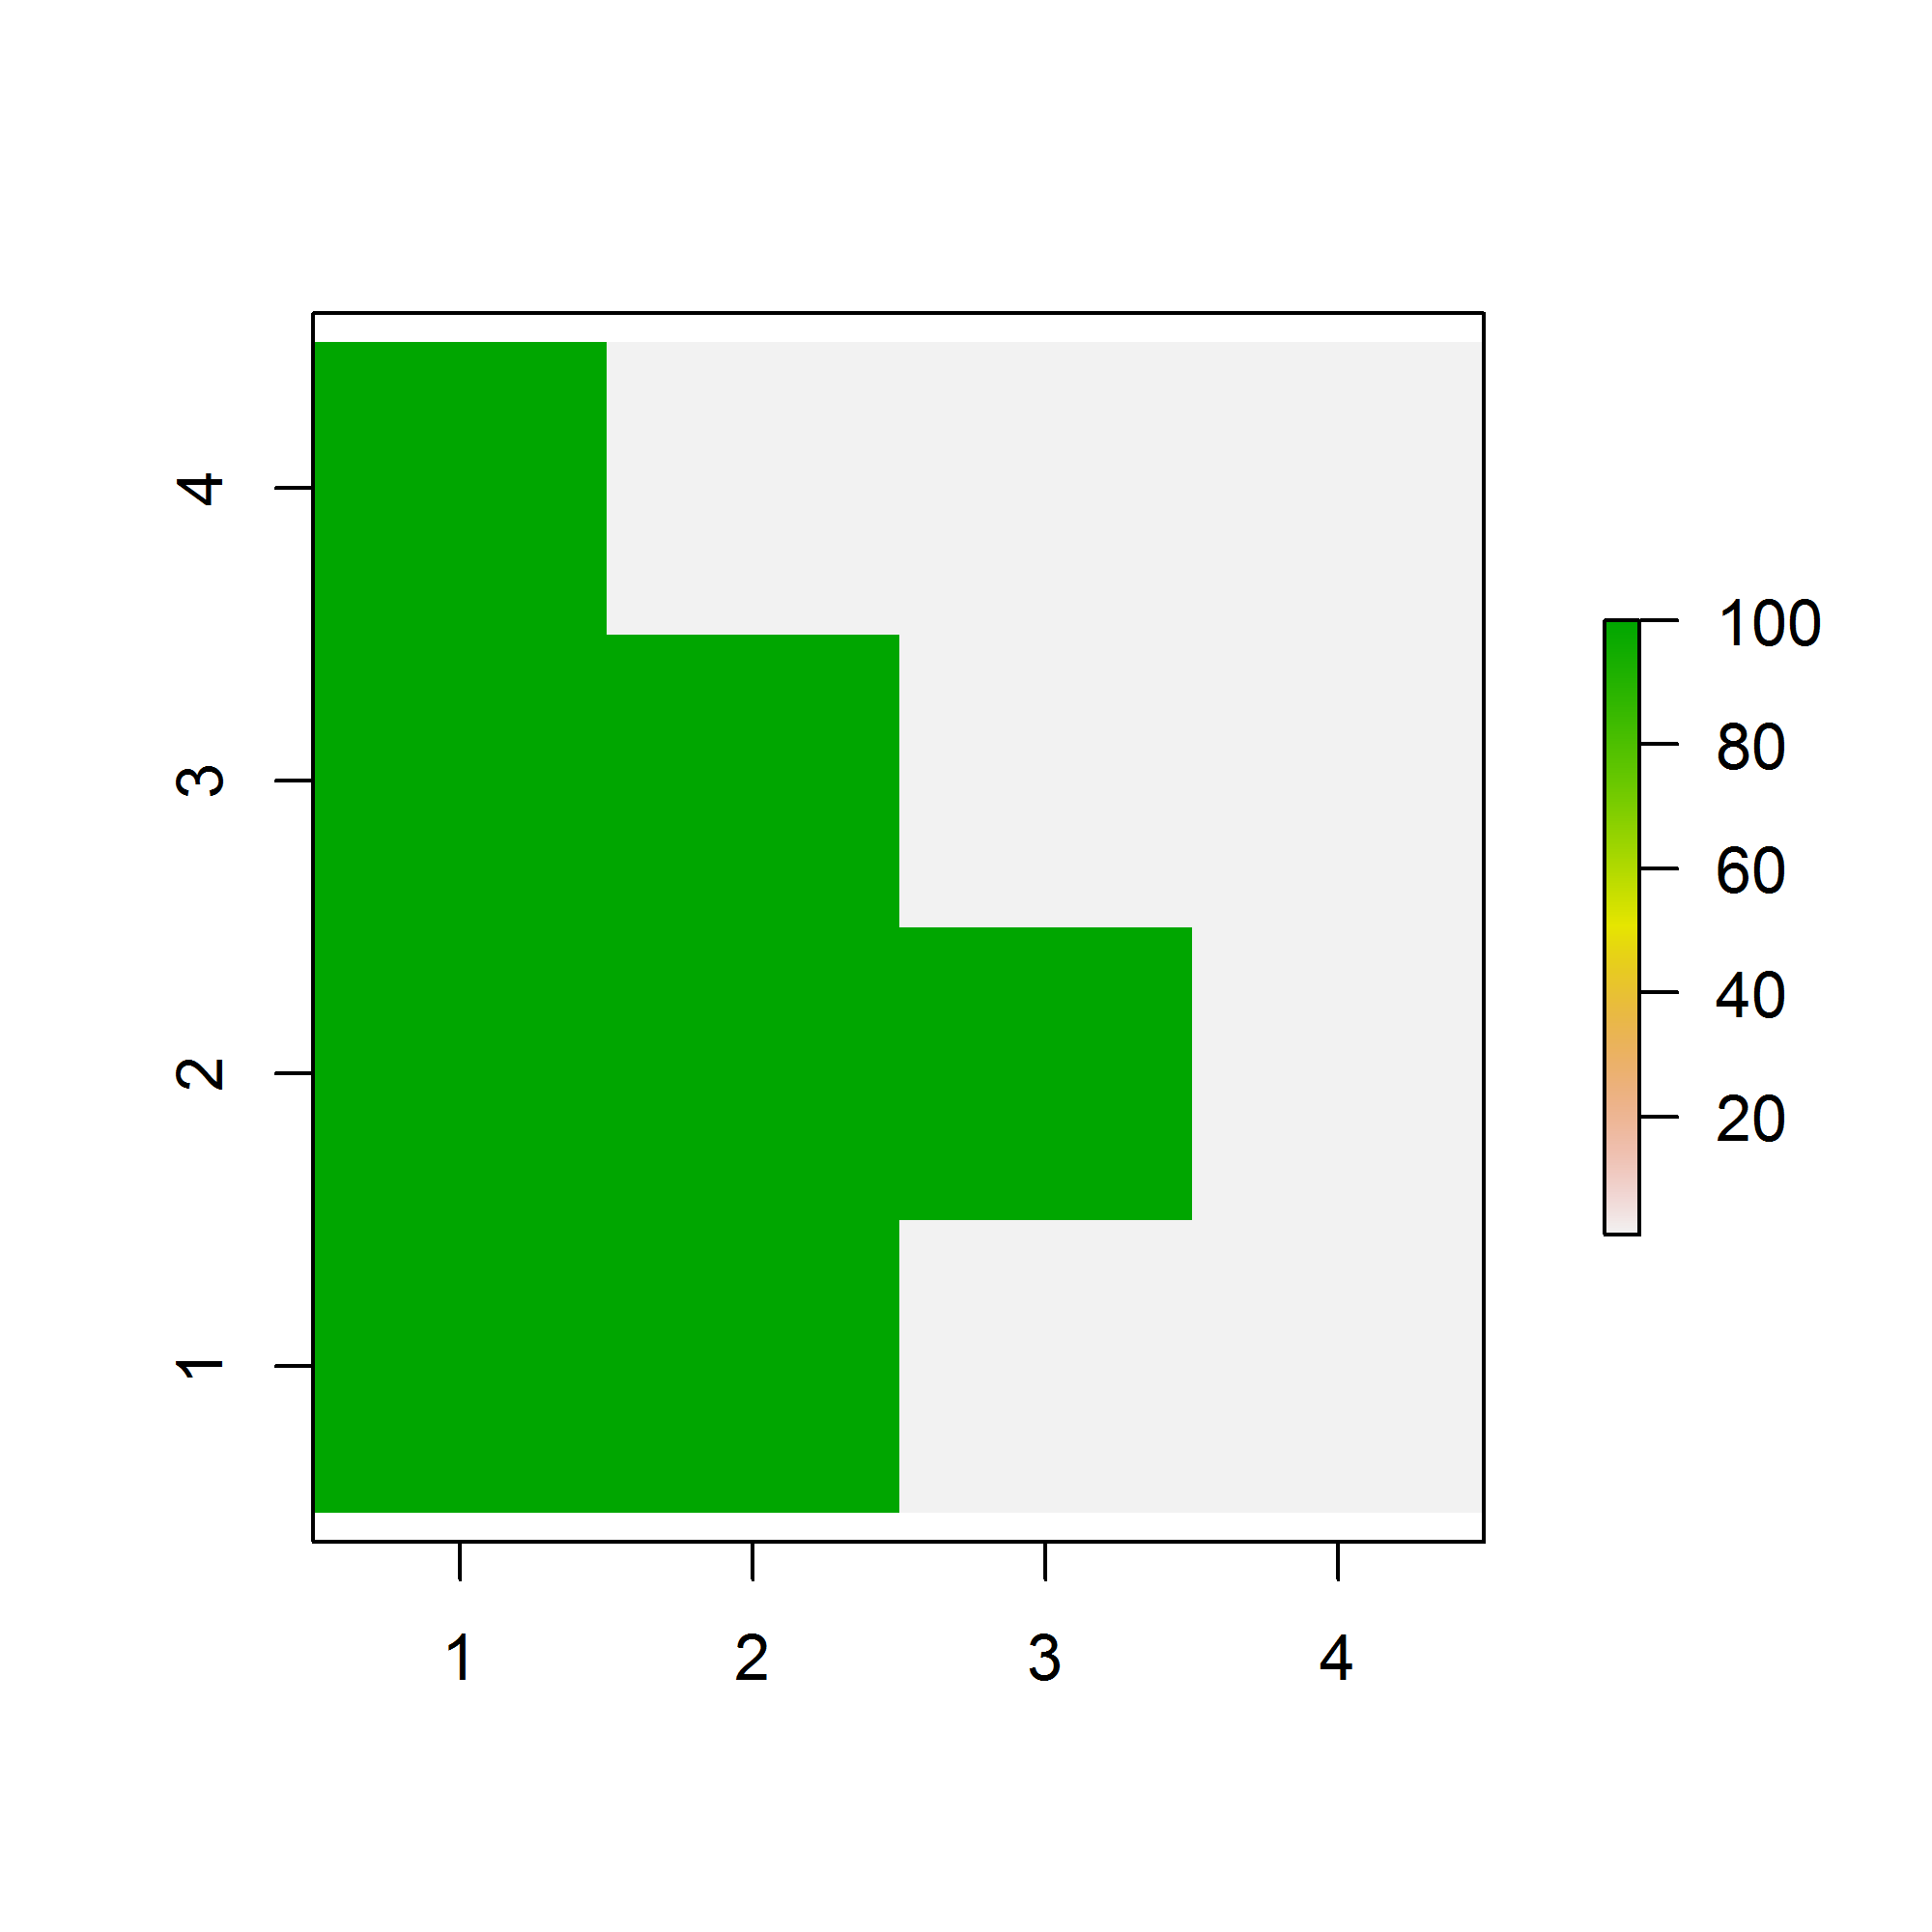
\includegraphics[height=3.25in,width=3.25in]{Ch12-EcolDist/figs/raster_2values}
\end{center}
\caption{A $4 \times 4$ raster depicting a binary cost surface, with cost = 1 (white) or 100 (shaded) to represent ease of movement across a pixel.}
\label{ecoldist.fig.raster}
\end{figure}

For this simple case we
 can easily compute the shortest cost-weighted distance between any
pixels ``by eye''.  For example, the shortest cost-weighted distance between
pixels 5 and 9 in this example is 50.5 units: $1*(100+1)/2 = 50.5$,
the shortest distance between pixels 4 and 8 is also 50.5, while the
shortest cost-distance between 4 and 12 is 51.5.  What is the shortest
distance between 7 and 16? Suppose an individual at pixel 7 can move
diagonal (which has distance $\sqrt{2}$) and pay $\sqrt{2}(100+1)/2$,
and then move once to the right to pay $1$ additional unit cost, for a
total of $72.4$. However, if the individual instead moved one unit to
the right, to pixel 11, and then diagonally, the total cost is
$51.914$ which is the minimum cost-weighted distance in getting from
pixel 7 to 16. These two ways of moving from 7 to 16 have the same
Euclidean distance, but different cost-weighted distances according to
our cost function.

The least-cost path distances can be
computed with just a couple {\bf R} commands, and these commands can
be inserted directly into the likelihood construction for an ordinary
spatial capture-recapture model. The {\bf R} package
\mbox{\tt gdistance} calculates least-cost path using  Dijkstra's algorithm
\citep{dijkstra:1959} (from the \mbox{\tt igraph} package
\citep{csardi:2010}).
%Using \mbox{\tt gdistance}, we
%define the incremental cost of moving from one pixel to another as the
%distance-weighted {\it average} of the 2 pixel costs. We demonstrate
%how to do this subsequently.
To compute the least-cost path, or the minimum cost-weighted distances
between every pixel and every other pixel, we make use of the helper
function \mbox{\tt transition}, which calculates the cost of moving
between neighboring pixels.  It operates on the inverse-scale
(``conductance''), and so the \mbox{\tt transitionFunction} argument
is given as $1/mean(x)$.  The function \mbox{\tt geoCorrection}
modifies this object depending on the projection of the coordinate
system (e.g., it corrects for curvature of the earth's surface if
longitude/latitude coordinates are used).  The result is fed into the
function \mbox{\tt costDistance} to compute the pair-wise distance
matrix. For that, we define the center points of each raster, here
these are just integers on $[1,4] \times [1,4]$.  The commands
altogether are as follows: {\small
\begin{verbatim}
> tr1<-transition(r,transitionFunction=function(x) 1/mean(x),directions=8)
> tr1CorrC<-geoCorrection(tr1,type="c",multpl=FALSE,scl=FALSE)
> pts<-cbind( sort(rep(1:4,4)),rep(4:1,4))
> costs1<-costDistance(tr1CorrC,pts)
> outD<-as.matrix(costs1)
\end{verbatim}
}
Now we can look at the result and see if it makes sense to us. Here we
produce the first 5 columns of this distance matrix to illustrate a
couple of examples of calculating the minimum cost-weighted distance
between points:
\begin{center}
{\small
\begin{verbatim}
> outD[1:5,1:5]
         1        2        3        4        5
1   0.0000 100.0000 200.0000 205.2426 100.0000
2 100.0000   0.0000 100.0000 200.0000 141.4214
3 200.0000 100.0000   0.0000 100.0000 126.1604
4 205.2426 200.0000 100.0000   0.0000 105.2426
5 100.0000 141.4214 126.1604 105.2426   0.0000
\end{verbatim}
}
\end{center}
An interesting case is that between point 1 and 4. Note that simply
taking the shortest Euclidean distance, weighted by cost, produces a
cost-weighted distance of $100 \times 1$ to move from pixel 1 to pixel
2, and similarly from 2 to 3 and 3 to 4, producing a total
cost-weighted distance of $300$. However, the actual {\it least-cost
  path} has cost-weighted distance $205.2426$. See if you can figure
out the shortest path by inspection.

The key point here is that, once we can compute this distance matrix,
we can use it as the distance matrix in computing the encounter
probability between acctivity centers and traps, and we can use our
existing MLE technology (Chapt. \ref{chapt.mle}) to fit models that
are based on ecological distance.



\section{Simulating SCR Data using Ecological Distance}
\label{ecoldist.sec.simulating}

\citet{royle_etal:2012ecol} simulated capture-recapture data
%in the presence of
such that landscape connectivity was governed by %using
a cost function having a
single covariate, and they considered two hypothetical covariate
landscapes
(Fig. \ref{ecoldist.fig.raster100}).
%typical of how
%cost-weighted distance models might be used in real capture-recapture
%problems.
The landscape here is a $20 \times 20$ pixel raster, with
extent = $[0.5, 4.5] \times [0.5, 4.5]$.
For example, think of each pixel as
representing, say, a $1 \times 1$ km grid cell with something like
``percent developed'' or ``trail/road density'' representing the
covariate. For sampling by capture-recapture, imagine
that 16 camera traps are established at the integer coordinates
$(1,1), (1,2), \ldots, (4,4)$.
The two covariates were constructed as follows (see \mbox{\tt
  ?make.EDcovariates} for the {\bf R} commands):
First is an increasing trend from
the NW to the SE (``systematic covariate''), where $C({\bf x})$ is defined as
$C({\bf x}) = row({\bf x}) + col({\bf x})$ and $row({\bf x})$ and $col({\bf x})$ are just the row and
column, respectively, of the raster.  This might mimic something
related to distance from an urban area or a gradient in habitat
quality due to land use, or environmental conditions such as
temperature or precipitation gradients.  In the second case we make up
a covariate by generating a field of spatially correlated noise to
emulate a typical patchy habitat covariate (``patchy covariate'') such as
tree or understory density.

For both covariates we use a
cost function in which transitions from pixel ${\bf x}$ to ${\bf x}'$
is given by:
\[
 \log(\mbox{cost}({\bf x},{\bf x}'))=  \alpha_2 \left( \frac{C({\bf
       x}) + C({\bf x}')}{2} \right)
\]
where $\alpha_2 = 1$ for simulating the observed data.
 Remember that with $\alpha_2=0$ the
model reduces to one in which the cost of moving across each pixel is
constant, and therefore Euclidean distance is operative.
In the left panel of
Fig. \ref{ecoldist.fig.raster100}, a sample realization of
$N=100$ activity centers is shown. While encounter probability is
assumed to be related to landscape connectivity according to the
single-variable cost function, individual activity centers are
assumed to be uniformly distributed, although we can modify this
assumption (See Sec.~\ref{chapt.ecoldist.sec.ssed} below).


\begin{figure}[h]
\begin{tabular}{ll}
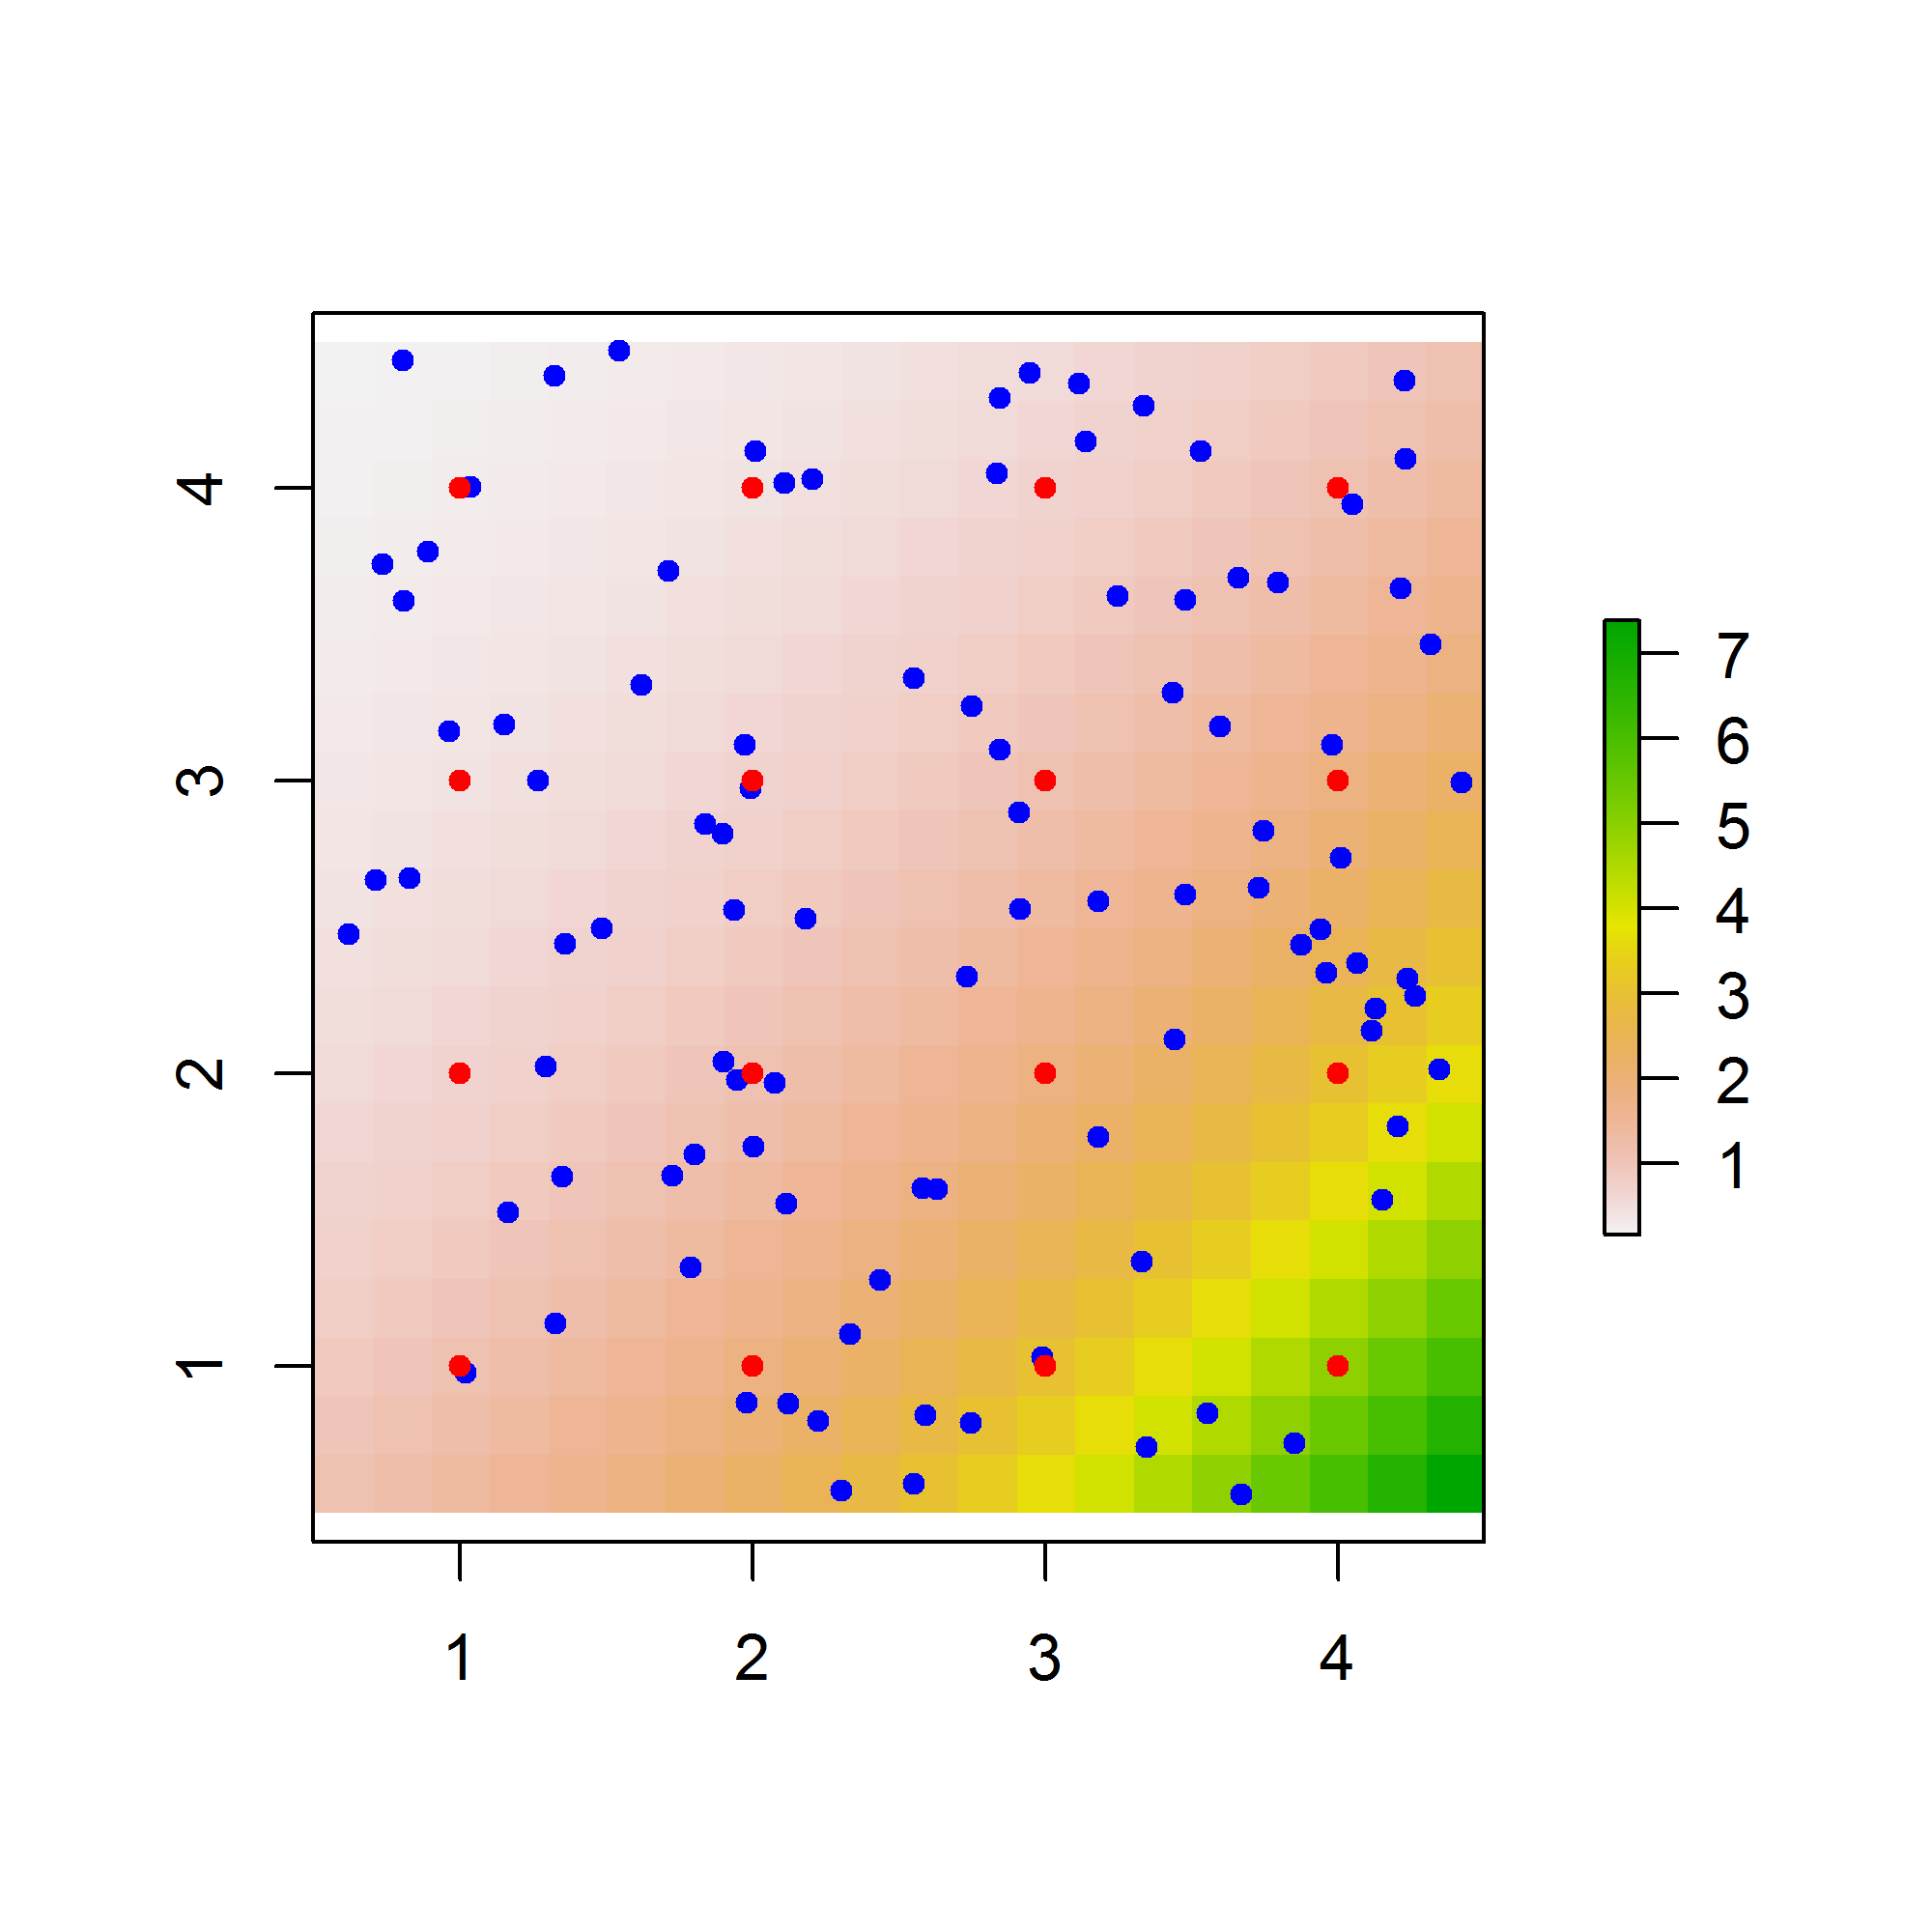
\includegraphics[height=2.5in,width=2.5in]{Ch12-EcolDist/figs/raster_withN100}
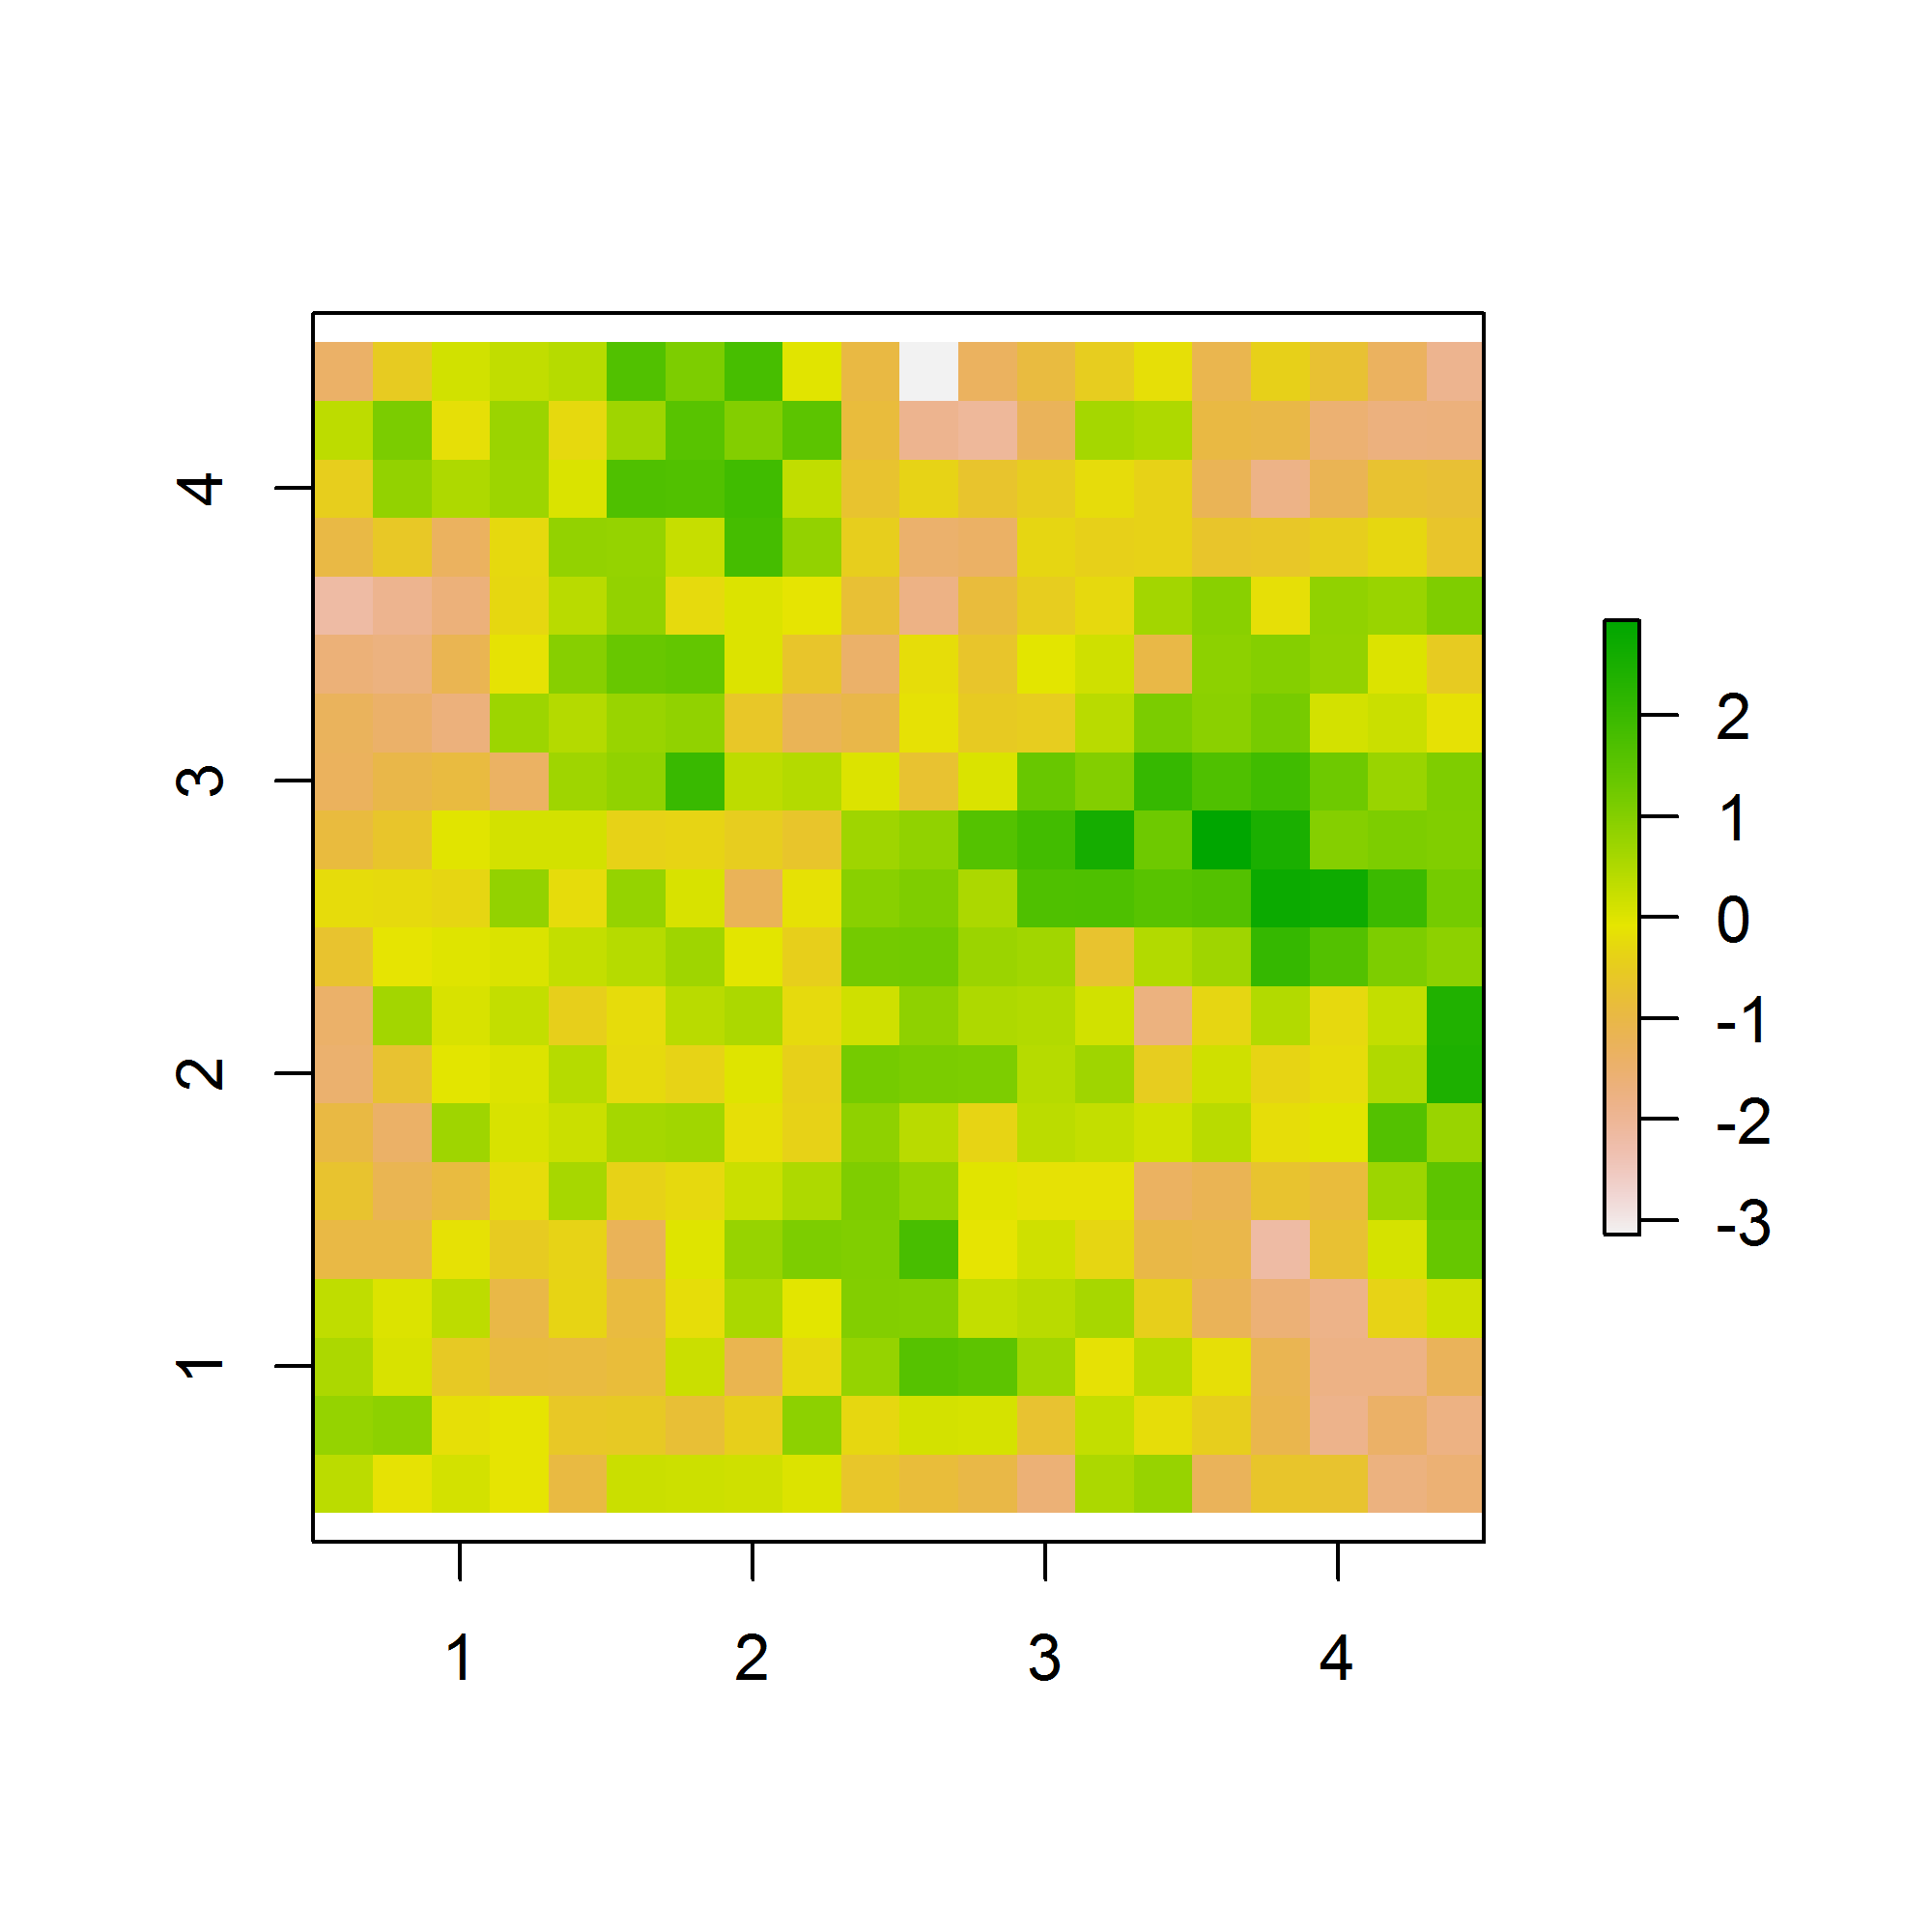
\includegraphics[height=2.5in,width=2.5in]{Ch12-EcolDist/figs/raster_krige} &
\end{tabular}
\caption{Two covariates (defined on a $20 \times 20$ grid) used in simulations.
 Left panel shows a covariate with systematic structure meant
to mimic distance from some feature, and the right panel shows a ``patchy'' covariate.
A hypothetical realization of $N=100$ activity centers (blue dots) is superimposed
  on the left figure, along with 16 trap locations. }
\label{ecoldist.fig.raster100}
\end{figure}


When distance is defined by the cost-weighted distance metric given
by Eq. \ref{eq.lcp} then individual space-usage varies
spatially in response to the landscape covariate(s) used in the
distance metric.  As a consequence, home range contours are no longer
circular, as in SCR models based on Euclidean distance.
For example, using one of the covariates we use in
our simulation study below (Fig. \ref{ecoldist.fig.raster100}, right
panel) with a Gaussian
%pdf detection function
encounter model but having distance
metric defined by Eq. \ref{eq.lcp}, produces home ranges such
as those shown in Fig. \ref{fig.homeranges}.


\begin{figure}
\begin{center}
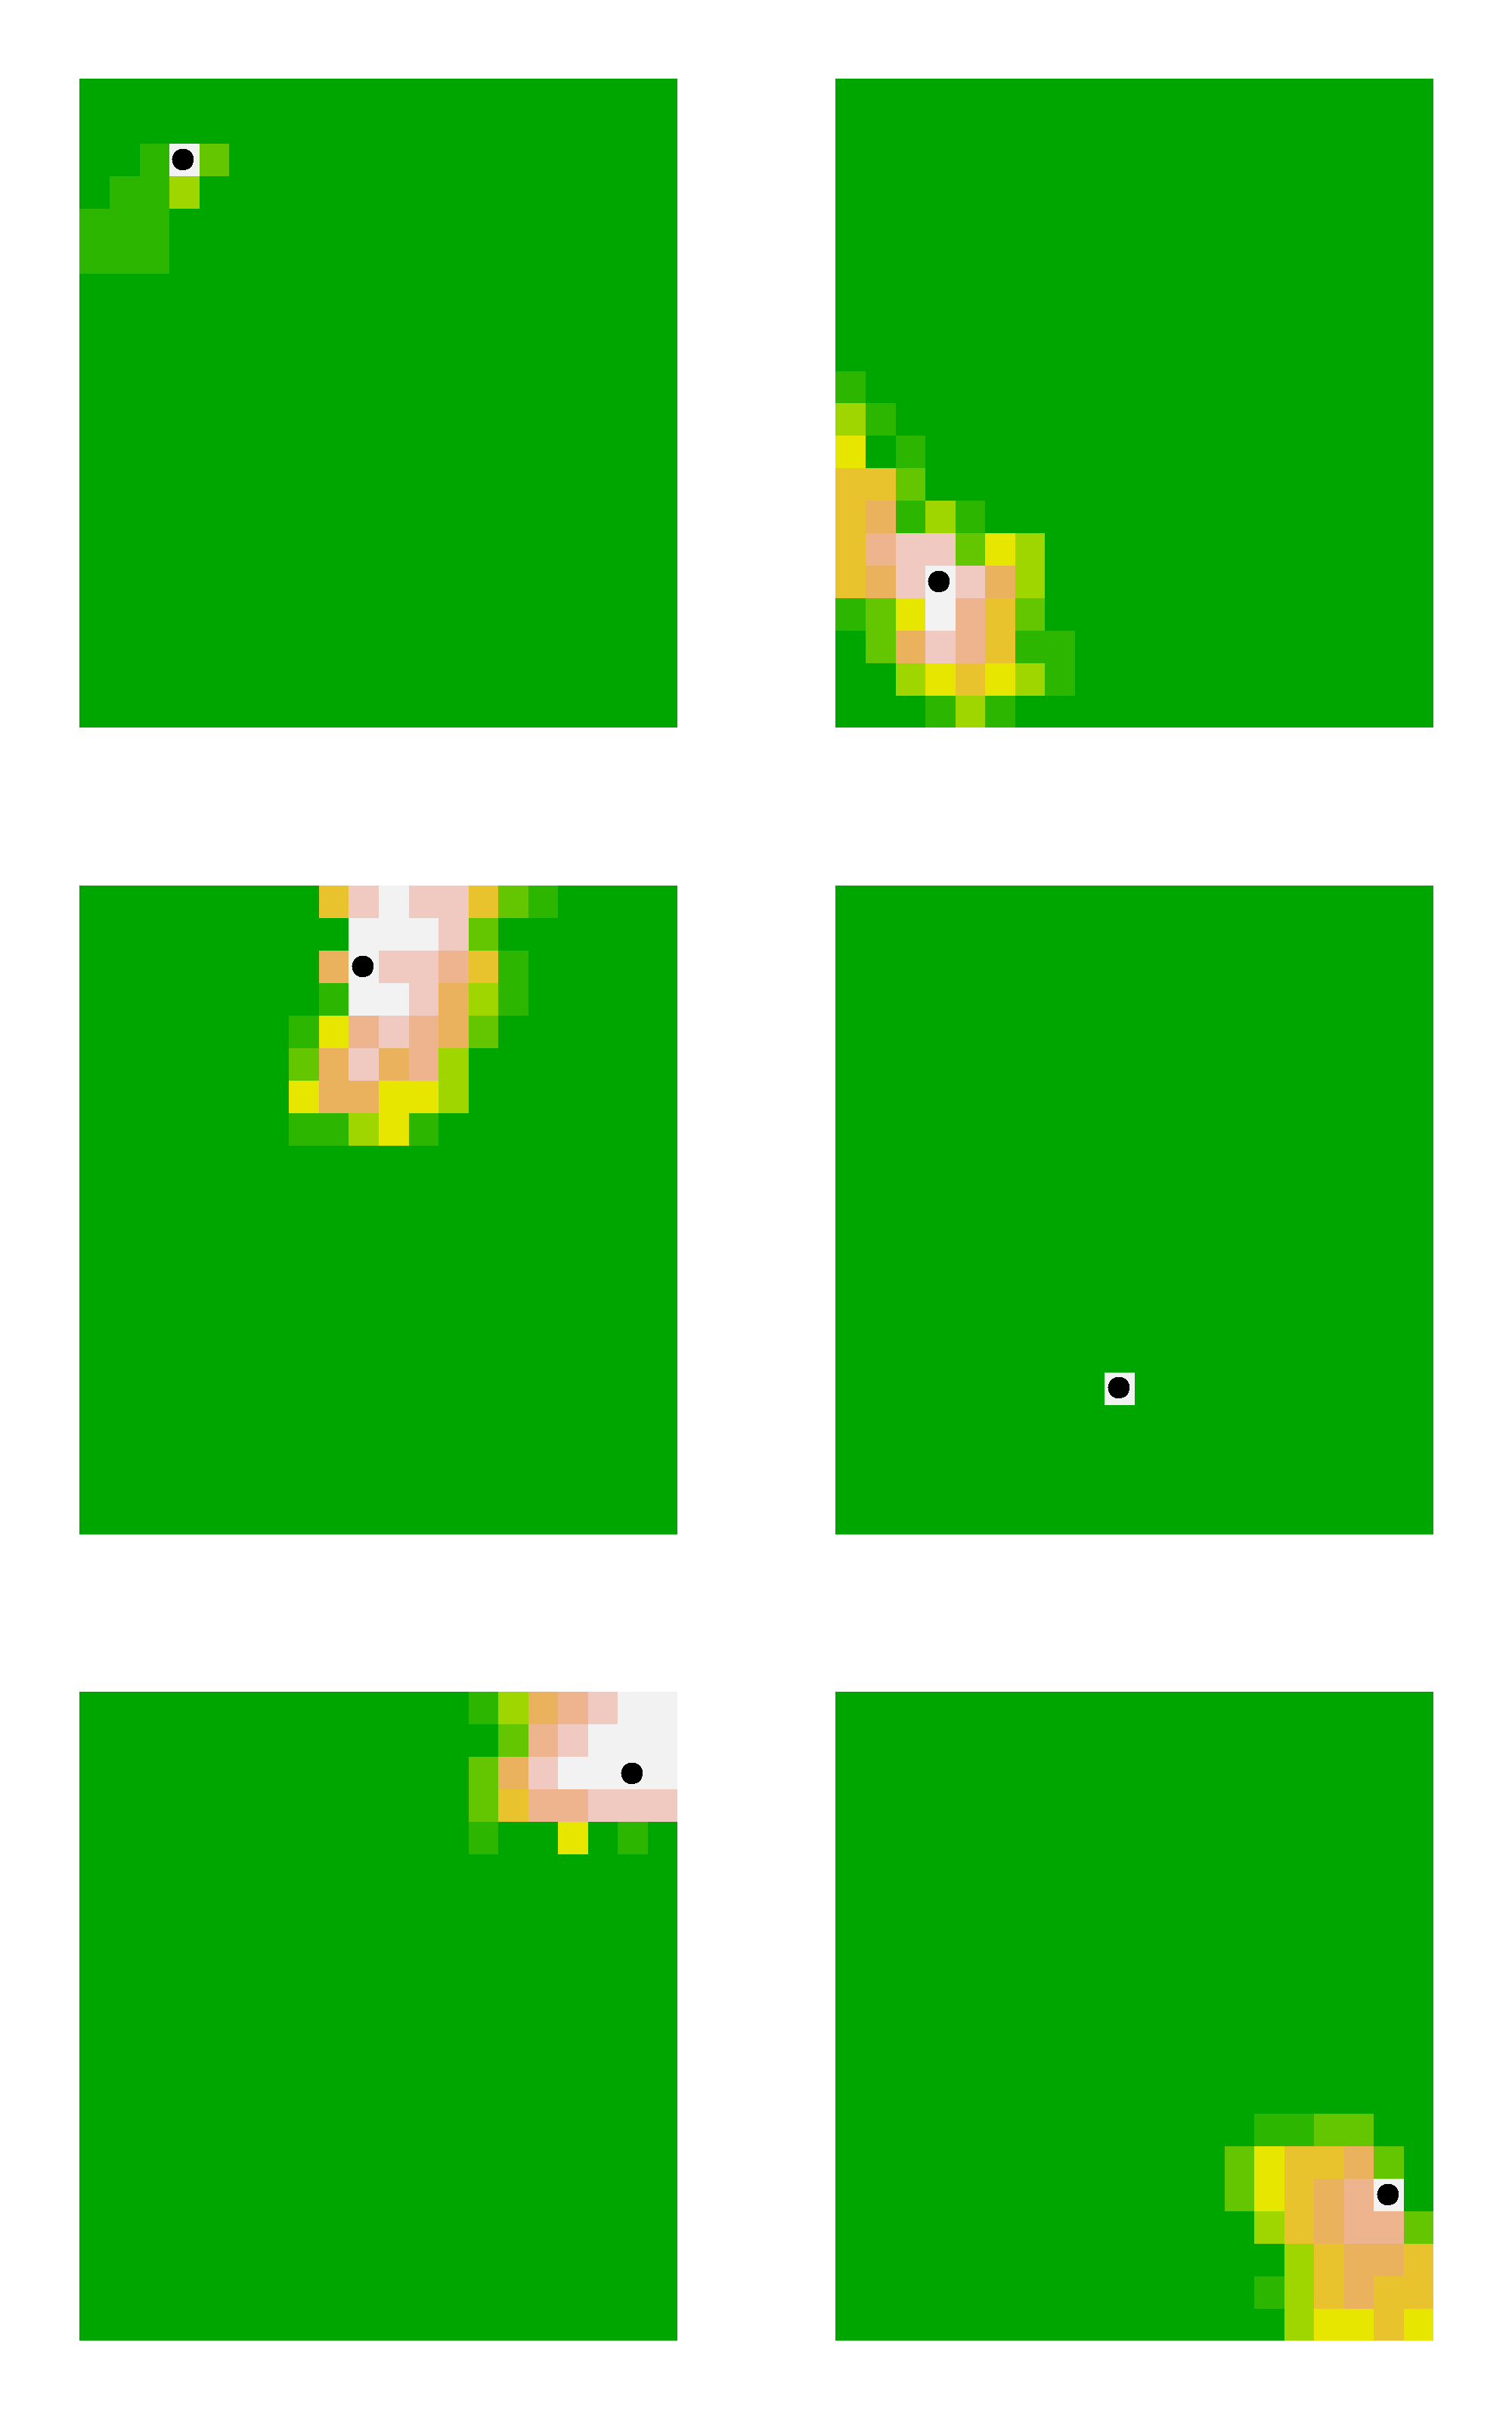
\includegraphics[height=6in,width=3.75in]{Ch12-EcolDist/figs/home_ranges}
\end{center}
\caption{
Typical home ranges for 6 individuals based on the cost surface shown in the right panel of
  Fig. \ref{ecoldist.fig.raster100} with $\alpha_{2}=1$. The black dot indicates the home
  range center and the pixels around each home range center are shaded
according to the probability of encounter, if a trap were located in
that pixel.
}
\label{fig.homeranges}
\end{figure}

To simulate data,
 we have to load the \mbox{\tt
scrbook} package and call the function \mbox{\tt make.EDcovariates} to generate
our raster covariates (see the help file for how that is done). We
process the covariate into a least-cost path distance
matrix, and then simulate observed encounter data using standard methods
which we have used many times previously in this book. The complete set
of {\bf R} commands is:
{\small
\begin{verbatim}
### Grab a covariate
library(scrbook)
set.seed(2013)
out<-make.EDcovariates()
covariate<-out$covariate.patchy

### prescribe some settings
N<-200
alpha0<- -2
sigma<- .5
alpha1<- 1/(2*sigma*sigma)
alpha2<-1
K<- 5
S<-cbind(runif(N,.5,4.5),runif(N,.5,4.5))

# make up some trap locations
xg<-seq(1,4,1); yg<-4:1
traplocs<-cbind( sort(rep(xg,4)),rep(yg,4))
points(traplocs,pch=20,col="red")
ntraps<-nrow(traplocs)

### make a raster and fill it up with the "cost"
r<-raster(nrows=20,ncols=20)
projection(r)<- "+proj=utm +zone=12 +datum=WGS84"
extent(r)<-c(.5,4.5,.5,4.5)
cost<- exp(alpha2*covariate)

### compute least-cost path distance
tr1<-transition(cost,transitionFunction=function(x) 1/mean(x),directions=8)
tr1CorrC<-geoCorrection(tr1,type="c",multpl=FALSE,scl=FALSE)
D<-costDistance(tr1CorrC,S,traplocs)
probcap<-plogis(alpha0)*exp(-alpha1*D*D)

# now generate the encounters of every individual in every trap
# discard uncaptured individuals
Y<-matrix(NA,nrow=N,ncol=ntraps)
for(i in 1:nrow(Y)){
 Y[i,]<-rbinom(ntraps,K,probcap[i,])
}
Y<-Y[apply(Y,1,sum)>0,]
\end{verbatim}
}


\section{Likelihood Analysis of Ecological Distance Models}
\label{ecoldist.sec.mle}

Throughout much of this book we rely on Bayesian analysis by MCMC
mostly using {\bf BUGS}, but sometimes (as in Chapt. \ref{chapt.mcmc})
developing our own implementations. However, occasionally we prefer to
use likelihood estimation, such as when we can compare a set of models
directly by likelihood either to do a direct hypothesis test of a
parameter, or to tabulate a bunch of AIC values. For the class of
models that use least-cost path, we also prefer likelihood methods not
because they have any conceptual or methodological benefit, but simply
because they are more computationally efficient to implement
\citep{royle_etal:2012ecol}.

There are no technical considerations in adapting our formulation of
maximum likelihood estimation \citep{borchers_efford:2008} from
Chapt. \ref{chapt.mle} for the class of models based on least-cost
path (see the appendix in \citet{royle_etal:2012ecol} for complete details).
Likelihood analysis is really just a straightforward adaptation in which we
replace the Euclidean distance with least-cost path.  Consider the
Bernoulli model in which the individual- and trap-specific
observations have a binomial distribution conditional on the latent
variable ${\bf s}_{i}$:
\begin{equation}
  y_{ij}| {\bf s}_{i} \sim \mbox{Binomial}(K, p_{\bm \alpha}(d_{lcp}({\bf x}_{j},{\bf s}_{i};\alpha_{2}); \alpha_{0}, \alpha_{1})
\label{ecoldist.eq.cond-on-s}
\end{equation}
where we have indicated the dependence of $p$ on the parameters
${\bm \alpha} =(\alpha_{0},\alpha_{1},\alpha_{2})$, and also $d_{lcp}$ which
itself depends on $\alpha_{2}$, and the latent variable ${\bf s}_i$.
We note that the only difference between likelihood analysis of this
model and the standard Bernoulli model, is the use of $d_{lcp}$ here.
For the random effect we have ${\bf s}_{i} \sim  \mbox{Uniform}({\cal
  S})$, we can easily compute the integrated (marginal) likelihood of
an encounter history.
The likelihood is given in the {\tt scrbook} package as the function
\mbox{\tt intlik3ed}. The help file
provides an example of its usage and for simulating data.
To use this function the cost covariate $C({\bf x})$ has to be of class
\mbox{\tt RasterLayer} which requires packages \mbox{\tt sp} and
\mbox{\tt raster} to manipulate.


\subsection{Example of SCR with least-cost path}

Now we use the {\bf R} function \mbox{\tt nlm} along with
our \mbox{\tt intlik3ed} function to  obtain the MLEs of the
model parameters for the data simulated
in Sec. \ref{ecoldist.sec.simulating}.
 We'll do that for both the standard Euclidean distance
and then for the ecological distance based on the ``patchy''
covariate using the following commands:
{\small
 \begin{verbatim}
> frog1<-nlm(intlik3ed,c(alpha0,alpha1,3)),hessian=TRUE,y=Y,K=K,X=traplocs,
               distmet="euclid",covariate=covariate,alpha2=1)

> frog2<-nlm(intlik3ed,c(alpha0,alpha1,3,-.3),hessian=TRUE,y=Y,K=K,X=traplocs,
               distmet="ecol",covariate=covariate,alpha2=NA)
\end{verbatim}
}
The summary output for the two model fits is shown in Table \ref{ecoldist.tab.results1}.
The model based on least-cost path (the data generating model) appears
to be much preferred in terms of negative log-likelihood.
The output parameter order is $(\alpha_{0}, \alpha_{1}, \log(n_{0}), \text{and}
\log(\alpha_{2}))$ (remember, we want to keep $\alpha_{2}$
positive, so it's logarithm is estimated).
The data generating parameter values were
$\alpha_{0} = - 2$,
$\alpha_{1} = 2$ and $\log(\alpha_{2}) = 0$.
The simulated sampling produced a sample of 96 individuals and so the
number of individuals not captured is
$n_{0} = 104$, and $\log(n_{0}) = 4.64$. We see that the
 MLEs of the least-cost path model are pretty close whereas they are
 not so close under the misspecified model based on Euclidean distance.



\begin{table}
\caption{
Summary output of fitting models based on Euclidean and least-cost
path distance to simulated data using the
 \mbox{\tt intlik3ed} function (see \mbox{\tt ?intlik3ed}). Data were
 simulated based on the least-cost path model using the ``patchy''
 covariate shown in Fig. \ref{ecoldist.fig.raster100}.
}
\begin{tabular}{cccccc} \hline \hline
Distance metric &  -loglik &     $\alpha_0$  & $\alpha_1$  &\mbox{log}($n_{0}$) &  $\alpha_2$ \\ \hline
True value      &          &         -2      &    2       &   4.644 & 1 \\
Euclidean   &133.495&  -1.885 &    1.247 &    3.549 &      -- \\
Least-cost path (truth) & 70.119& -1.780 &  2.471    &    4.459 &
0.046  \\ \hline
\end{tabular}
\label{ecoldist.tab.results1}
\end{table}






\section{Bayesian Analysis}

While implementation of these ecological distance SCR models is
reasonably straightforward, the model cannot be fitted
in the  {\bf BUGS} engines because least-cost path distance cannot be computed.
It would be possible to fit the models
in {\bf BUGS} if the parameter $\alpha_{2}$ was fixed. In that case,
one could compute the distance matrix ahead of time and reference the
required elements for a given ${\bf s}$.
Alternatively, it would be possible to write a custom MCMC routine
using the methods we present in Chapt. \ref{chapt.mcmc}, although we
have not yet developed our own MCMC implementation of SCR models with
ecological distance metrics.


\section{Simulation Evaluation of the MLE}

\citet{royle_etal:2012ecol}
carried-out a limited simulation study to evaluate the
general statistical performance of the density estimator under
this new model, the effect of mis-specifying the model with a
normal Euclidean distance metric, and evaluate the general bias and
precision properties of the MLE using the systematic and patchy
landscapes shown in
Fig. \ref{ecoldist.fig.raster100}.

Their results showed extreme
bias in estimates of $N$ when the misspecified Euclidean distance is
used, and only negligible small-sample
 bias of 3-5\% in the MLE of $N$ using the
least-cost distance which becomes negligible as the expected seample
size increases (either due to increasing $K$, or larger population sizes).
The performance of estimating the other parameters, including the
cost parameter $\alpha_{2}$ mirrors
the results for estimating $N$.
We reproduce a subset of the results from \citet{royle_etal:2012ecol}
%here,
in Table \ref{ecoldist.tab.simresults}.

\begin{table}[htp]
\label{tab.results1}
{\small
\caption{
Simulation results for estimating population size $N$ for a prescribed state-space with
$N=100$ or $N=200$ and various levels of replication ($K$)
using the ``patchy'' landscape shown in Fig.
 \ref{ecoldist.fig.raster100}.
For each simulated
data set, the SCR model was fitted by maximum likelihood with
standard Euclidean distance (``euclid''), or least-cost path
(``lcp''), which was the true data-generating model.
The summary statistics of the
sampling distribution reported are the mean, standard deviation
(``SD'') and quantiles (0.025, 0.50, 0.975).
}
\begin{tabular}{l|rrrrr}
  \hline
         & \multicolumn{5}{c}{N=100  }  \\ \hline
         &   mean &  SD  & 0.025 & 0.50  & 0.975   \\ \hline
$K=3$      &        &      &       &       &         \\
euclid   &  78.68 & 18.12& 49.40 & 76.34 & 125.47  \\
lcp      & 110.96 & 28.65& 69.55 &106.98 & 181.84  \\
$K=5$     &        &      &       &       &         \\
euclid   &  77.85 & 11.55& 59.17 & 77.44 & 101.14  \\
lcp      & 104.44 & 15.79& 78.38 &101.47 & 139.55  \\
$K=10$     &        &      &       &       &         \\
euclid   &  78.01 & 5.26 & 68.00 & 77.96 & 87.81   \\
lcp      & 100.42 & 7.56 & 86.72 &100.34 & 115.47  \\ \hline
        & \multicolumn{5}{c}{N=200   }  \\ \hline
$K=3$      &        &      &       &       &         \\
euclid  154.34& 33.74& 107.00& 146.34& 221.43\\
lcp     208.77& 49.29& 141.68& 197.89& 325.77\\
$K=5$           &      &       &       &        \\
euclid   153.39& 15.57& 129.31& 149.54& 185.38\\
lcp      200.91& 20.78& 164.42& 200.47& 246.46\\
$K=10$           &      &       &       &       \\
euclid   156.27&  8.51& 142.17& 156.05& 174.55\\
lcp      198.45& 11.44& 180.06& 198.04& 219.52\\ \hline
\end{tabular}
}
\label{ecoldist.tab.simresults}
\end{table}














\begin{comment}
For population sizes of 100 and 200, individuals with activity
centers randomly distributed on the $20 \times 20$ landscape, they
subjected individuals
to encounter by 16 traps arranged in a $4\times 4$ grid
using a Gaussian
encounter model with least-cost path distance metric:
\[
\log(p_{ij})= \alpha_{0} + \alpha_{1} d_{lcp}({\bf x}_{j},{\bf
  s}_{i}; \alpha_{2})^{2}
\]
where  $\alpha_{0} = -2$ and $\alpha_{1} = 2$, the latter value
corresponding to $\sigma = 0.5$ of a stationary bivariate normal home
range model.  Different numbers of replicate samples were considered,
$K=3,5,10$
(e.g., nights in a camera trapping study), in order
to produce varying sample
sizes.
For each of the ``systematic'' and ``patchy'' landscapes defined
previously, 200 data sets were simulated and, for each of those, two
different models were fitted: the misspecified Euclidean distance
model; and (ii) the true data-generating model but estimating the
relative cost parameter by maximum likelihood.
\end{comment}


%%%%%%%%%%%% \subsection{Simulation Results}
\begin{comment}
For both landscapes and all simulation conditions (levels of $K$ and
$N$) the average sample sizes of individuals captured are given in
Tab. \ref{tab.samplesize}.
\begin{table}[h]
\centering
\caption{
Expected sample sizes of captured individuals under each configuration of
$N$ (population size for the prescribed state-space) and $K$ (number of replicate samples).
}
\begin{tabular}{l|rrrr}
 & \multicolumn{2}{c}{Systematic} & \multicolumn{2}{c}{Patchy}  \\
    & N=100 &  N=200  &   N=100 &  N=200  \\ \hline
K=3 &  38.69 &   78.17  &   37.30 &   74.93  \\
K=5 &  51.10 &  103.18  &   51.89 &  103.71 \\
K=10&  65.81 &  132.39  &   69.44 &  138.76 \\
\end{tabular}
\label{tab.samplesize}
\end{table}
The simulation results for estimating $N$
for the prescribed state-space are presented in Tab.
\ref{tab.results1}.  For the ``patchy'' landscape we see extreme
bias in estimates of $N$ when the Euclidean distance is used. There is
moderate small sample bias of 3-5\% in the MLE of $N$ using the
least-cost distance which becomes negligible as $K$ increases. For
$N=200$ the bias is on the order of 2\% for the lowest sample size
case ($K=3$) but negligible otherwise.  Interestingly, for the
landscape exhibiting systematic structure, there is a persistent bias
in the MLE of $N$ of 1-3\% even for the highest level of $K$.
As noted by \citet{royle_etal:2012ecol},
this is due to the fact that
the state-space is small relative to the extent of the trapping grid and
sensitivity to a state-space that is too small is expected because the
support of the integrand is truncated. In the particular case of the
systematic landscape, we find that, in the NW corner of the raster
where cost of movement is low, individuals use large areas of space,
and the fitted model is under-stating the apparent
heterogeneity in encounter probability for the prescribed raster.  \citet{royle_etal:2012ecol}
found that the issue is resolved when the traps are moved away from
the boundary (results shown in Tab. \ref{tab.results3}).

The performance of estimating the cost parameter $\alpha_{2}$ mirrors
the results for estimating $N$ for the prescribed state space. In the
patchy landscape where we don't expect a systematic gradient in space
usage around the edge of the state-space, we see
(Table \ref{tab.results2}) that $\alpha_{2}$ is estimated with
diminishing bias as the sample size increases, but with persistent
bias due to truncation of the likelihood under the systematic
landscape which, as with the MLE of $N$, is resolved by moving the
traps away from the edge of the raster. Equivalently, in practice,
this could be resolved by expanding the raster away from the trap
locations so that all regions used by animals exposed to capture are
included in the state-space.
















\begin{table}[htp]
\label{tab.results1}
{\small
\caption{Simulation results for estimating population size $N$ for a prescribed state-space with
$N=100$ or $N=200$ and various levels of replication ($K$) chosen to affect the observed sample
size of individuals (Tab. \ref{tab.samplesize}). For each simulated
data set, the SCR model was fitted by maximum likelihood with
standard Euclidean distance (``euclid''), or least-cost path
(``lcp''), which was the true data-generating model.
The summary statistics of the
sampling distribution reported are the mean, standard deviation
(``SD'') and quantiles (0.025, 0.50, 0.975).
}
{\bf Systematic trend raster:} \\
\begin{tabular}{l|rrrrr|rrrrr}
         & \multicolumn{5}{c}{N=100   } & \multicolumn{5}{c}{N=200  }  \\
         &   mean &  SD  & 0.025 & 0.50 & 0.975  & mean  & SD   & 0.025 & 0.50  & 0.975 \\ \hline
K=3      &        &      &       &      &        &       &      &       &       &       \\
euclid   &   63.65& 12.62& 44.77 & 61.17&  90.98 & 126.68& 17.05&  98.93& 124.49& 168.26 \\
lcp      &  101.93& 21.68& 67.95 &101.56& 156.21 & 201.58& 28.14& 154.96& 200.15& 263.20\\
K=5      &        &      &       &      &        &       &      &       &       &        \\
euclid   &  64.60 & 7.11 & 51.52 & 63.86&  77.33 & 130.02& 10.25& 113.48& 128.96& 151.32\\
lcp      &  98.94 &12.97 & 74.68 & 99.00& 123.88 & 198.80& 19.60& 166.87& 197.97& 239.46\\
K=10     &        &      &       &      &        &       &      &       &       &       \\
euclid   &  69.24 & 4.83 & 59.37 & 69.47&  79.18 & 139.83&  7.62& 125.65& 139.65& 154.82\\
lcp      &  97.53 & 8.18 & 82.02 & 97.62& 113.16 & 195.19& 13.28& 171.63& 194.58& 217.96\\ \hline
\end{tabular}
\\
{\bf Patchy ``random'' raster: } \\
\begin{tabular}{l|rrrrrrrrrr}
         & \multicolumn{5}{c}{N=100  } & \multicolumn{5}{c}{N=200   }  \\
         &   mean &  SD  & 0.025 & 0.50  & 0.975  & mean  & SD   & 0.025 & 0.50  & 0.975 \\ \hline
K=3      &        &      &       &       &        &       &      &       &       &       \\
euclid   &  78.68 & 18.12& 49.40 & 76.34 & 125.47 & 154.34& 33.74& 107.00& 146.34& 221.43\\
lcp      & 110.96 & 28.65& 69.55 &106.98 & 181.84 & 208.77& 49.29& 141.68& 197.89& 325.77\\
K=5      &        &      &       &       &        &       &      &       &       &        \\
euclid   &  77.85 & 11.55& 59.17 & 77.44 & 101.14 & 153.39& 15.57& 129.31& 149.54& 185.38\\
lcp      & 104.44 & 15.79& 78.38 &101.47 & 139.55 & 200.91& 20.78& 164.42& 200.47& 246.46\\
K=10     &        &      &       &       &        &       &      &       &       &       \\
euclid   &  78.01 & 5.26 & 68.00 & 77.96 & 87.81  & 156.27&  8.51& 142.17& 156.05& 174.55\\
lcp      & 100.42 & 7.56 & 86.72 &100.34 & 115.47 & 198.45& 11.44& 180.06& 198.04& 219.52\\ \hline
\end{tabular}
}
\end{table}

















\begin{table}[htp]
\centering
\caption{
Mean of sampling distribution of the cost function parameter
$\alpha_{2}$ for the different simulation
conditions.
}
\begin{tabular}{l|rrrr}
 & \multicolumn{2}{c}{Patchy} & \multicolumn{2}{c}{Systematic} \\
    & N=100 &  N=200  &   N=100 &  N=200  \\ \hline
$K=3$  &   1.05&    1.03 &     1.17 & 1.14 \\
$K=5$  &   1.02&    1.01 &     1.12 &1.12 \\
$K=10$ &   1.01&    1.00 &     1.10 &1.08 \\
\end{tabular}
\label{tab.results2}
\end{table}




\begin{table}[htp]
{\tiny
\caption{Simulation results for estimating population size $N$ for a prescribed state-space with
$N=100$ or $N=200$ and various levels of replication ($K$) chosen to affect the observed sample
size of individuals. These results correspond to those of the
systematic landscape in Table XXXXXXX  except with the traps
moved 0.5 units in from the boundary of the landscape.
Each grouping of 2 rows (for a given value of $K$) summarizes the
performance of $\hat{N}$ under models based on
Euclidean distance  (``euclid'') and
a model based on least-cost path, which was the true data-generating model.
The summary statistics of the
sampling distribution reported are the mean, standard deviation
(``SD'') and quantiles (0.025, 0.50, 0.975).
}
\begin{tabular}{l|rrrrr|rrrrr}
         & \multicolumn{5}{c}{N=100   } & \multicolumn{5}{c}{N=200  }  \\
         &   mean &  SD  & 0.025 & 0.50 & 0.975  & mean  & SD   & 0.025 & 0.50  & 0.975 \\ \hline
K=3      &        &      &       &      &        &       &      &       &       &       \\
euclid   &   84.48& 20.42& 51.16 & 81.51& 140.62 &163.70 &24.55 &126.64 &157.67 &223.63 \\
lcp      &  105.90& 26.19& 65.95 &103.40& 182.30 &201.34 &29.54 &161.88 &192.36 &268.98\\
K=5      &        &      &       &      &        &       &      &       &       &       \\
euclid   & 81.21  &11.33 &61.35  &79.20 & 98.86  &163.27 &13.06 &140.21 &162.97 &185.94\\
lcp      & 100.84 &13.15 &79.96  &99.51 &119.08  &200.25 &16.53 &168.88 &199.29 &227.39\\
K=10     &        &      &       &      &        &       &      &       &       &       \\
euclid   &  80.10 & 7.81 &66.45  &79.14 &93.33   &158.40 & 9.25 &142.74 &157.86 &173.18\\
lcp      & 100.10 & 9.88 &82.31  &100.91&116.27  &197.52 &13.03 &169.49 &200.68 &217.82\\ \hline
\end{tabular}
}
\label{tab.results3}
\end{table}




\end{comment}









\section{Distance In an Irregular Patch}
\label{ecoldist.sec.buffer}

We provide another illustration of how to employ ecological distance
calculations in SCR models. This example is meant to mimic
a situation where we have something like a hard habitat boundary
such as a habitat corridor or park unit or some other block
of relatively homogeneous good-quality habitat for some species. This
particular system (shown in Fig. \ref{ecoldist.fig.corridor}) could
be habitat surrounded by a suburban wasteland of McDonuts and
Beer-Marts, much less hospitable habitat for most species.  For our
purposes, we suppose that individuals live within the buffered
``f-shaped''
region, although we could also imagine the negative of the
situation in which individuals live outside of the region, so that the
polygon represents a barrier (a lake) or bad habitat (an urban area)
or similar.  We describe the steps for creating this landscape
shortly, so that you can use a similar process to generate more
relevant landscapes for your own problems.

In this case we're not going to estimate any parameters of the cost
function (though you could adapt the analyses of the previous sections
to do that) but instead we're going to use ecological
distance ideas only to constrain movement within (or to avoid)
landscape features. Note that, normally, distance ``as the crow
flies'' would not be suitable for irregular habitat patches such as
that shown in Fig. \ref{ecoldist.fig.corridor}.


\subsection{Basic Geographic Analysis in R}

In practical applications our landscape will contain %one more more
polygons which delineate good or bad habitat or other important
characterisetics of the landscape.  These might exist as GIS
shapefiles or merely as a text file with coordinates defining polygon
boundaries. To work with polygons in the context of SCR models we need
to create a raster, overlay the polygon and assign values to each pixel
depending on whether pixels are in the polygon or not, or how far they
are from polygon boundaries. These operations are relatively easy to
do within a GIS system but we need to be able to do them in ${\bf R}$
in order to compute the least-cost paths needed in the likelihood
evaluation. Some additional geographic analyses have been discussed in
Secs. \ref{ecoldist.sec.shapefile} and \ref{mcmc.sec.state-space}
where we talked about reading in the shapefile and doing SCR calculations
on that.

Often we will have GIS shapefiles that define polygons but, here, we
 create a set of polygons by
buffering and joining some line segments.
In the {\bf R} package \mbox{\tt scrbook}, we provide
 a function \mbox{\tt make.seg} which allows you to make such
 lines segments given a
specific trap region.  To use %involve
\mbox{\tt make.seg} we first
create a plot region and then call \mbox{\tt make.seg} which has a
single argument being the number of points used to define the line
segment. The user will click on the visual display until the required
number of points has been obtained by \mbox{\tt make.seg}.
In the following set of commands we generate two line
segments, \mbox{\tt l1} consisting of 9 points and \mbox{\tt l2}
consisting of 5 points, and these reside in a geographic region
enclosedd by $[0,10] \times [0,10]$:
{\small
\begin{verbatim}
library(scrbook)
library(sp)
plot(NULL,xlim=c(0,10),ylim=c(0,10))
l1<-make.seg(9)
plot(l1)
l2<-make.seg(5)
plot(l1)
lines(l2)
\end{verbatim}
}

We used this function as above to create a habitat corridor compose of
line segments of class
\mbox{\tt SpatialLines} from the {\bf R} package \mbox{\tt sp}. The
corridor can be loaded from \mbox{\tt scrbook} by typing the command
\mbox{\tt data(fakecorridor)}.
This data list has 2 line files in it (\mbox{\tt l1} and \mbox{\tt l2}) and a
trap locations file (\mbox{\tt traps}).
We use some functions from the {\bf R} packages \mbox{\tt sp} and
\mbox{\tt rgeos} to join and
buffer (by 0.5 units) the two segments. The commands are as follows
and the result is shown in Fig. \ref{ecoldist.fig.corridor}.

{\small
\begin{verbatim}
data(fakecorridor)
library(sp)
library(rgeos)

buffer<- 0.5
par(mfrow=c(1,1))
aa<-gUnion(l1,l2)
plot(gBuffer(aa,width=buffer),xlim=c(0,10),ylim=c(0,10))
pg<-gBuffer(aa,width=buffer)
pg.coords<- pg@polygons[[1]]@Polygons[[1]]@coords

xg<-seq(0,10,,40)
yg<-seq(10,0,,40)

delta<-mean(diff(xg))
pts<- cbind(sort(rep(xg,40)),rep(yg,40))
points(pts,pch=20,cex=.5)

in.pts<-point.in.polygon(pts[,1],pts[,2],pg.coords[,1],pg.coords[,2])
points(pts[in.pts==1,],pch=20,col="red")
\end{verbatim}
}

\begin{figure}[h]
\begin{center}
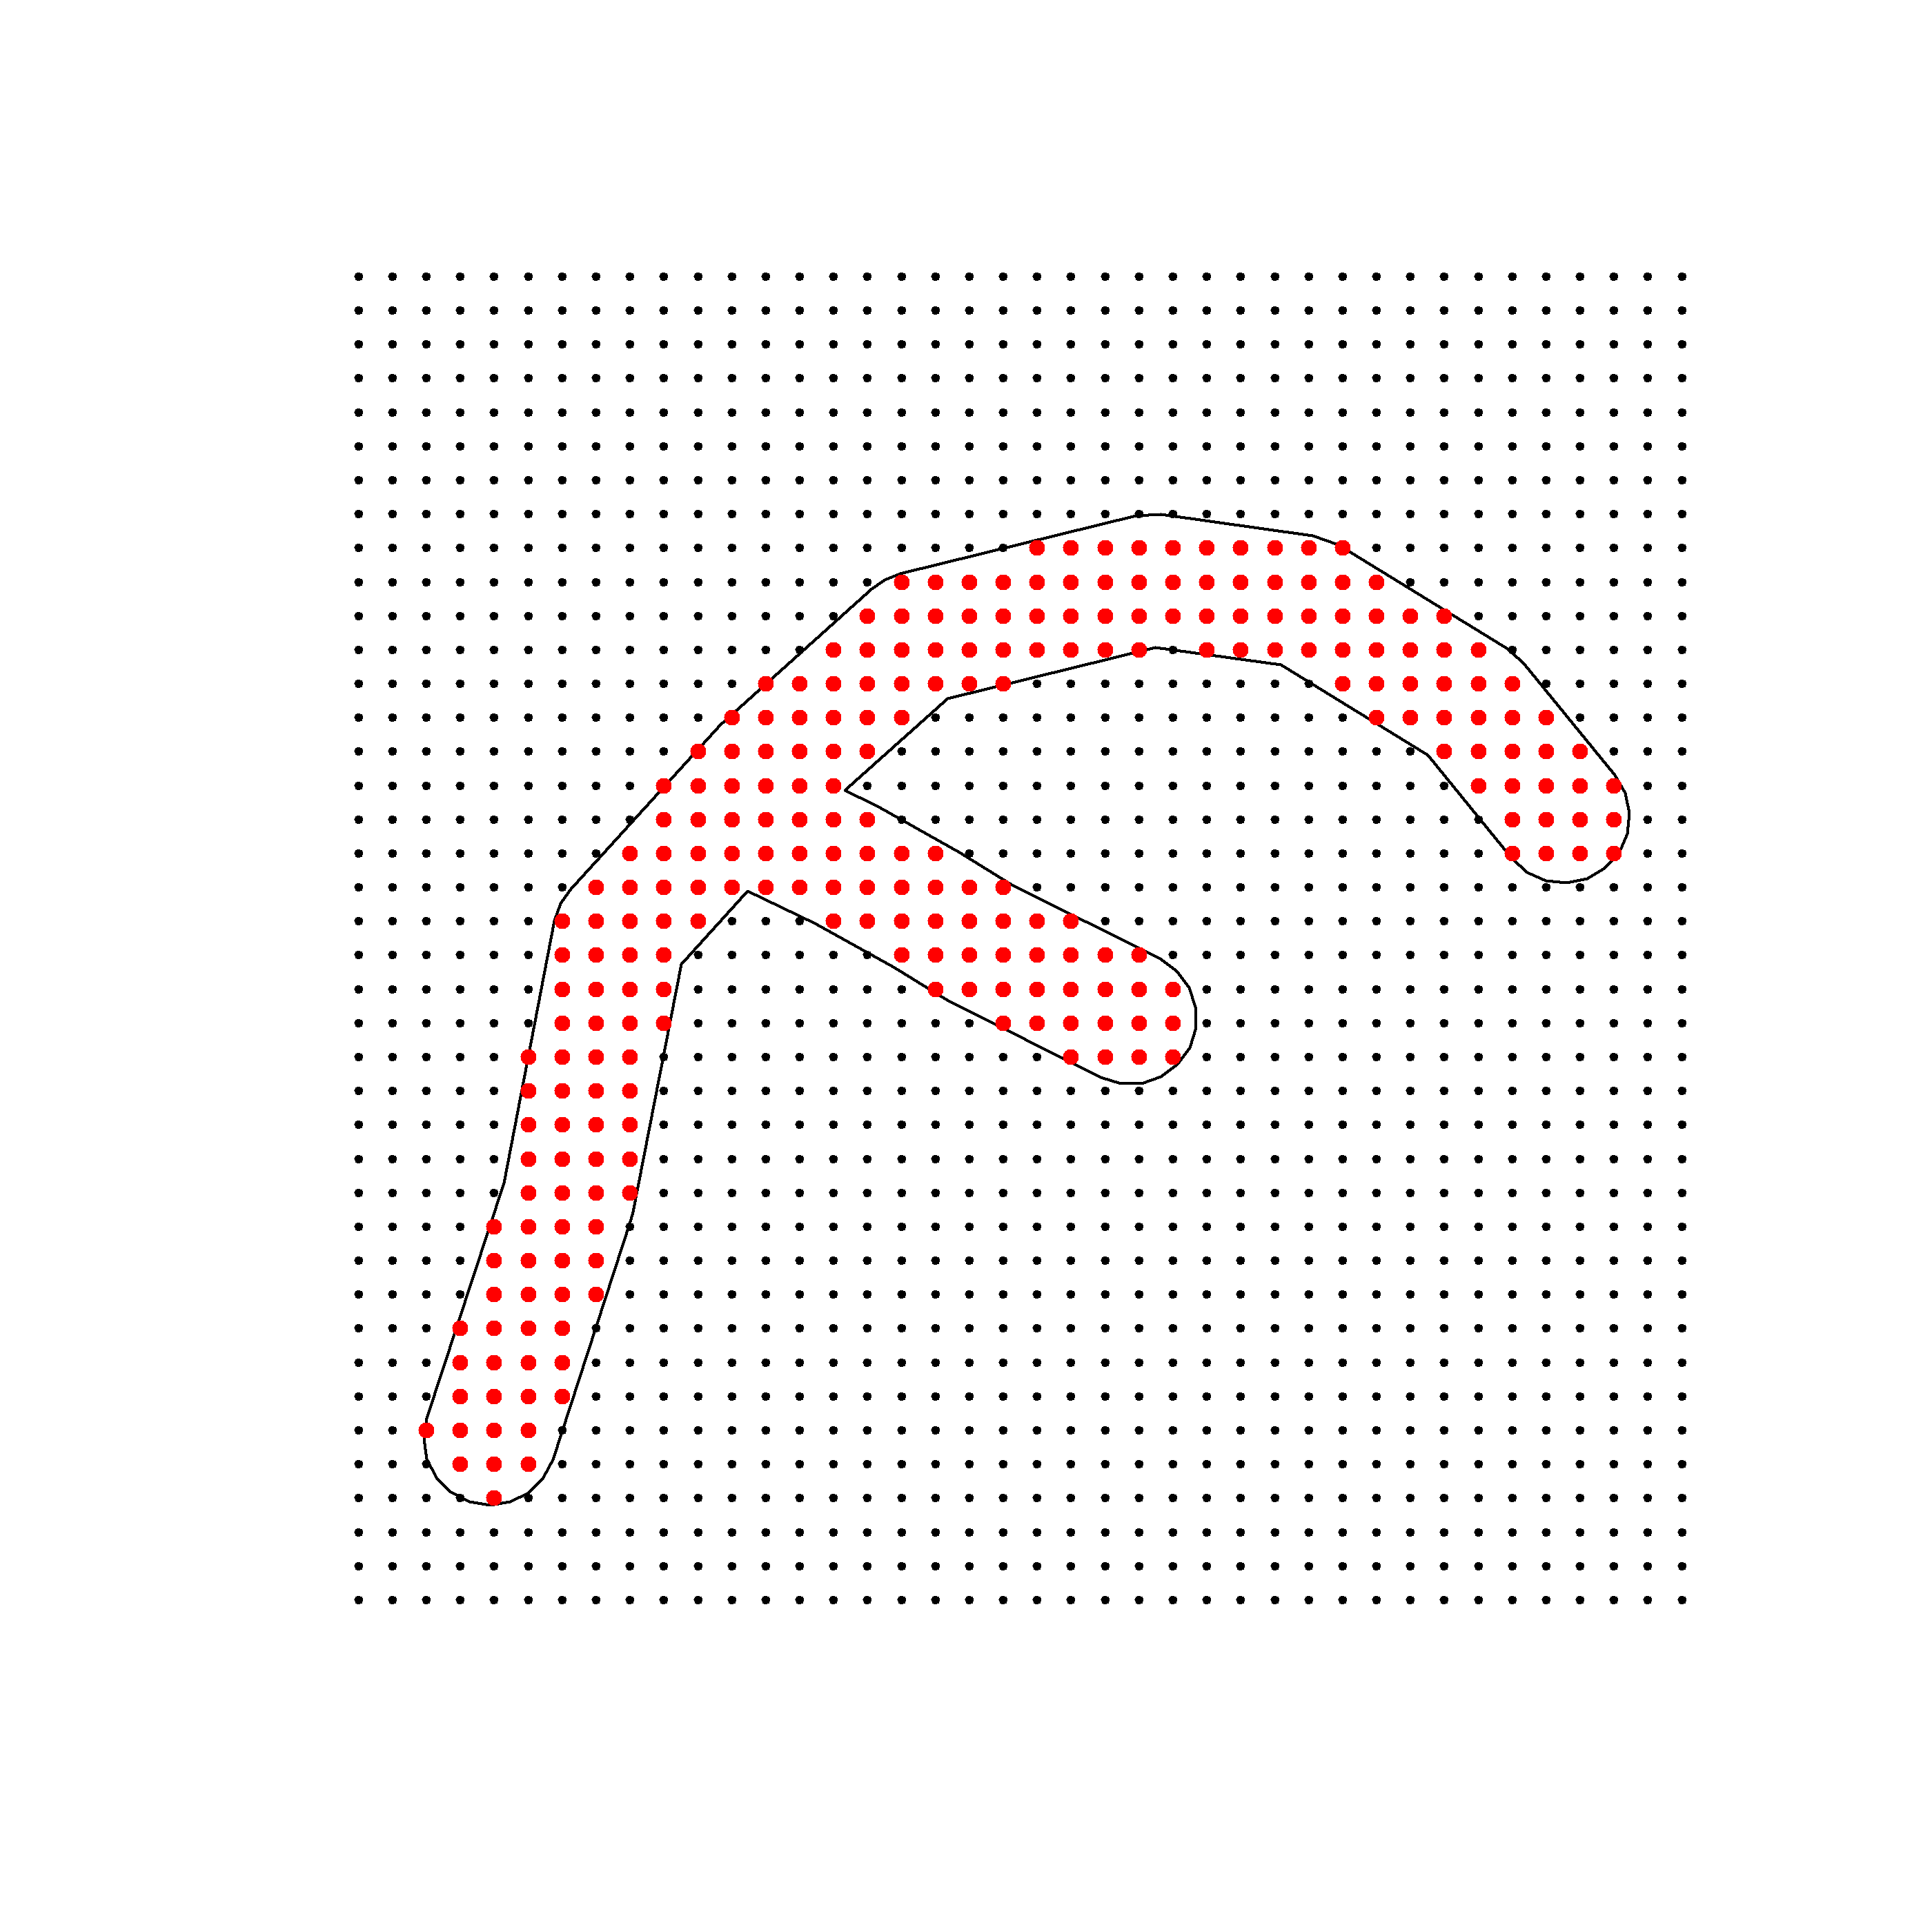
\includegraphics[height=3.25in,width=3.25in]{Ch12-EcolDist/figs/corridor}
\end{center}
\caption{A fake wildlife corridor or reserve. The boundary outlines
  a polygon of suitable habitat surrounded by suburban development.}
\label{ecoldist.fig.corridor}
\end{figure}

In this example, we're not going to estimate parameters of the cost
function. Instead, the point is to compute ordinary Euclidean distance
but restricted by the boundaries of the corridor (or patch geometry in
general) and thus not distance ``as the crow flies.''  To do this, we
imagine that animals will tend to severely avoid leaving the buffered
habitat zone. Therefore, we assign $\mbox{\tt cost}=1$ if a pixel is
within the buffer, and $\mbox{\tt cost} = 10000$ if a pixel is outside
of a buffer. Therefore the cost to move to a neighboring pixel outside
of the buffered area is $5000.5$ compared to the cost of 1 to move to
a neighboring pixel inside the buffer.  With this cost specification,
we can compute the least-cost path distance matrix one time and modify
our likelihood code to accept the distance matrix as input. We give
that likelihood in the package \mbox{\tt scrbook} as the function
\mbox{\tt intlik3edv2}.  We note also that this function accepts a
habitat mask in the form of a vector of 0's
and 1's
that define any potential state-space restrictions. i.e., 1 if
the pixel is an element of the state-space and 0 if it is not, and so
additional modifications to the geometry of the region could be made.
However, in the analysis of this simulated data set, we define the
state-space to be the buffered corridor system.  Here we simulate a
population of $N=200$ individuals in the corridor system and so we
restrict our state-space accordingly for purposes of fitting the
model. However we encourage you to refit the model without the
state-space restriction (for fitting the model only) and then compare
the results.  The code for doing all of this is in the help file for
\mbox{\tt intlik3edv2}, which contains the likelihood function and
sample {\bf R} script (\mbox{\tt ?intlik3edv2}).

{\small
\begin{verbatim}
### Define the cost structure
cost<-rep(NA,nrow(pts))
cost[in.pts==1]<-1      # low cost to move among pixels but not 0
cost[in.pts!=1]<-10000  # high cost

### Stuff costs into a raster
library("raster")
r<-raster(nrows=40,ncols=40)
projection(r)<- "+proj=utm +zone=12 +datum=WGS84"
extent(r)<-c(0-delta/2,10+delta/2,0-delta/2,10+delta/2)
values(r)<-matrix(cost,40,40,byrow=FALSE)

# check what it looks like
plot(r)
points(pts,pch=20,cex=.4)

# compute ecological distances:
library("gdistance")
tr1<-transition(r,transitionFunction=function(x) 1/mean(x),directions=8)
tr1CorrC<-geoCorrection(tr1,type="c",multpl=FALSE,scl=FALSE)
costs1<-costDistance(tr1CorrC,pts)
outD<-as.matrix(costs1)
\end{verbatim}
}

In the next block of code we simulate some data and then fit a model
to the simulated data.  Note that the object \mbox{\tt traps} is
loaded with \mbox{\tt data(fakecorridor)} along with the data which
define the f-shaped patch in
Fig. \ref{ecoldist.fig.corridor}:
{\small
\begin{verbatim}
library(scrbook)
traplocs<-traps$loc
trap.id<-traps$locid
ntraps<-nrow(traplocs)

set.seed(2013)
N<-200
S.possible<- (1:nrow(pts))[in.pts==1]
S.id<-sample(S.possible,N,replace=TRUE)
S<- pts[S.id,]

D<- outD[S.id,trap.id]
eD<- e2dist(S,traplocs)
Dtraps<-outD[trap.id,]

alpha0<- -1.5
sigma<- 1.5
alpha1<- 1/(2*sigma*sigma)
K<-10

probcap<-plogis(alpha0)*exp(-alpha1*D*D)
Y<-matrix(NA,nrow=N,ncol=ntraps)
for(i in 1:nrow(Y)){
 Y[i,]<-rbinom(ntraps,K,probcap[i,])
}
Y<-Y[apply(Y,1,sum)>0,]

frog1<-nlm(intlik3edv2,c(-2.5,2,log(4)),hessian=TRUE,y=Y,K=K,X=traplocs,
            S=pts,D=Dtraps,inpoly=in.pts)
frog2<-nlm(intlik3edv2,c(-2.5,2,log(4)),hessian=TRUE,y=Y,K=K,X=traplocs,
            S=pts,D=Deuclid,inpoly=in.pts)
\end{verbatim}
}

These two models fit, with the correctly specified ecological
distance, constrained by the patch boundaries, and that with the
ordinary (misspecified) Euclidean distance are summarized in Table \ref{rsf.tab.fakecorridor}.
We find little difference between the two models. In
particular, 150 individuals were captured and so truth (the number of
uncaptured individuals) is $\log(n_{0}) = 3.9$.
The correct model produces only a slightly more accurate  estimate, and
it is favored by only 0.7 negative log-likelihood units.
Therefore, for this single instance, the results are not too different.
This is primarily because
 the distance between individuals, and traps that they are likely
to be captured in, is well-approximated by %the
Euclidean distance.


\begin{table}
\centering
\caption{
Summary output of fitting models to simulated data in which movement
is restricted by the habitat corridor shown in
Fig. \ref{ecoldist.fig.corridor}. The two models fitted were those
based on distance  constrained by the corridor boundary
(``constrained'') and a misspecified model based on ordinary Euclidean
distance which is ``as the crow flies'', and cuts through some
boundaries.
See \mbox{\tt ?fakecorridor} for the {\bf R} commands to fit these
models.
}
\begin{tabular}{c|rrrr} \hline \hline
Distance    &  neg. LL &    $\alpha_0$   & $\alpha_1$    & $\log(n_0)$ \\ \hline
constrained & -21.892 &  -1.338 & 0.332 & 4.353 \\
Euclidean   & -21.128 &  -1.307 & 0.382 & 4.212 \\ \hline
\end{tabular}
\label{rsf.tab.fakecorridor}
\end{table}


\section{Ecological Distance and Density Covariates}
\label{chapt.ecoldist.sec.ssed}

Habitat characteristics that affect spatial variation in density can
also affect home range size and movement behavior. For example, a
species that occurs at high density in a forest may be reluctant to
venture from a forest patch into an adjacent field. Thus, even if a
trap placed in a field is located very close to an animal's activity
center, the probability of capture may be very
low. In this case, forest cover is a covariate of
both density and encounter probability,
and we could model it as such by combining the methods described in
this chapter with those described in Chapter~\ref{chapt.state-space}.

To demonstrate, we continue with our analysis of the data shown in
Fig~\ref{state-space.fig.discrete}. Once again, we suppose that density
increases with canopy height, but this time, we also allow
home range size to decrease as density increases. This
commonly-observed phenomenon can be explained by numerous factors such
as intra-specific competition \citep{sillett_etal:2004} or optimal
foraging behavior \citep{tufto_etal:1996,said_servanty:2005}.
%To model
%this effect, we
%introduce the parameter $\theta$, which determines the ``cost'' of
%moving between pixels. If $\theta=0$, then the animal perceives
%distance as Euclidean. If $\theta>0$, then least-cost distance (LCD)
%is greater than than Euclidean distance (ED). In most cases, we would
%not expect,
%or should not even consider the possibility of $\theta<0$ because this
%implies that LCD$<$ED, which would mean that an animal could view
%1000km as 1m. In addition to the fact that this is not biologically
%justifiable, it also suggests that the area of the state-space could
%be infinitely large. Thus, one may want to enforce the constraint that
%$\theta$ is $\geq 0$. See Chapter~\ref{chapt.ecoldist} for
%more details.

A question that arises is: Is it possible to estimate the effect of
the covariate on density ($\bm \beta_1$)
and $\alpha_2$ using standard SCR data? In other words, can we model
spatial variation in density and connectivity at the same time,
using standard SCR data? Currently, it is not possible to
model least-cost distance using \jags~or \secr, so we wrote our own
function, \verb+scrDED+, to fit the model using maximum likelihood. An
example analysis is provided on the help page for the function in our
\R~package \scrbook. We briefly note here that the function requires
the capture history data, the trap locations, and the raster data
formatted using the {\tt raster} package
\citep{hijmans_vanetten:2012}. The linear model for the
intensity parameter $\mu(\mathbf{s}, \beta)$ and the least-cost distance
function $\text{lcd}(\theta)$ are specified using \R's formula interface. A
simple function call is
\begin{verbatim}
fm <- scrDED(y, traplocs=X, den.formula=~elev, dist.formula=~elev,
             rasters=elev.raster)
\end{verbatim}
To assess the possibility of estimating both $\bm \beta$ and $\alpha_2$, we
conducted a small simulation study, generating 500 datasets from the
model with both parameters set to 1, which corresponds to the
conditions described above. The results indicate that it is
possible to estimate both parameters
(Fig~\ref{chapt.ecoldist.fig.simDED}).

\begin{figure}[ht]
\centering
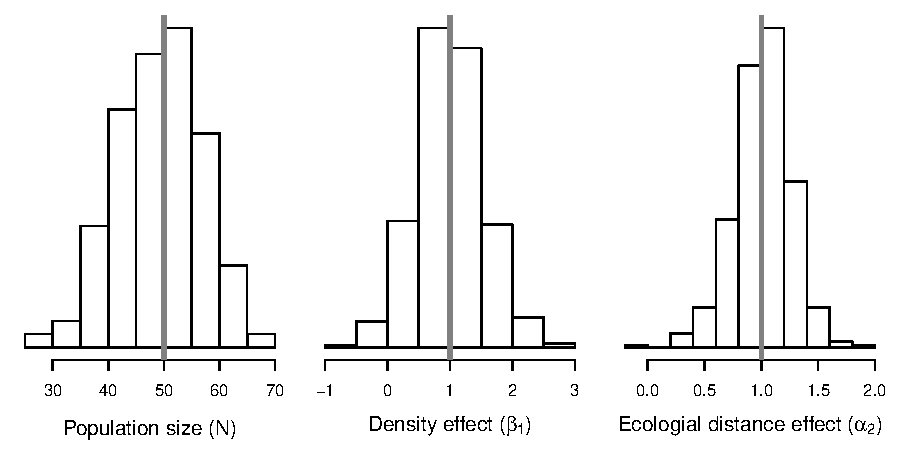
\includegraphics[width=4in,height=2in]{Ch12-EcolDist/figs/scrDEDsim}
\caption{Histograms of parameter estimates from 500 simulations under
  the model in which both density and ecological distance are affected
by the same covariate, canopy height. The vertical lines indicate the
data-generating value.}
\label{chapt.ecoldist.fig.simDED}
\end{figure}



\section{Summary and Outlook}


Almost
all published applications of SCR models to date have been based on
models for the encounter probability that are functions of the
Euclidean distance between individual activity centers and traps. The
obvious limitations of such models are that Euclidean
distance is unaffected by landscape or habitat
structure and implies stationary, isotropic and symmetrical home
ranges. These are standard criticisms of the basic SCR model which we
have seen many times in referee reports, or heard in discussions with
colleagues. However, this should not be seen as criticism
that is inherent to the basic conceptual formulation of SCR models because,
as we have shown here, % that
one can modify the Euclidean distance metric
to accommodate more realistic
formulations of distance that allow for inference to be made about
landscape connectivity, and model ``distance'' as a function of
local habitat characterists. As such, effective distance between individual home
range centers and traps varies depending on the local landscape.

How animals use space and therefore how distance to a trap is
perceived by individuals is not something that can ever be known. We
can only ever conjure up models to describe this phenomenon and fit
those models to limited data on a sample of individuals during a
limited amount of time.  Here we have shown that there is hope to
estimate connectivity parameters
that describe how
animals use space,  from capture-recapture data alone,
thereby allowing  for irregular home range geometry
that is influenced by landscape structure.

In the presence of unctional landscape connectivity, misspecification
of the model by an ordinary SCR model based on Euclidean distance
produces biased estimates of model parameters
 \citep{royle_etal:2012ecol}.
 This is expected because the effect is similar
to failing to model heterogeneity, i.e., if we mis-specify ``model
$M_h$'' \citep{otis_etal:1978} with ``model $M_0$''
\citep{otis_etal:1978} then we will expect to under-estimate $N$. So
the effect of mis-specifying the ecological distance metric with a
standard homogeneous Euclidean distance has the same effect.
In our view, this bias is not really the most important reason to
consider models of ecological distance. Rather, inference about the
structure of ecological distance is fundamental to many problems in
applied and theoretical ecology related to modeling landscape
connectivity, corridor and reserve design, population viability
analysis, gene flow, and other phenomena.  Models based on least-cost
path distance allow investigators to evaluate landscape factors that
influence movement of individuals over the landscape from
non-invasively collected capture-recapture data.  Therefore SCR models
based on ecological distance metrics might aid in understanding
aspects of space usage and movement in animal populations and,
ultimately, in addressing conservation-related problems such as
corridor design.































\chapter{
Integrating Resource Selection
with
Spatial Capture-Recapture
Models}

\markboth{Resource Selection and Space Usage}{}
\label{chapt.rsf}

\vspace{.3in}

\begin{comment}
Up to this point we have developed many variations of SCR models to
describe the observation process.  These included models of the
relationship between encounter probability and distance, and different
types of covariates such as behavioral responses that can affect
detection probability.  Although these different observation models
are immensely useful, they are rather basic in the sense that they
imply simplistic models of how individuals use space (Sec.
\ref{scr0.sec.implied}) and how individuals are distributed in space.
Here,  we generalize the SCR modeling framework to accommodate more
realistic notions of how animals use space.
\end{comment}


In Chapt. \ref{chapt.scr0} we briefly discussed the notion of how
SCR encounter probability models relate to models of space usage.
When using symmetric and stationary encounter probability models, SCR
models imply that space usage is a decreasing function of distance
from an individuals home range center. This is not a very realistic
model in most applications.  In this chapter, we extend SCR
models to incorporate models of resource selection,
such as when
one or more explicit landscape covariates are available which the
investigator believes might affect how individual animals use space
within their home range (this is what \citet{johnson:1980} called {\it
  third-order} selection).  
  
  %XXXX Rahel: I think, out of context third order selection doesnt really mean much; why not briefly state what first and second order selection is? %If I remember right, it's selection on the population level, and selection of home range location within the landscape,right? XXX
  

Our treatment follows
\citet{royle_etal:2012mee} which integrated a standard family of
resource selection models based on auxiliary telemetry data into the
capture-recapture model for encounter probability.
%, and we reproduce
%their case study here in Sec.
%\ref{rsf.chapt.nybears}.
%  The extension of SCR models
%they proposed is consistent with the manner in which classical
%``resource selection function'' (RSF) models \citep{manly_etal:2002}
%or utilization distributions \citep{worton:1989, fieberg:2005,
%  fieberg:2007} are estimated from animal telemetry data.
They  argued that SCR models and resource
selection models \citep{manly_etal:2002} are based on the same basic
underlying model of space usage. The important distinction between SCR
and RSF studies is that, in SCR studies, encounter of individuals is
imperfect (i.e., ``$p<1$'') whereas, with RSF data obtained by
telemetry, encounter is perfect. 
SCR and telemetry data on resource selection can be combined in the
same likelihood by formally recognizing this distinction in the model.  
%We can think of the two as being exactly
%equivalent either if we have a dense array of trapping devices, or if
%our telemetry apparatus is imperfect such as only samples a small area
%of space (this would be consistent with telemetry stations for
%sampling fish which only measure passage at points along a stream or river).

There are two important motives for considering a formal integration
of RSF models with capture-recapture. The first is to integrate models
of resource use by individuals with models of population size or
density. There is relatively little in the literature on this topic,
although \citet{boyce_mcdonald:1999} describe a procedure where (an
estimate of) population size is used to scale resource selection
functions to produce a XXXpopulation?XXX density surface. The second reason is because
this allows for the integration of auxiliary data from telemetry
studies with capture-recapture data.  Telemetry studies are extremely
common in animal ecology for studying movement and resource selection,
and capture-recapture studies frequently involve a simultaneous
telemetry component.  Telemetry data has been widely used in
conjunction with capture-recapture data using standard non-spatial
models.  For example, \citet{white_shenk:2001} and \citet{ivan:2012}
suggested using telemetry data to estimate the probability that an
individual is exposed to capture-recapture sampling. However, their estimator requires
that individuals are telemetry-tagged in proportion to this unknown quantity,
which seems impossible to achieve in many studies. In addition, they
do not directly integrate the telemetry data with the
capture-recapture model so that common parameters are jointly
estimated.  \citet{sollmann_etal:inprepjapplecol} and
\citet{sollmann_etal:2012ecol} used telemetry data to directly inform
the parameter $\sigma$ from the bivariate normal SCR model in order to
improve estimates of density, although these models do not include an
explicit resource selection component.

Formal integration of capture-recapture with telemetry data for the
purposes of modeling resource selection has a number of immediate
benefits. For one, telemetry data provide direct information about
$\sigma$
\citep{sollmann_etal:2012ecol,sollmann_etal:inprepjapplecol}. As a
result, this leads to improved estimates of model parameters, and also
has design consequences (see Sec. \ref{design.sec.outlook}).  In
addition, active resource selection by animals induces a type of
heterogeneity in encounter probability, which is misspecified by
standard SCR encounter probability models. 
% XXX Maybe add some example here; something like: Imagine a camera-trap located some distance $d$ from an individual's activity center in a preferred habitat, say $H1$, and another camera trap the same distance from $s_i$ but in a habitat that is infrequently used by the study species, say $H2$. Then, intuitively, we would expect to photograph $i$ more frequently at the camera trap located in $H1$, simply because it spends more time there. XXX  
As a result, estimates of
population size or density under models that do not account for
resource selection can be biased \citep{royle_etal:2012mee}.  Finally,
because the resource selection model translates directly to a model
for encounter probability for spatial capture-recapture data, the
implication of this is that it allows us to estimate resource
selection model parameters directly from SCR data, i.e., {\it absent}
telemetry data. This fact should broaden the practical relevance of
spatial capture-recapture not just for estimating density, but also
for directly studying movement and resource selection.








\section{A Model of Space Usage}

\label{rsf.sec.rsfmodel}


Assume that the landscape is defined in terms of a discrete raster of
one or more covariates, having the same dimensions and extent.  Let
${\bf x}_{1},\ldots,{\bf x}_{G}$ identify the center coordinates of
$G$ pixels that define a landscape, organized in the 
 matrix ${\bf X}_{G \times 2}$.  Let $C({\bf x})$ denote a
covariate defined for every pixel ${\bf x}$.  We suppose
that individual members of a population wander around space in some
manner related to the covariate $C({\bf x})$.

% XXX  I am not a fan of the "use decision" term.  I think it's just
% use.  You define the movement of an animal from pixel x to x'
% as a decision, which is okay, but that's not what is modeled here...
% R is not really the total number of use decisions, it's just use, right?
% The model has no transition component from pixel x to x'
As a biological matter, use is the outcome of individuals moving
around their home range \citep{hooten_etal:2010}, i.e., where an
individual is at any point in time is the result of some movement
process. However, to understand space usage, it is not necessary to
entertain explicit models of movement, just to observe the outcomes,
and so we don't elaborate further on what could be sensible or useful
models of movement, but we imagine existing methods of hierarchical or
state-space models are suitable for this purpose
\citep{ovaskainen:2004, jonsen_etal:2005, forester_etal:2007,
  ovaskainen_etal:2008, patterson_etal:2008, hooten_etal:2010,
  mcclintock_etal:2012}.  We consider explicit movement models in the
context of SCR models later chapters of this book
(Chapts. \ref{chapt.search-encounter} and \ref{chapt.open}).  Here we
adopt more of a phenomenological formulation of space usage as
follows: If an individual appears in pixel ${\bf x}$ at some instant,  
this is defined as a decision to ``use'' pixel ${\bf
  x}$. 
%XXX RS: This section on truth is a little cryptic. Maybe just needs some re-wording. Plus I agree with reviewer 1 on the use decision terminology XXX
This also induces a definition of ``truth'' -- that is, over
any prescribed time interval, the percentage of time individual spends
in each pixel is theoretically knowable. Or, if we sample some number
of points during that interval, say $R$, 
then the frequency of use decisions is,
 conceivably, observable by some
omnipotent accounting mechanism (e.g., telemetry that doesn't malfunction).
In this
case, let $m_{ij}$ be the {\it true} use frequency of pixel $j$ by
individual $i$ -- i.e., the number of times individual $i$ used pixel
$j$.  We assume the vector of use frequencies ${\bf m}_{i} =
(m_{i1},\ldots,m_{iG})$ has a multinomial distribution:
\[
{\bf m}_{i} \sim \mbox{Multinomial}(R, {\bm \pi}_{i})
\]
where $R = \sum_{j} m_{ij}$ is the total number of ``use decisions''
made by individual $i$ and
\[
 \pi_{ij} = \frac{ \exp( \alpha_{2} C({\bf x}_{j}) ) }{ \sum_{x}
   \exp(\alpha_{2} C({\bf x}))}
\]
This is a standard RSF model \citep{manly_etal:2002} used to model
telemetry data. In particular, this is ``protocol A'' of
\citep{manly_etal:2002} where all available landscape pixels are censused (i.e., known without error), and
used pixels are sampled randomly for each individual.
\begin{comment}
One thing about Manly et al 2002 is that they offer
  numerous ways of modeling resource selection. They offer three
  ``protocols'' (pg 5) describing how used and unused resources are
  sampled. What we are discussing is their protocol A where all
  available resources (pixels) are censused, and used pixels are
  sampled randomly for each individual. They also describe 3 designs
  that vary in whether or not individual level data is collected. I
  think it is just worth being aware of this stuff because everybody
  that talks about RSFs thinks in these terms.
\end{comment}
The parameter $\alpha_2$ is the effect of the
landscape covariate $C({\bf x})$ on the relative probability of
use. Thus, if $\alpha_2$ is positive, the relative probability of use
increases as the covariate increases.

% XXX RS: What about the difficulties of defining 'availability'? It's a big issue in RSF and I think it's worth mentioning. Because it means defining a spatial area that's potentially available to an individual (or a population, depending on the protocoll); and I think it's kind of a spatial problem similar to defining the effective sampled area in traditional CR. Anyway, I think it would be good to at least mention this issue since we're all about the space... XXX

In practice, we don't get to observe $m_{ij}$ for all individuals but,
instead, only for a small subset which we capture and telemeter.  
For the telemetered individuals, we assume
they use resources according to the same RSF model as the population as
a whole.  To extend this model to make it more realistic, and
consistent with the formulation of SCR models, let ${\bf s}$ denote
the center of an individual's home range and let $d_{ij} = ||{\bf
  x}_{j} - {\bf s}_{i}||$ be the distance from the home range center
of individual $i$, ${\bf s}_{i}$, to pixel $j$, ${\bf x}_{j}$. We
modify the space usage model to accommodate that space use will be
concentrated around an individual's home range center:
\begin{equation}
 \pi_{ij} = \frac{ \exp( -\alpha_{1} d_{ij}^{2} +\alpha_{2} C({\bf x}_{j}) ) }
{ \sum_{x} \exp(-\alpha_{1} d_{ij}^{2} +\alpha_{2} C({\bf x}))}
\label{rsf.eq.rsf}
\end{equation}
where $\alpha_1=1/(2\sigma^2)$ describes the rate at which capture
probability XXXX space usage?? XXXX declines as a function of distance from $s_i$.  The parameters
$\alpha_{1}$, $\alpha_{2}$ and the activity centers ${\bf s}$ can be
estimated directly from telemetry data, using standard
likelihood methods based on the multinomial likelihood
\citep{johnson_etal:2008}.
%We note that this form
%(Eq. \ref{rsf.eq.rsf}) arises explicitly as a limiting form of the
%Gaussian process movement model of
%\citet{johnson_etal:2008}. C
%XXX RS: This last sentence is again kind of cryptic without a little more background. Actually, maybe just turning it into 2-3 sentences and being more explicit about what 'which' stands for, would help. Also, I don't know about the 'RSF modeling activities'. Isn't that more a question of how we want to describe our landscape - discrete or continuous? XXX
Sometimes in RSF modeling activities there are continuous
covariates and so the denominator in Eq. \ref{rsf.eq.rsf} involves 
integration over a distribution for the covariate, which is the
conditional intensity of observed point locations in a point process
model. 



The model Eq.~\ref{rsf.eq.rsf} can be understood as a compound model
of space usage governed by distance-based ``availability'' according
to a Gaussian kernel, and also ``use'', conditional on availability
\citep{johnson_etal:2008, forester_etal:2009}.  
% XXX RS: I know I like to be super explicit about things, but these chapters contain so much new information that I think it helps putting examples in. So, maybe somethinge here like: 'In other words, we consider a pixel to be less available to an individual if it is located further away from $s_i$'. The I'd also add in another part about the use, maybe that it is conditional on availability and the RSF? I think this is kind of the core of this model so it wouldn't hurt spending a few more sentences on the two components. XXXXX
Further,
Eq.~\ref{rsf.eq.rsf} resembles standard SCR encounter probability
models that we have used previously, but here the model includes an additional
covariate $C({\bf x})$ (and see Chapt. \ref{chapt.poisson-mn}).  In
particular, under this model for space usage or resource selection, if
we have no covariates at all, or if $\alpha_{2} = 0$, then the
probabilities $\pi_{ij}$ are directly proportional to the SCR model
for encounter probability.  Therefore, setting $\alpha_{2} = 0$, 
the probability of use for pixel $j$ is:
\[
p_{ij} \propto  \exp( -\alpha_{1} d_{ij}^{2}).
\]
% XXXX RS: So far you have only talked about a model for space usage, not encounter prob. in the sense of imperfect detection. It might be worthwhile to point out that you're talking about the shape of the 'detection-with-distance' model (colloquially speaking) but are not yet concerned with the imperfect detection part. I just think otherwise things could get a little confusing for the reader. Or, maybe point out earlier and more clearly the connection between encounter probability and space usage - that one is just a downscaled version (or proportion) of the other. XXX
Clearly, whatever function of distance we use in the RSF model implies
an equivalent model of space usage (Sec. \ref{scr0.sec.implied}) as an
SCR model for encounter probability.  In particular, for whatever
model we choose for $p_{ij}$ in an ordinary SCR model, we can modify
the distance component in the RSF function in Eq. \ref{rsf.eq.rsf}
accordingly to be consistent with that model 
by using whatever function $p_{ij}$ we choose according to
%XXXRS: this sentence is off - too many according to, accordingly, etc. But not sure how to fix it. XXXXX
\[
\pi_{ij} \propto \exp( \log(p_{ij}) + \alpha_{2} C({\bf x}_{j}) )
\]
(see \citet{forester_etal:2009}).  One difference between this
observation model and those that we have considered in previous
chapters is that it includes the normalizing constant $\sum_{x}
\exp(-\alpha_{1} d_{ij}^{2} +\alpha_{2} C({\bf x}_{j}))$, which
ensures that the use distribution is a proper probability density
function. In that sense, the model has the same form as the
multinomial SCR model described in Chapt. \ref{chapt.poisson-mn}
except that, here, the probability is distributed 
%XXXRS: probability density of a location? just so the reader doesnt confuse it with animal density, which also conerns all of S XXXX
over the whole state
space ${\cal S}$, not just the subset of trap locations. In a sense,
we view telemetry data as a perfect sampling of space, equivalent to
having a trap in each pixel, and the number of captures (uses by an
individual) is fixed by design.
%XXX isn't this really similar to the multinomial observation model?
% Andy sez: yes, I edited the material to reflect that point


\citet{royle_etal:2012mee} depict some typical space
usage patterns under the above described model for a single simulated covariate 
(reproduced here in Fig.~\ref{rsf.fig.homeranges}).
\begin{figure}[ht]
\centering
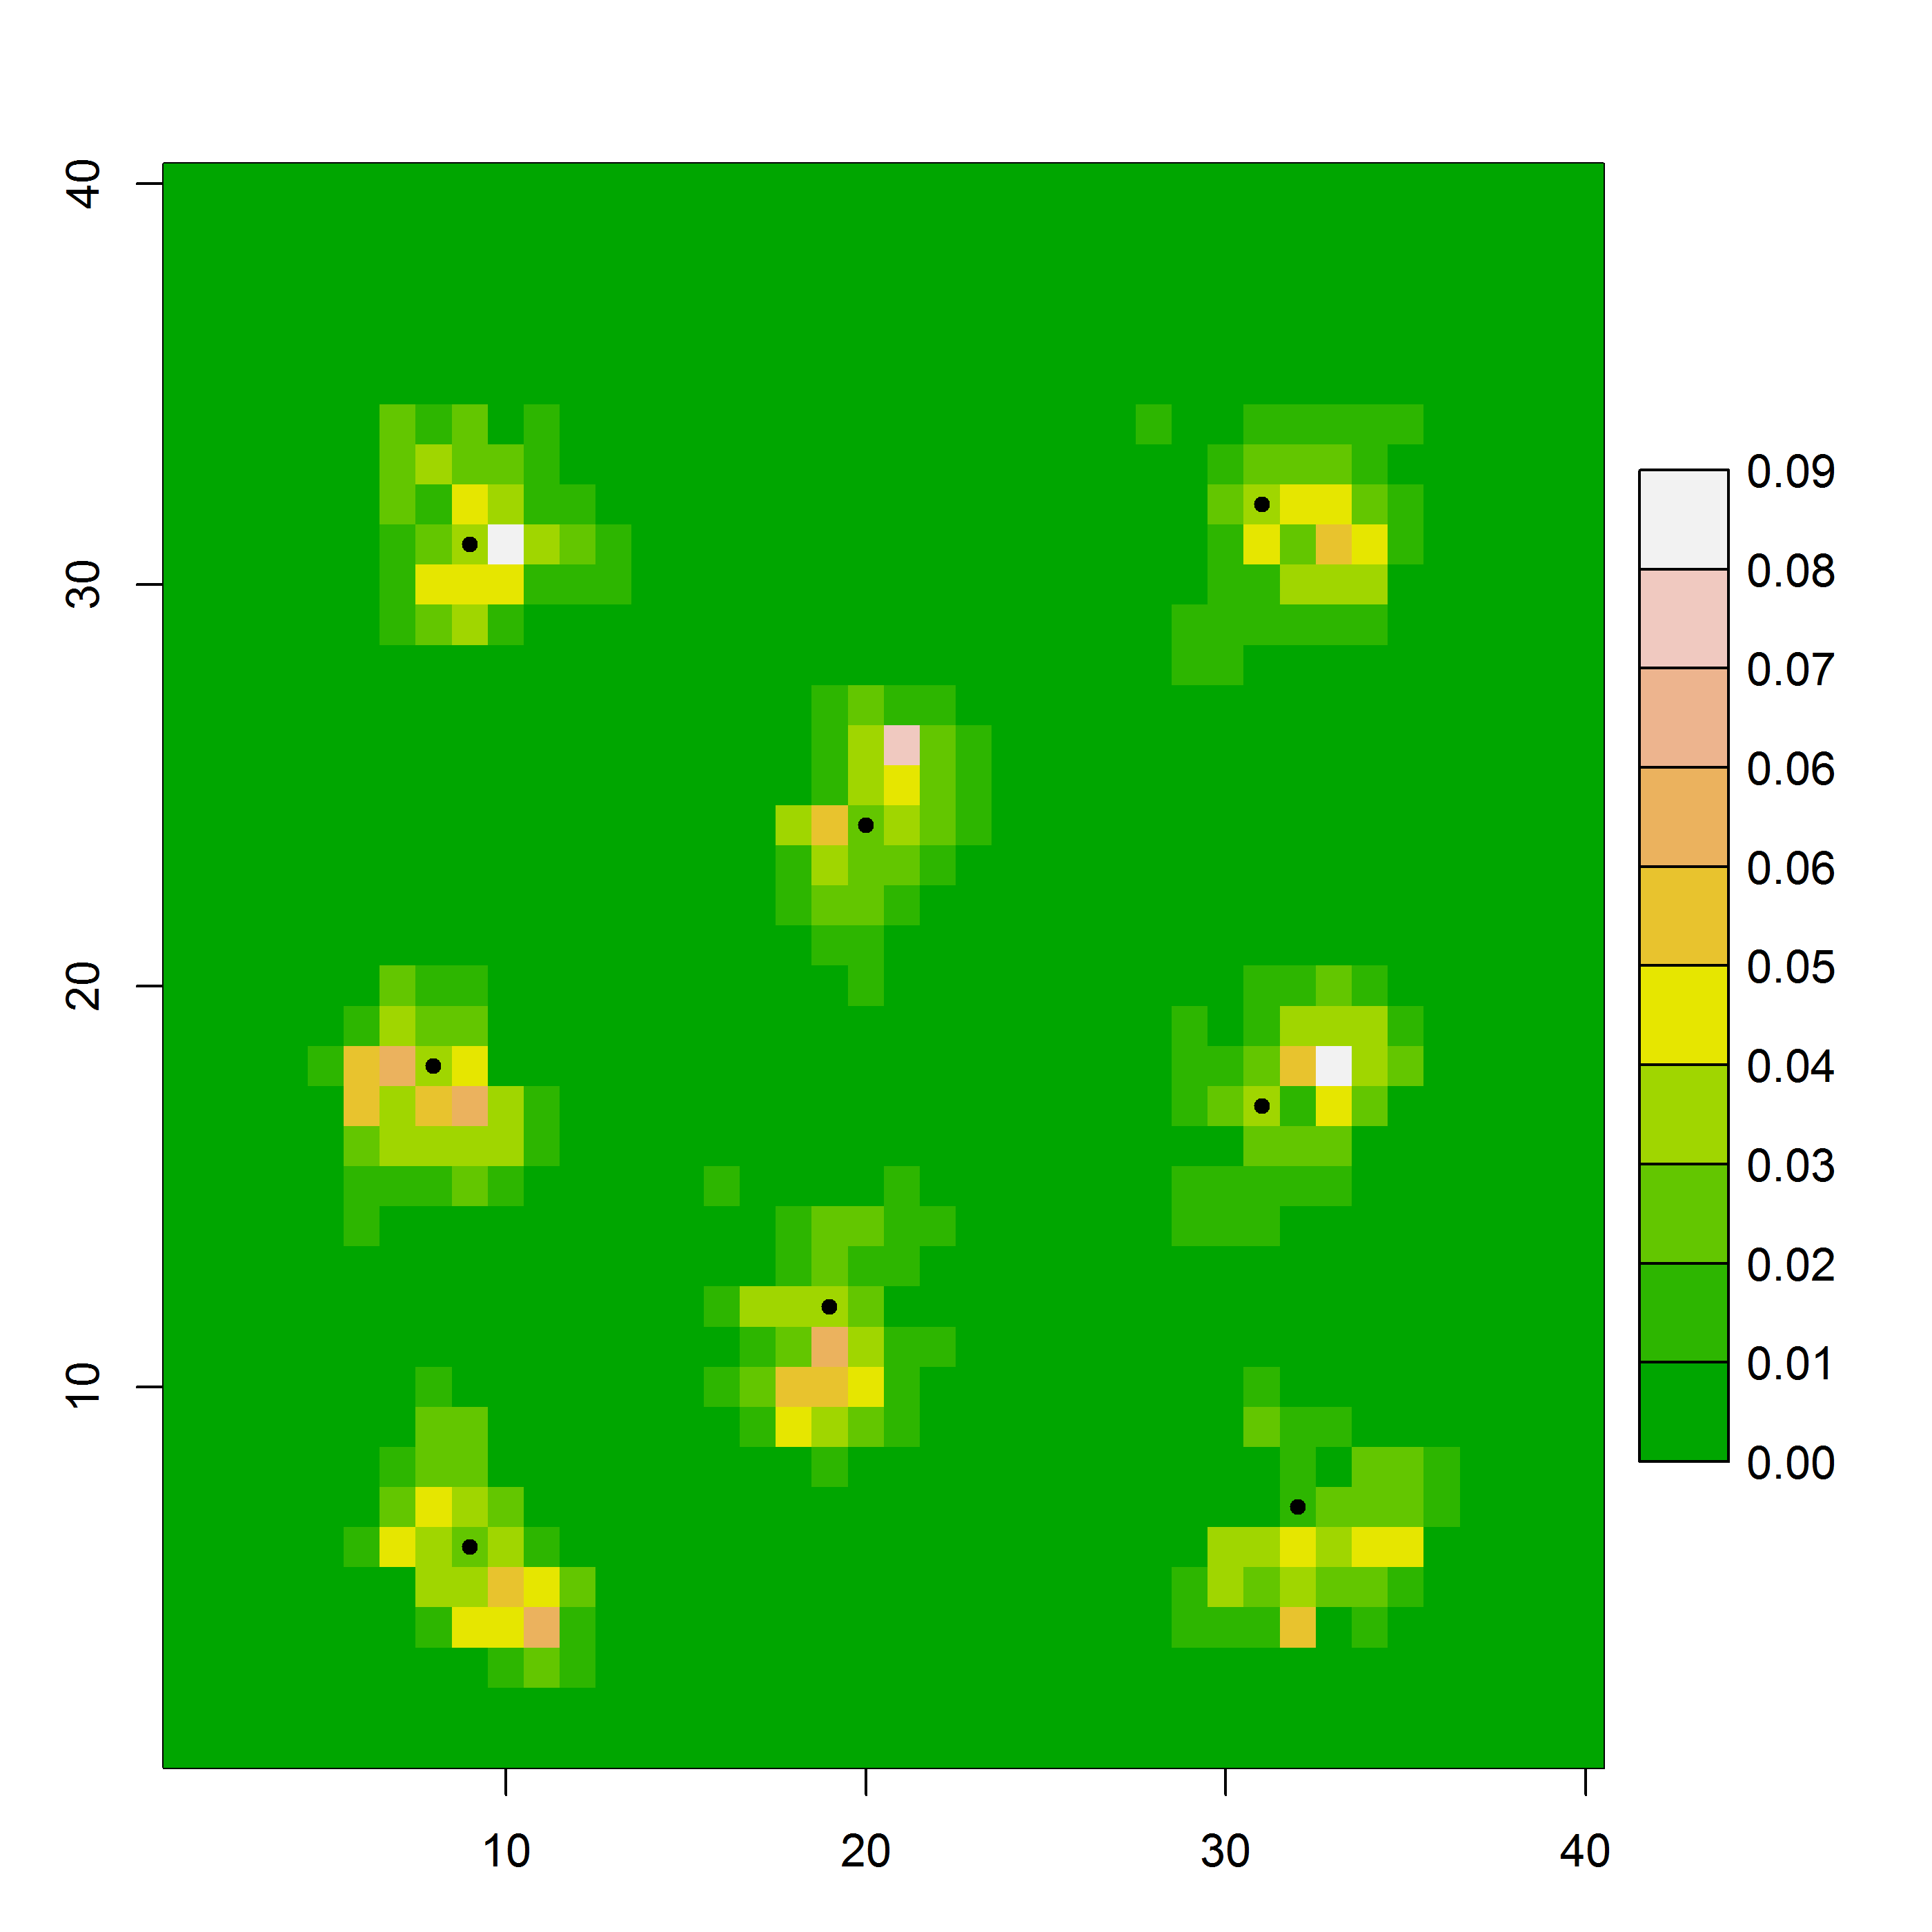
\includegraphics[width=3.5in,height=3.5in]{Ch13-RSF/figs/homeranges8}
\caption{Space usage patterns of 8 individuals under a space usage
  model that contains a single covariate which is shown in
  Fig. \ref{rsf.fig.habitat}. The plotted value is the multinomial
  probability $\pi_{ij}$ for pixel $j$ under the model in Eq. \ref{rsf.eq.rsf}.
}
\label{rsf.fig.homeranges}
\end{figure}
The covariate in this case was simulated using a kriging
model of correlated random noise
with the following {\bf R} commands:
\begin{verbatim}
> set.seed(1234)
> gr <- expand.grid(1:40,1:40)
> Dmat<-as.matrix(dist(gr))
> V <- exp(-Dmat/5)
> C <- t(chol(V))%*%rnorm(1600)
\end{verbatim}
The resulting covariate vector ${\bf C}$ is multi-variate normal with
mean 0 and variance-covariate matrix ${\bf V}$ which, here, has
pariwise correlations which decay exponentially with distance. 
Home ranges shown in Fig.~\ref{rsf.fig.homeranges} were simulated
with $\alpha_{1} =
1/(2\sigma^2)$, with $\sigma = 2$, and the coefficient on $C({\bf x})$
set to $\alpha_{2} = 1$. The resulting space usage densities -- ``home ranges'' -- exhibit clear
non-stationarity in response to the structure of the underlying
covariate, and they are distinctly asymmetrical.  We note that if
$\alpha_{2}$ were set to 0, the 8 home ranges shown here would
be proportional to bivariate normal kernels with $\sigma = 2$.
The commands for the kringing model, and those to produce Fig. \ref{rsf.fig.habitat} are in
the package \mbox{\tt scrbook} (see \mbox{\tt ?RSF$\_$example}).
\begin{figure}[ht]
\centering
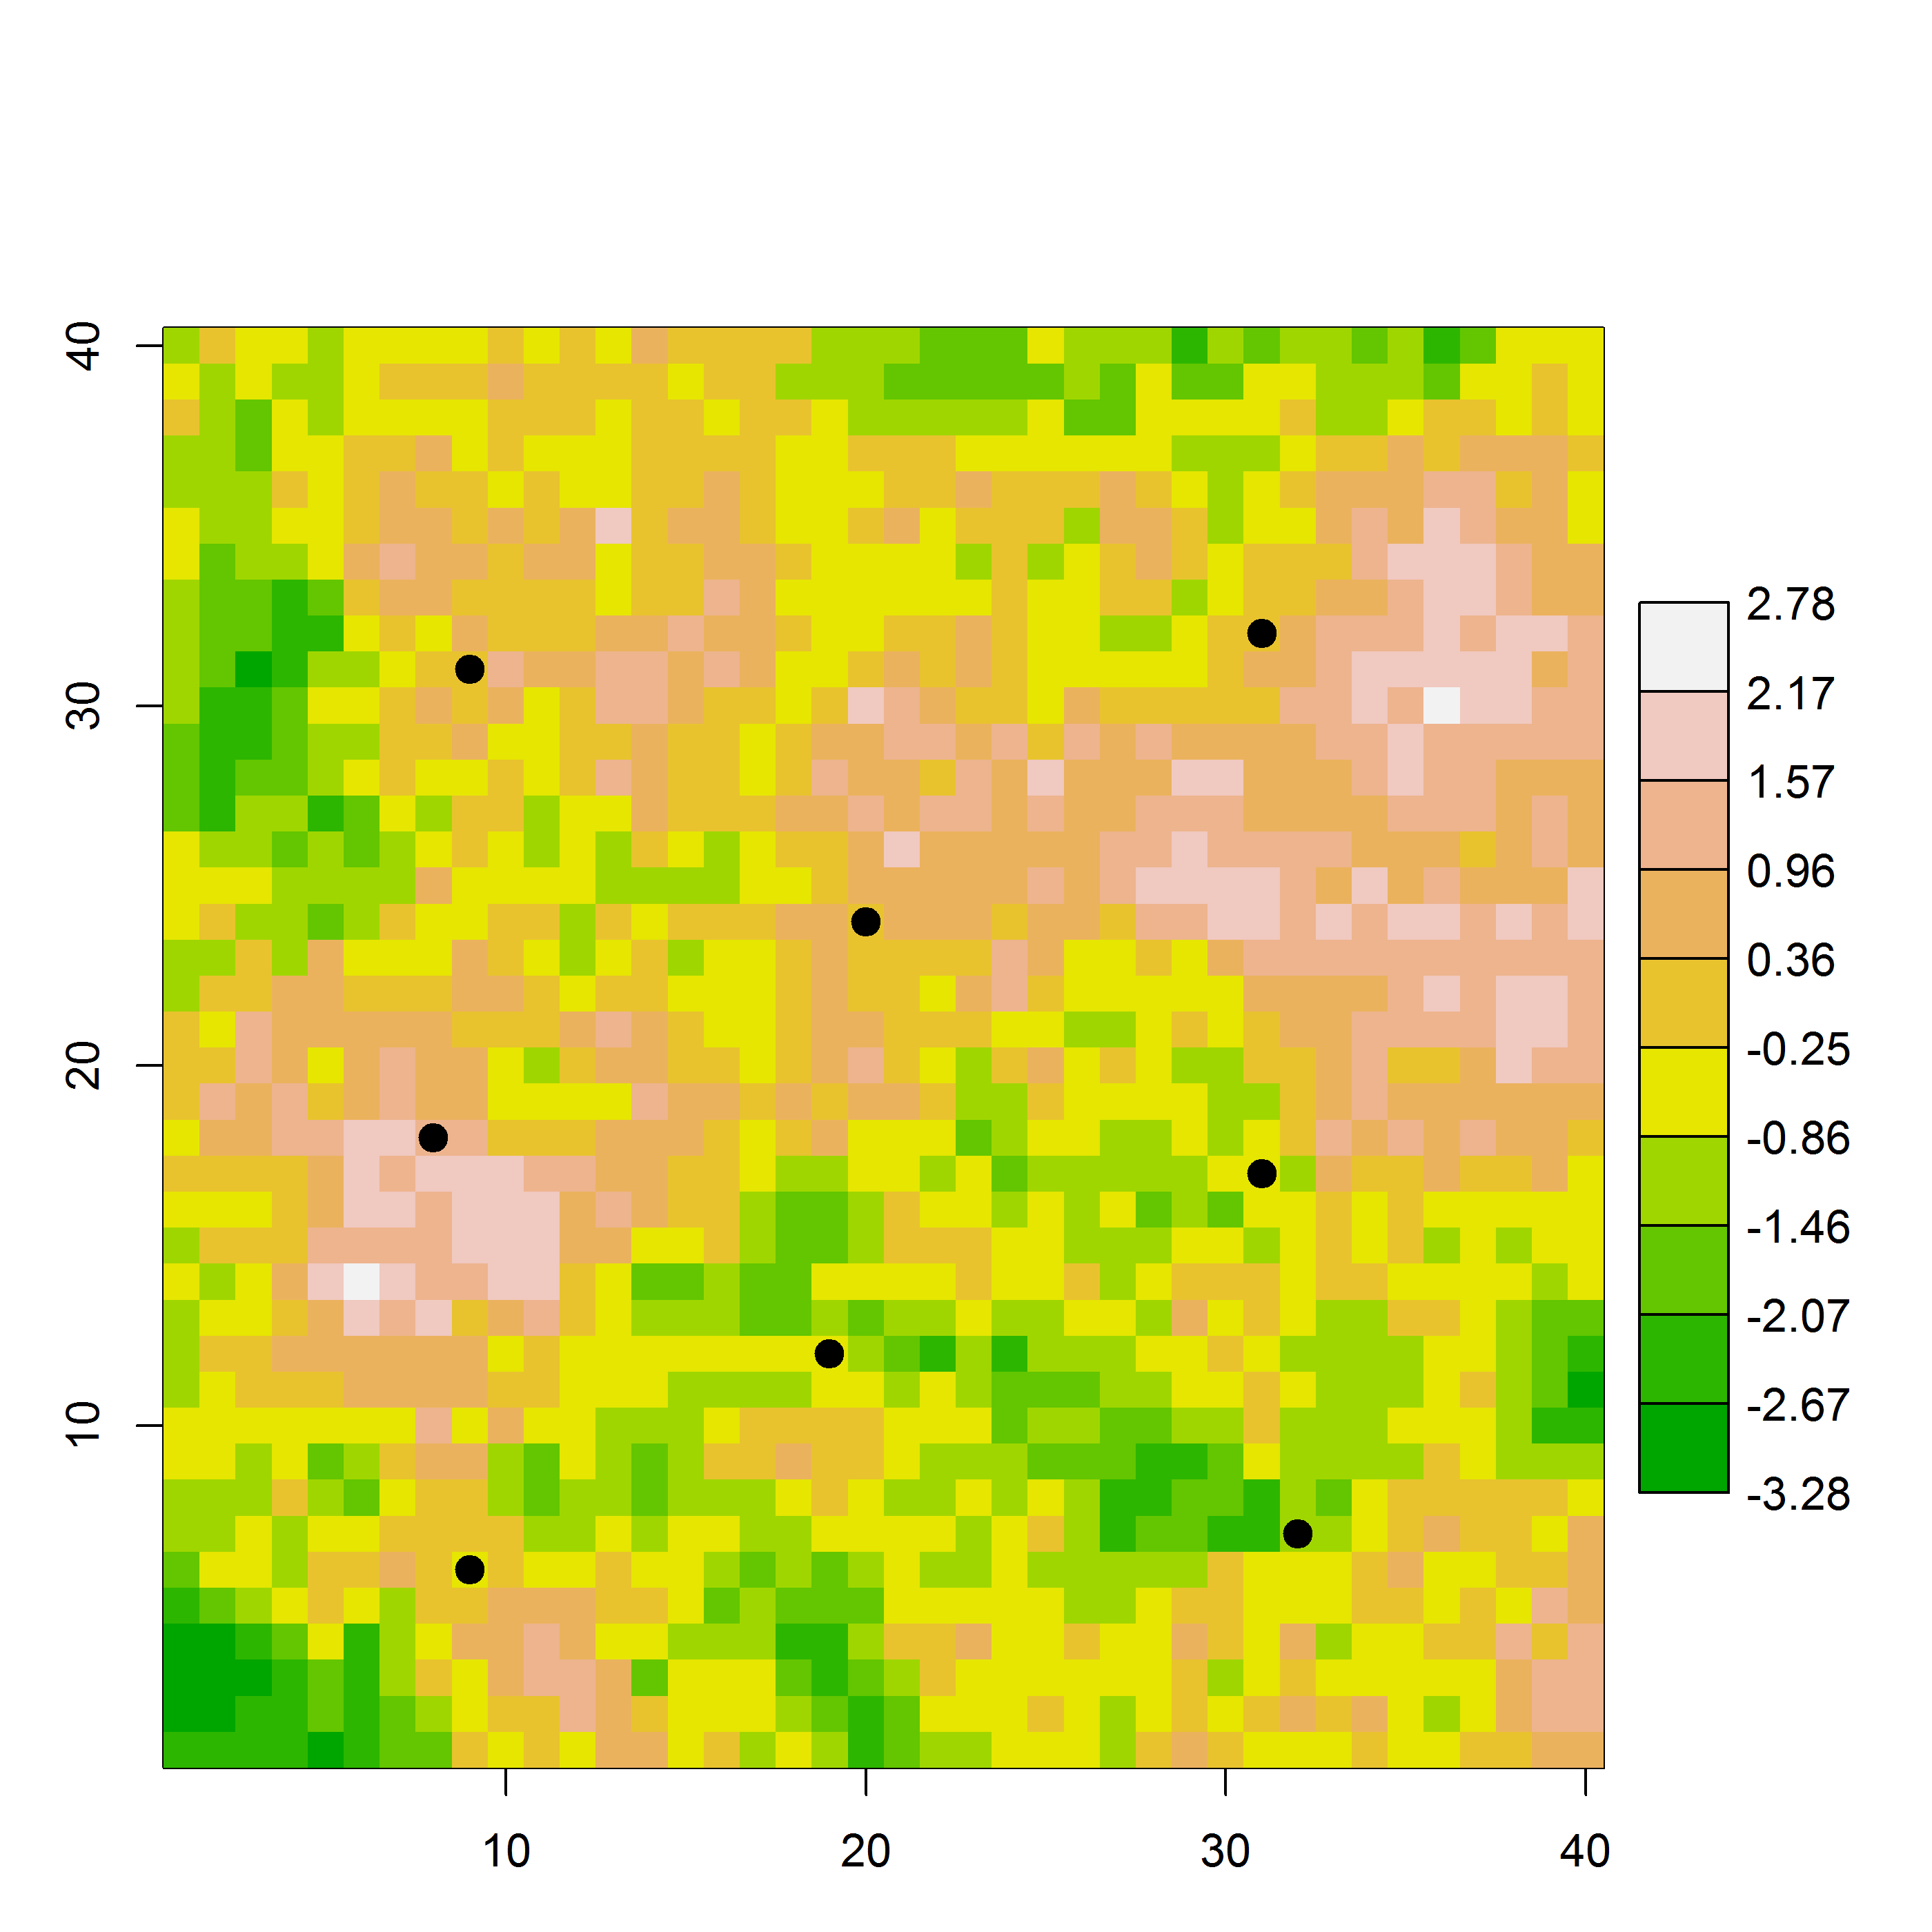
\includegraphics[width=3.15in,height=2.93in]{Ch13-RSF/figs/habitat.png}
\caption{A typical habitat covariate reflecting habitat quality or
  hypothetical utility of the landscape to a species under study. Home
  range centers for 8 individuals are shown with black dots.}
\label{rsf.fig.habitat}
\end{figure}
%XXX RS: I think I'd bring the habitat figure first, then the home ranges XXXX

\subsection{Poisson model of space use}

A natural way to motivate the multinomial model of space usage is to
assume that individuals make a sequence of resource selection
decisions so that the outcomes $m_{ij}$ are {\it
  independent} Poisson random variables:
\[
 m_{ij} \sim \mbox{Poisson}( \lambda_{ij})
\]
where
\[
 \log(\lambda_{ij}) = a_{0} -\alpha_{1} d_{ij}^{2} +  \alpha_{2} C({\bf x}_{j})
\]
In this case, the number of visits to any particular cell is affected
by the covariate $C({\bf x})$ but has a baseline rate, $\exp(a_{0})$,
related to the amount (in an expected value sense) of movement occuring over some time interval.
This is an equivalent model to the multinomial model given previously
in the sense that, if we condition on the total sample size $R = 
\sum_{j} m_{ij}$, then the vector ${\bf m}_{i}$ has a multinomial
distribution with probabilities given by Eq. \ref{rsf.eq.rsf} (see
also Chapt. \ref{chapt.poisson-mn}).  Also note that if use
frequencies are summarized over individuals for each pixel, i.e.,
create the totals $m_{.j} = \sum_i m_{ij}$, then a standard Poisson
regression model for the resulting ``quadrat counts'' is
reasonable. This is ``Design I'' in \citet{manly_etal:2002}.
%XXX maybe say what design I relates to - is it RSF specific or something else?
%%% Richard: can you embellish this a little bit?
% XX RS: Agree: Needs one or two sentences on design 1; also, before you cite Johnson and his levels of selection, then Manly's protocoll A, now design 1. Would be nice to reconcile all those. Maybe a table with the definitions? It just gets messy with 3 different scales/structures for the same problem XXXX

In practice, we never observe ``truth'', i.e., the actual use
frequencies $m_{ij}$. Instead, we observe a sampling XXX sample? XXX of the actual use
outcomes by an individual.  As formulated in
Sec.~\ref{scr0.sec.implied}, we assume a binomial (``random'')
sampling model:
\[
 y_{ij} \sim \mbox{Binomial}(m_{ij}, p_{0}).
\]
We can think of these counts as arising by thinning the underlying
point process (here, aggregated into pixels) where $p_{0}$ is the
thinning rate of the point process.  
% XXX RS: So far we've used point process to describe distribution of s in S. But now you mean the telemetry locations, right? Would make that more explicit XXXXX
In this case, the marginal
distribution of the observed counts $y_{ij}$ is also Poisson but with mean
\[
 \log(\mathbb{E}(y_{ij}))  = \log(p_{0}) + a_{0} -\alpha_{1} d_{ij}^{2} +  \alpha_{2} C({\bf x}_{j}).
\]
Thus, the space-usage model (RSF) for the thinned counts $y_{ij}$ is
the same as the space-usage model for the original variables $m_{ij}$.
This is because if we remove $m_{ij}$ from the conditional model by
summing over its possible values, then the vector ${\bf y}_{i}$ is
{\it also} multinomial with cell probabilities
\[
\pi_{ij} = \frac{\lambda_{ij}}{\sum_{j} \lambda_{ij}}
\]
where any constant (the intercept term $a_0$ and thinning rate
$p_{0}$)
cancel 
from the numerator and denominator. Thus, the underlying multinomial
RSF model applies to the true unobserved count frequencies ${\bf
  m}_{i}$ and also those produced from thinning or sampling, ${\bf
  y}_{i}$.


\section{Integrating Capture-Recapture Data}

The key to combing RSF data with SCR data is 
to note that the Poisson model of space usage given above is 
exactly our Poisson encounter probability model from
Chapt. \ref{chapt.poisson-mn}, but with some arbitrary intercept off-set
related to the 
sampling rate by the telemetry device, and with
a spatial covariate  $C({\bf x})$.
We've used exactly this model for our SCR data (Chapt. \ref{chapt.covariates}), but with a different intercept,
$\alpha_{0}$, unrelated to the intercept of the Poisson use model
for telemetry described above but, rather, to the efficiency of the capture-recapture
encounter device. 
In other words, we view camera traps (or other devices) located in
some pixel ${\bf x}$ (or multiple pixels) as being equivalent to being able to turn on a
type of (less perfect) telemetry device only in that pixel.
%result of some thinning of the ``true'' space usage outcomes.
%In other words, imagine that we have a sampling device, such as a
%camera trap, in {\it every} pixel. If the device operates continually
%then it functions similar to a telemetry instrument in the sense that
%we can observe an individual in {\it any} pixel. But, given that 
%Given that real sampling devices
% operate imperfectly, intermittently, or do not expose the
%entire area of each pixel, then a reasonable model for this imperfect
%observation is the ``thinned'' binomial model given above, but with a
%different 
%intercept, say 
%representing the sampling
%effectiveness of the device, what we've called the baseline encounter
%rate in previous chapters. 
Therefore, 
data from a camera trapping are Poisson random variables 
for every pixel $j$ where a trap is located:
\[
y_{ij}|{\bf s}_{i} \sim \mbox{Poisson}( \lambda_{ij})
\]
with 
\[
 \log(\lambda_{ij}) =  \alpha_{0} -\alpha_{1}
 d_{ij}^{2} +  \alpha_{2} C({\bf x}_{j}).
\]
The parameters $\alpha_{1}$ and $\alpha_{2}$ are shared with the
multinomial model for the telemetry data.

Alternatively, 
the SCR study can produce binary 
encounters depending on the type of sampling being done,
where $y_{ij} = 1$ if the individual $i$ visited
the pixel containing a trap and was detected, then we imagine that
$y_{ij}$ is related to the latent variable $m_{ij}$ being the event
$m_{ij}>0$, which occurs with probability
\begin{equation}
 p_{ij} = 1-\exp(- \lambda_{ij})
\label{rsf.eq.cloglog}
\end{equation}
%We combine the constants so that $\alpha_{0} = \log(\lambda_{0}) + a_{0}$
%is the baseline encounter rate which includes the constant intensity
%of use by the individual and also the baseline rate of detection,
%conditional on use.  The Bernoulli observation model implies that the
and then the observed encounter frequencies for individual $i$ and trap $j$, from
sampling over $K$ occassions are binomial:
\[
 y_{ij}|{\bf s}_{i} \sim \mbox{Binomial}(K, p_{ij}) 
\]

A key point here is that if resource selection is happening, then it
appears as a covariate on encounter rate (or encounter
probability) in the same way as ordinary covariates which were discussed in
Chapt. \ref{chapt.covariates}.


\subsection{The Joint RSF/SCR Likelihood}

To construct the likelihood for SCR data when we have 
direct information on space usage
from telemetry data, we regard the two samples (SCR and RSF) as
independent of one another, and we 
 form the likelihood for each set of observations as a function
of the same underlying parameters. The joint likelihood then is the
product of the two components. 

In particular, let ${\cal L}_{scr}(\alpha_{0}, \alpha_{1}, \alpha_{2}, N;{\bf y})$
be the likelihood for the SCR data in terms of the basic encounter
probability parameters and the total (unknown) population size $N$,
and let ${\cal L}_{rsf}(\alpha_{1},\alpha_{2}; {\bf m})$ be the
likelihood for the RSF data based on telemetry which, because the
sample size of telemetered individuals is fixed, does not depend on $N$.
Assuming independence of the two datasets, the
joint likelihood is the product of these two pieces:
\[
{\cal L}_{rsf+scr}(\alpha_{0},\alpha_{1},\alpha_{2},N; {\bf y},{\bf
  m})  =
{\cal L}_{scr}(\alpha_{0}, \alpha_{1}, \alpha_{2}, N;{\bf y})
\times
{\cal L}_{rsf}(\alpha_{1},\alpha_{2}; {\bf m}),
\]
where the ${\cal L}_{scr}$ is the standard integrated likelihood
(Chapt. \ref{chapt.mle}), and the RSF likelihood contribution is the
multinomial telemetry likelihood having cell probabilities
Eq. \ref{rsf.eq.rsf}.  The {\bf R} code for this 
%XXX to maximize the joint likelihood? or for what? XXX 
was given in the
supplement to \citet{royle_etal:2012mee}, and we include a version of
this in the \mbox{\tt scrbook} package, see \mbox{\tt ?intlik3rsf},
which also shows how to simulate data and fit the combined SCR+RSF
model.

%XXX a lot of our book is from papers, but this section below sounds
%particularly like we didn't try.  I revised it a bit, hope you think it's okay
%% Andy sez: Beth -- thanks for that, I think this is good. I might
%% micro-edit it.

\section{SW  New York Black Bear Study}
\label{rsf.chapt.nybears}

\citet{royle_etal:2012mee} applied the integrated SCR+RSF model to
data from a study of black bears ({\it Ursus americanus})
in a region of approximately 4,600
km$^2$ in southwestern New York \citep{sun:2013}\footnote{This is
different from our Fort Drum bear study data set which we've analyzed
in previous chapters}.  The data can be loaded from the \mbox{\tt scrbook}
library with the command \mbox{\tt data(nybears)}.
We reproduce the findings of \citet{royle_etal:2012mee} in this section.

The data are based on a noninvasive genetic capture-recapture study
using 103 hair snares in June and July, 2011.  Hair snares were baited
and scented and checked weekly for hair \citep{sun:2013}.  The study
yielded relatively sparse encounter histories
 of 33 individuals with a total of 14 recaptures (27
individuals captured 1 time only.
% Extra trap recaptures included  %XXX what is an extra trap recap?
%3 individuals captured in 2 traps, 1 individual in each of 3 and 4
%traps).  
Telemetry data were collected on 3 telemetry-collared individuals, which produced
locations for each bear approximately once per hour.  We 
thinned these data to once per 10 hours to produce movement outcomes that might
be more independent. This produced 195 telemetry locations used in the
RSF component of the model.  Elevation was used as the covariate for this 
model, a standardized version of which is shown in
Fig. \ref{fig.elevation} along with the locations of each
capture at hair snare sites.  


\begin{figure}[ht]
\centering
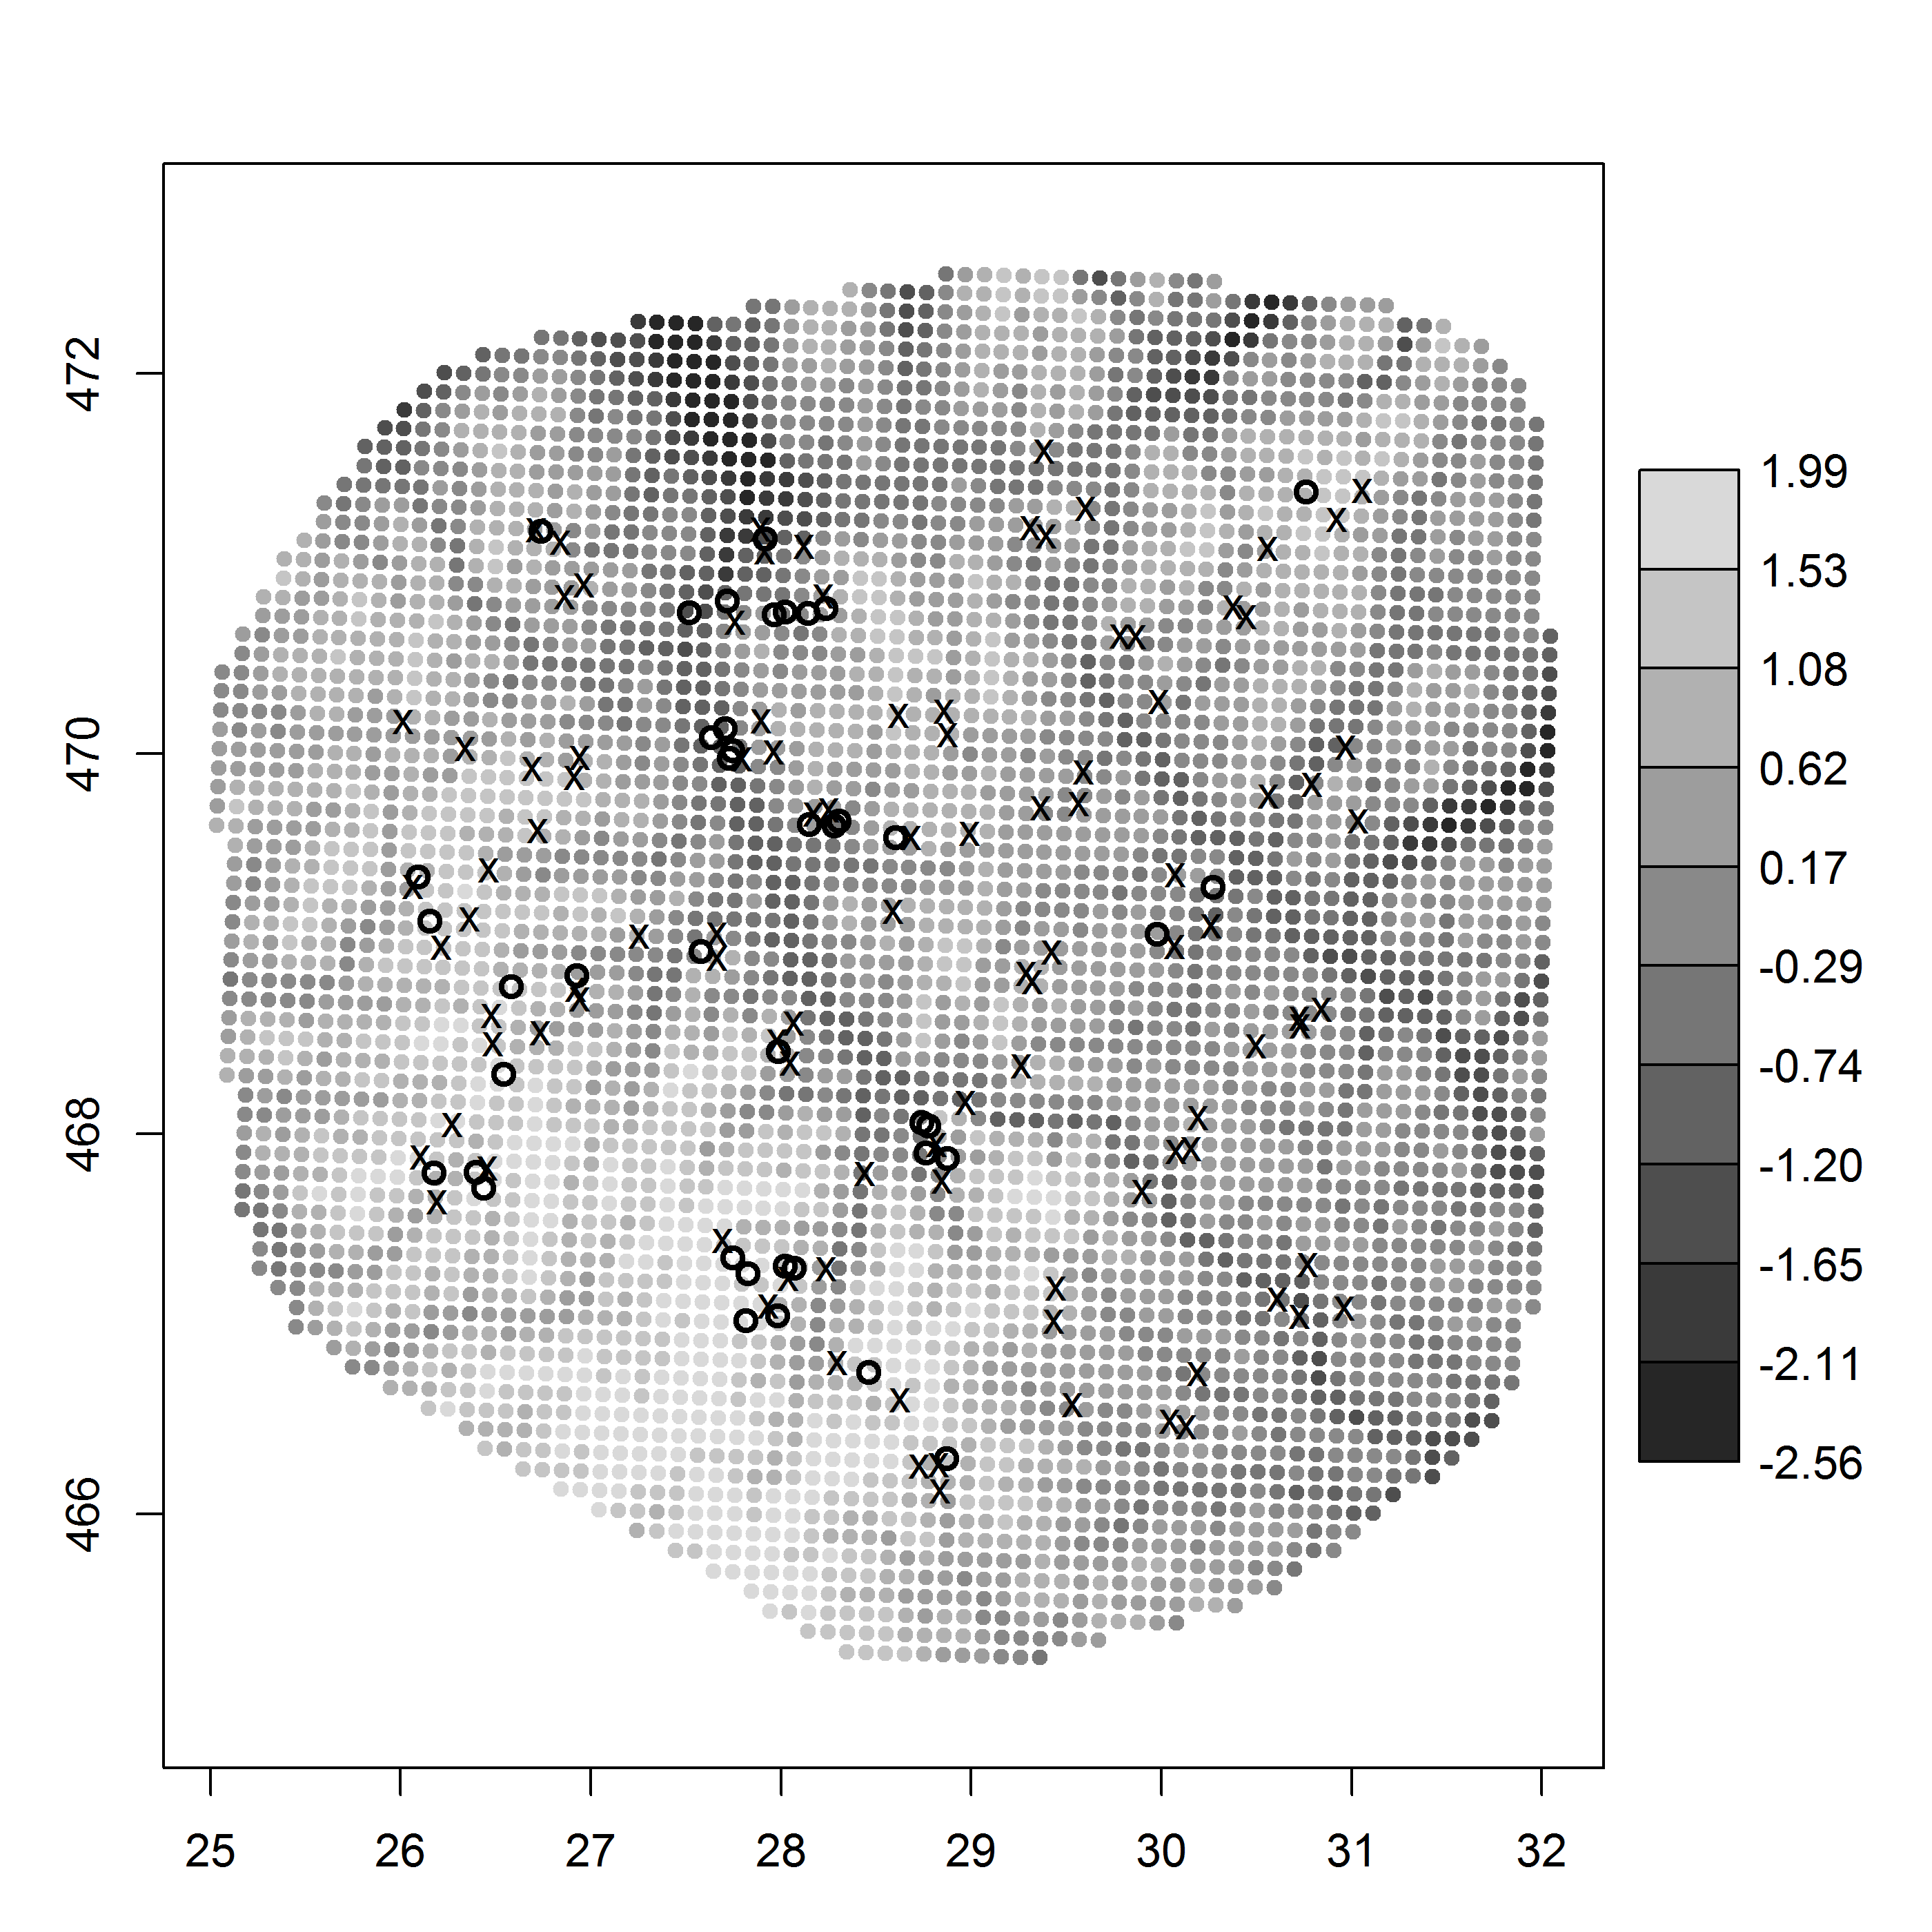
\includegraphics[width=3.25in,height=3.25in]{Ch13-RSF/figs/elev_captures_bw.png}
\caption{
Elevation (standardized), hair snare locations (indicated by ``$x$'') and location
of bear captures (open circles).
Multiple captures at a trap location are offset by adding
random noise.
}
\label{fig.elevation}
\end{figure}

%XXXX RS: I think this figure needs some work; symbols are difficult to distinguish. XXXX

There are a number of models that could be fitted to these data based on
the combination of SCR and RSF data as well as the elevation covariate.  
The models fit here are
 based on the Gaussian hazard trap encounter/space usage model,
including an ordinary SCR model with no covariates or telemetry data,
the SCR model with elevation affecting either $\lambda_{0}$ or density
$D({\bf x})$ (Chapt. \ref{chapt.state-space}), and models that use
telemetry data.  The 6 models fitted were:
\begin{itemize}
\item[] Model 1,  SCR: ordinary SCR model
\item[] Model 2, SCR+p(C): ordinary SCR model with elevation as a
  covariate on baseline encounter probability $\lambda_{0}$.
\item[] Model 3, SCR+D(C): ordinary SCR model with elevation as a
  covariate on density only.
\item[] Model 4, SCR+p(C)+D(C): ordinary SCR model with elevation as
  a covariate on both baseline encounter probability and density.
\item[] Model 5, SCR+p(C)+RSF: SCR model including data from 3
  telemetered individuals.
\item[] Model 6, SCR+p(C)+RSF+D(C): SCR model including telemetered
  individuals and with elevation as a covariate on density.
\end{itemize}
It is tempting to want to compare these different models by AIC but,
because models 5 and 6 involve additional data, they cannot be
compared with models 1-4.  Parameter estimates for the six models are
given in Table \ref{tab.nyresults} (reproduced from
\citet{royle_etal:2012mee}, see also the help file \mbox{\tt
  ?nybears}).

By looking at Table \ref{tab.nyresults}, it is clear based on the
negative log likelihood for just Models 1-4, that those containing an
elevation effect on density are preferred (Model 3 and 4).  The
parameter estimates indicate a positive effect of elevation on
density, which seems to be consistent with the raw capture data shown
in Fig. \ref{fig.elevation}.  Despite this strong effect
of elevation, the estimates of $N$ under each of these models only
ranged from $93 - 103$ bears for the 4600 km$^2$ state-space.
%XXX RS: So density is pretty constant across models? XXX
  If we
consider not just density, but space usage (i.e., looking at the
parameter $\alpha_2$), the effect of elevation is negative.  Thus, elevation, appears to affect density and space usage
differently.  It was suggested that density operates at the
second-order scale of resource selection and ``....is largely related
to the spacing of individuals and their associated home ranges across
the landscape.  On the other hand, our RSF was defined based on
selection of resources within the home range (third-order).''
\citep{royle_etal:2012mee} 
%XXXX RS: Since you bring up second-order resource selection here, the different orders def. need to be defined earlier on XXX
The positive effect of density on elevation
is consistent with some other studies XXX on black bears? XXXX \citep[e.g.][]{frary_etal:2011},
and the negative effect of elevation on space usage can be attributed to
seasonal variation in food availability, usage of corridors, or
environmental conditions.


Models 5 and 6 include the additional telemetry data, thus the
negative log-likelihoods are not directly comparable to the first 4
models, but we can still make a few important observations.  First is
that the parameter estimates under these two models are consistent
with Model 4 in that elevation had a strong effect on both density and
space usage.  In comparing models 5 and 6, the latter model which
includes elevation as an effect on density reduces the negative
log-likelihood by 5 units.  Additionally, including the telemetry data
reduces the standard errors (SE) of the density and space usage
parameters and as we would expect, the incorporation of telemetry data
also reduces the SE for $\sigma$.  The increased precision for the
estimated population size ($N$) is negligible with the use of
telemetry data in this case.  However, that may be different if more
telemetry information were available.  Model 6 (SCR+p(C)+RSF+D(C)),
was used to produce maps of density (Fig. \ref{fig.density}) and space
usage (Fig. \ref{fig.spaceusage}) showing the effect of elevation on
both components of the model.  The map of space usage shows the
relative probability of using a pixel ${\bf x}$ relative to one having
the mean elevation, given a constant distance to the individual's
activity center.
 %XXXX is that a correct interpretation of what you did?


\begin{comment}

XXX Beth: I rewrote all of this above  
XXX you can put it all back in and take my stuff out if you want

{\bf XXXXXXXX below is exactly plagarized from the paper XXXXXXXXXXXX}
Looking at  models 1-4, which do not use the telemetry observations,
models in which elevation effects density are preferred, and we see a
a large positive response to elevation, which is apparent in
consistent with the visual pattern apparent in
Fig. \ref{fig.elevation} (more captures at higher elevations).
Conversely,
there is a negative effect of elevation on
space usage (the parameter $\alpha_{2}$).
The estimate of $N$ for the 4600 km$^2$ state-space, based on the best
model is about 103 bears $(\exp(4.25)+33)$.
In the two models that include the additional telemetry data, a couple
points stand out: Clearly the elevation effect on density is
important, reducing the negative log-likelihood by 5 units. The effect
of elevation on density and space usage are roughly consistent with
Model 4 which did not use telemetry data. Furthermore, the standard
errors (SE) of those two parameter estimates are reduced considerably
when the model uses telemetry data, as is the SE for estimating
$\log(\sigma)$.  The SE for estimating $\log(n_{0})$ is only improved
incrementally compared to the models without telemetry data.  We used
the best model, \mbox{\tt SCR+p(C)+RSF+D(C)}, to produce a map of
density (Fig. \ref{fig.density}) which shows clearly the pattern
induced by elevation. We also produced a map
(Fig. \ref{fig.spaceusage}) to illustrate the effect of elevation on
space usage. This shows the relative probability of using a pixel
${\bf x}$ relative to one of mean elevation, and of the same distance
from an individual's activity center.
% remind people how to compute "the relative prob of using pixel x XXXX
%The cool thing about these models is we can make pretty
%multi-colored maps of things.  A map of density under the
%model is shown in fig. \ref{fig.density}.  A map of space usage in
%terms of the relative probability of using pixel $x$ relative to the
%average pixel is shown in Fig. \ref{fig.spaceusage}.

\end{comment}

\begin{comment}
I computed the MLE of N and the SE using a delta approximation as
follows: The MEE paper has log(n0) and the se of log(n0) which is not informative.
> logn0<-c(4.140,4.110,4.114,4.255,3.884,4.028)
> sev<- c(0.366,0.362,0.358,0.377,0.363, 0.366)
> exp(logn0)+33
[1]  95.80282  93.94672  94.19099 103.45682  81.61830  89.14850
> sev*exp(logn0)
[1] 22.98583 22.06271 21.90638 26.56222 17.64844 20.55035
\end{comment}

%XXX RS: Table seems to wide and seems to have a different format from rest of the book (vertical line, more horizontal lines ) XXX
\begin{table}
\centering
\caption{
Summary of model-fitting results for the black bear study. Parameter
estimates are for the intercept ($\alpha_{0}$), logarithm of $\sigma$,
the
scale parameter of the Gaussian hazard encounter model, 
 $\beta$ is the coefficient of elevation on density, and the total
 population size $N$ of the state-space. Standard errors
 rae in parentheses.
The SCR data are based on $n=33$ individuals, and the telemetry data
are based on 3 individuals. 
}
\begin{tabular}{c|rrrrrr}
\hline \hline
model         & $\alpha_0$ & $\log(\sigma)$ & $\alpha_{2}$ & $N$ & 
$\beta$       & -loglik                                                                         \\ \hline
SCR(elev)      & -2.860    & -1.117        & 0.175       & 95.8        &        & 122.738  \\
             &  (0.390)     & (0.139)       & (0.248)       & (22.99)        &        &           \\
SCR          & -2.729    & -1.122        & ---          & 93.9        &        & 122.990  \\
              & (0.345)     & (0.140)       &              & (22.06)        &        &           \\
SCR+D(elev)      & -2.715    & -1.133        & ---          & 94.2        & 1.247 & 118.007  \\
              & (0.353)     & (0.139)       &              & (21.90)    & (0.408) &           \\
SCR(elev)+D(elev) & -2.484    & -1.157        & -0.384      & 103.5        & 1.571 & 117.075  \\
              & (0.391)     & (0.142)       & (0.276)       & (26.56)   & (0.463) &           \\
SCR(elev)+RSF       & -3.068    & -0.814        & -0.281      & 81.6        &        & 1271.739 \\
              & (0.272)    & (0.036)         & (0.118)       & (17.65)        &        &           \\
SCR(elev)+RSF+D(elev)  & -3.070    & -0.810        & -0.371      & 89.1        & 1.273 & 1266.700 \\
              & (0.272)    & (0.037)         & (0.124)       & (20.55)        & (0.411) &           \\
\hline
\end{tabular}
\label{tab.nyresults}
\end{table}



\begin{figure}
\centering
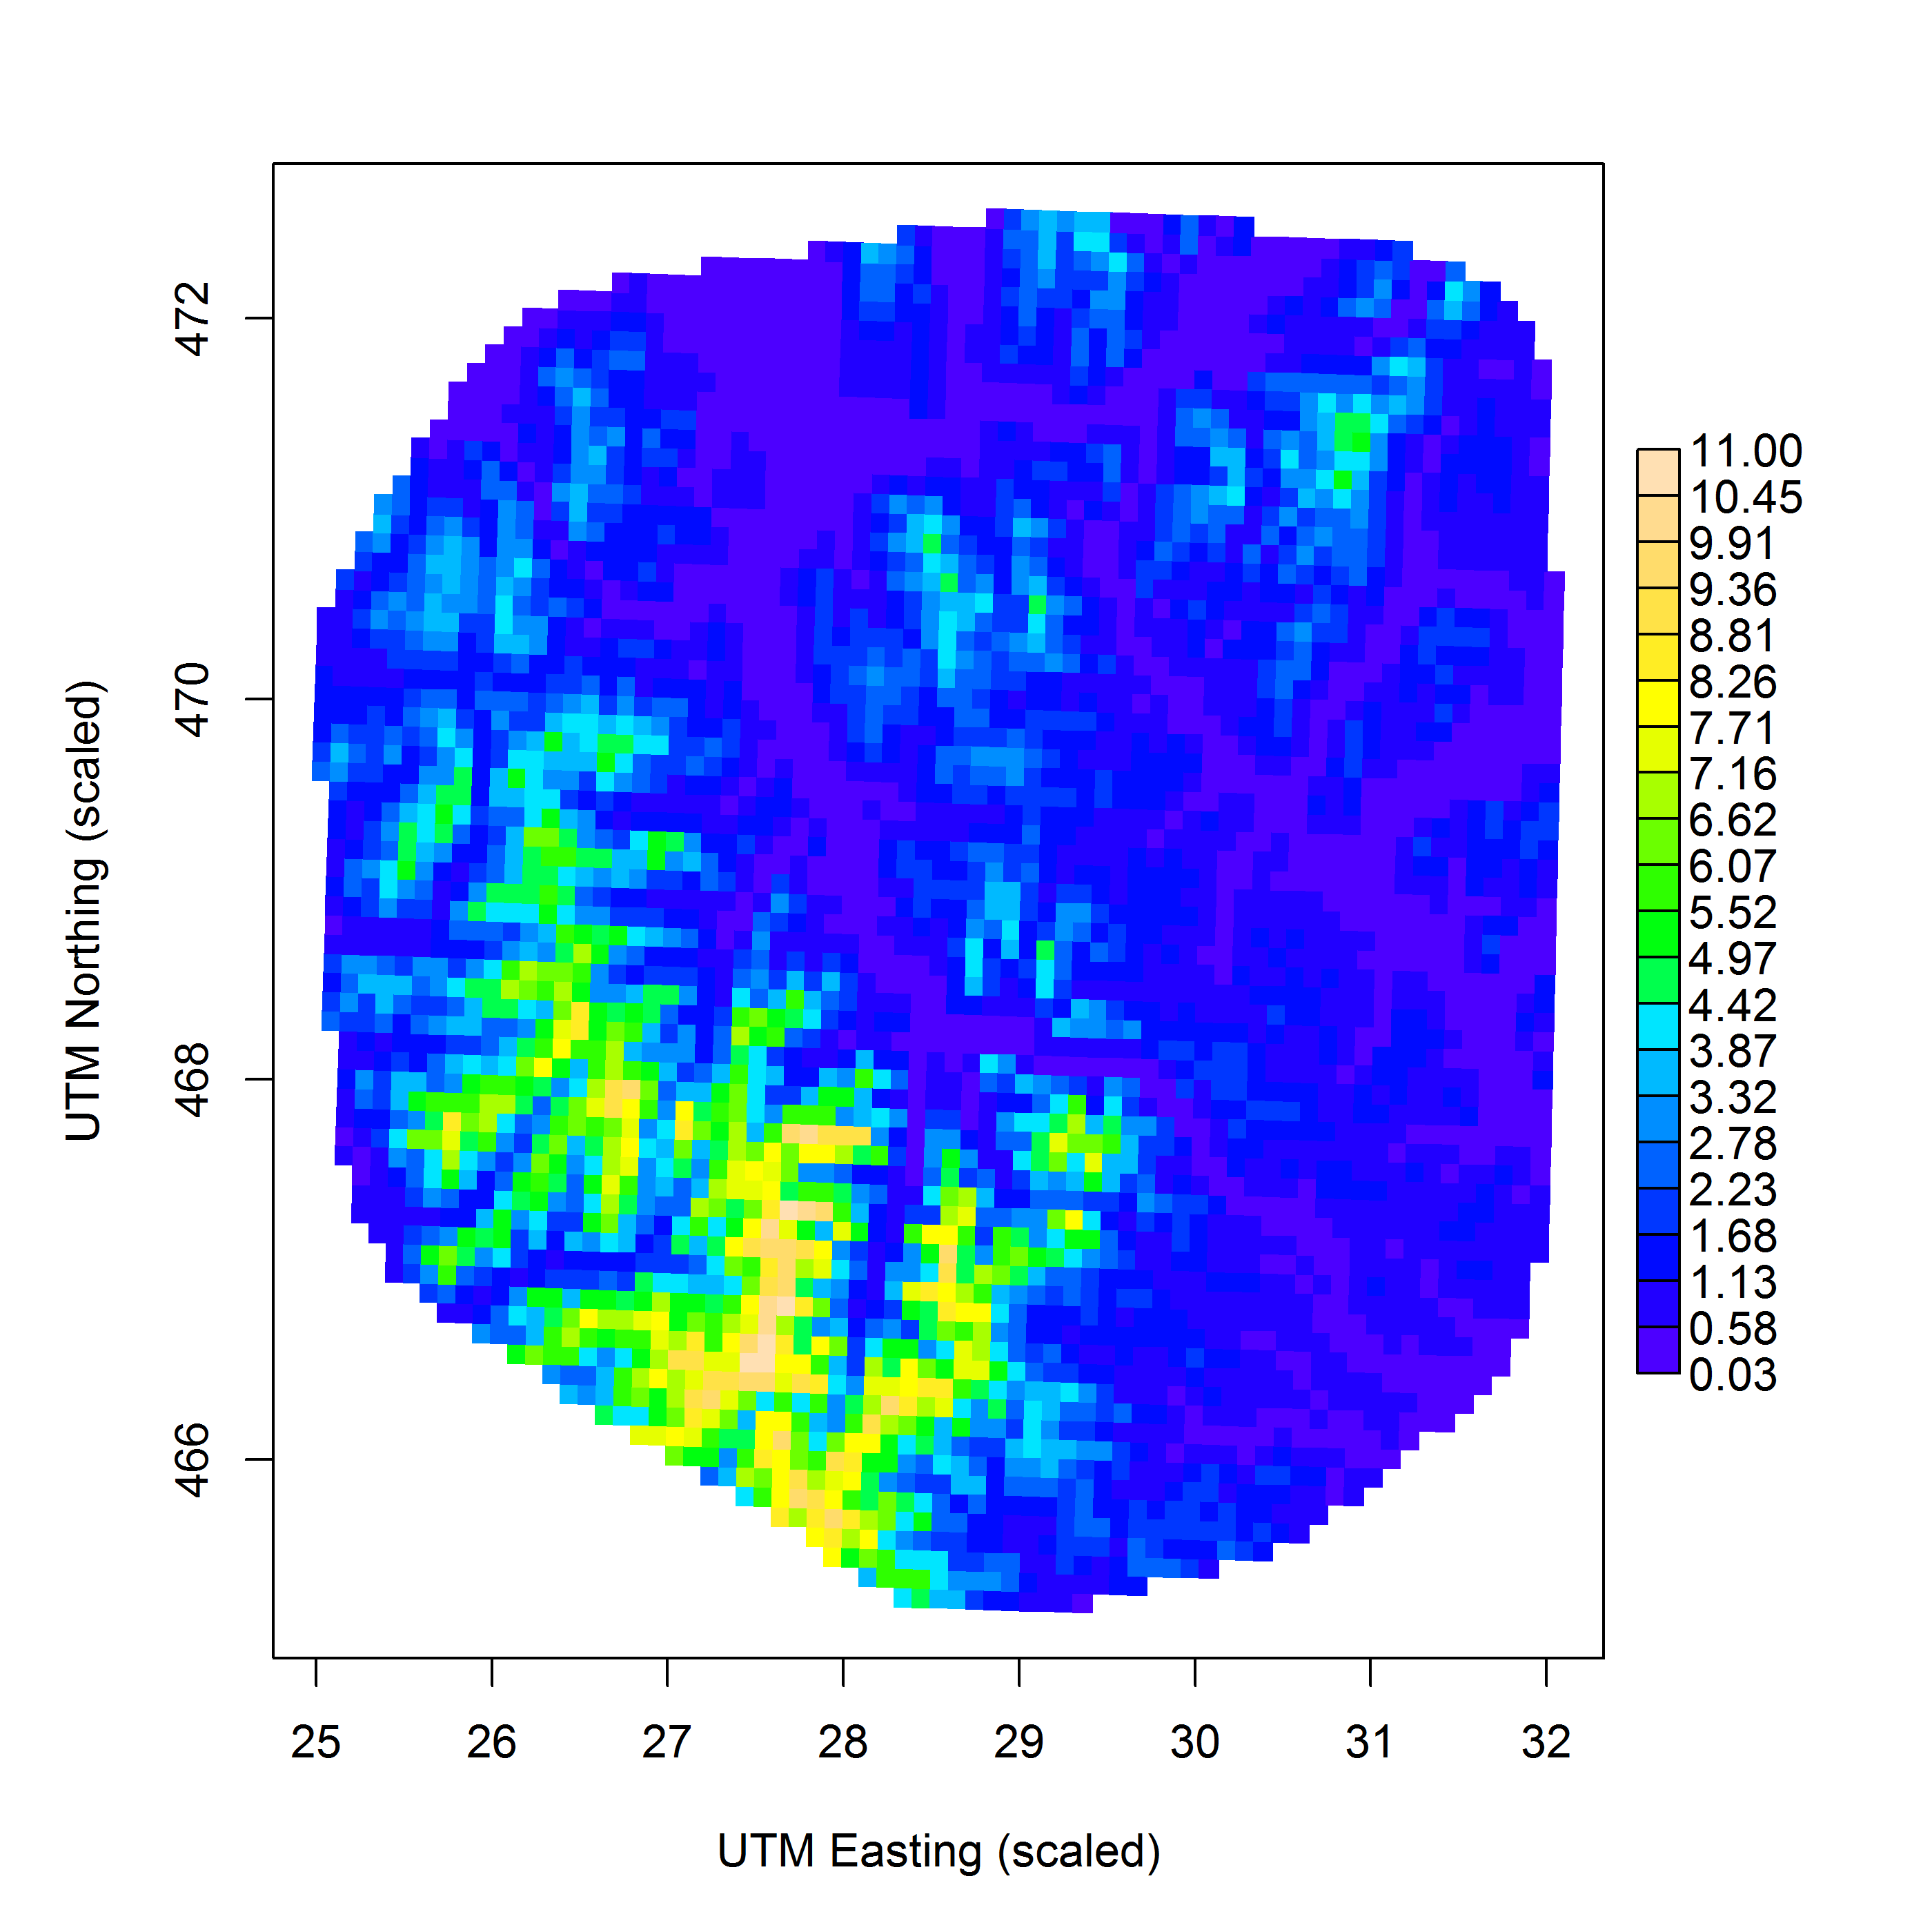
\includegraphics[width=3.25in,height=3.25in]{Ch13-RSF/figs/density2.png}
\caption{Predicted density of black bears (per 100 km$^2$) in
  southwestern  New York study
  area.
}
\label{fig.density}
\end{figure}


\begin{figure}
\centering
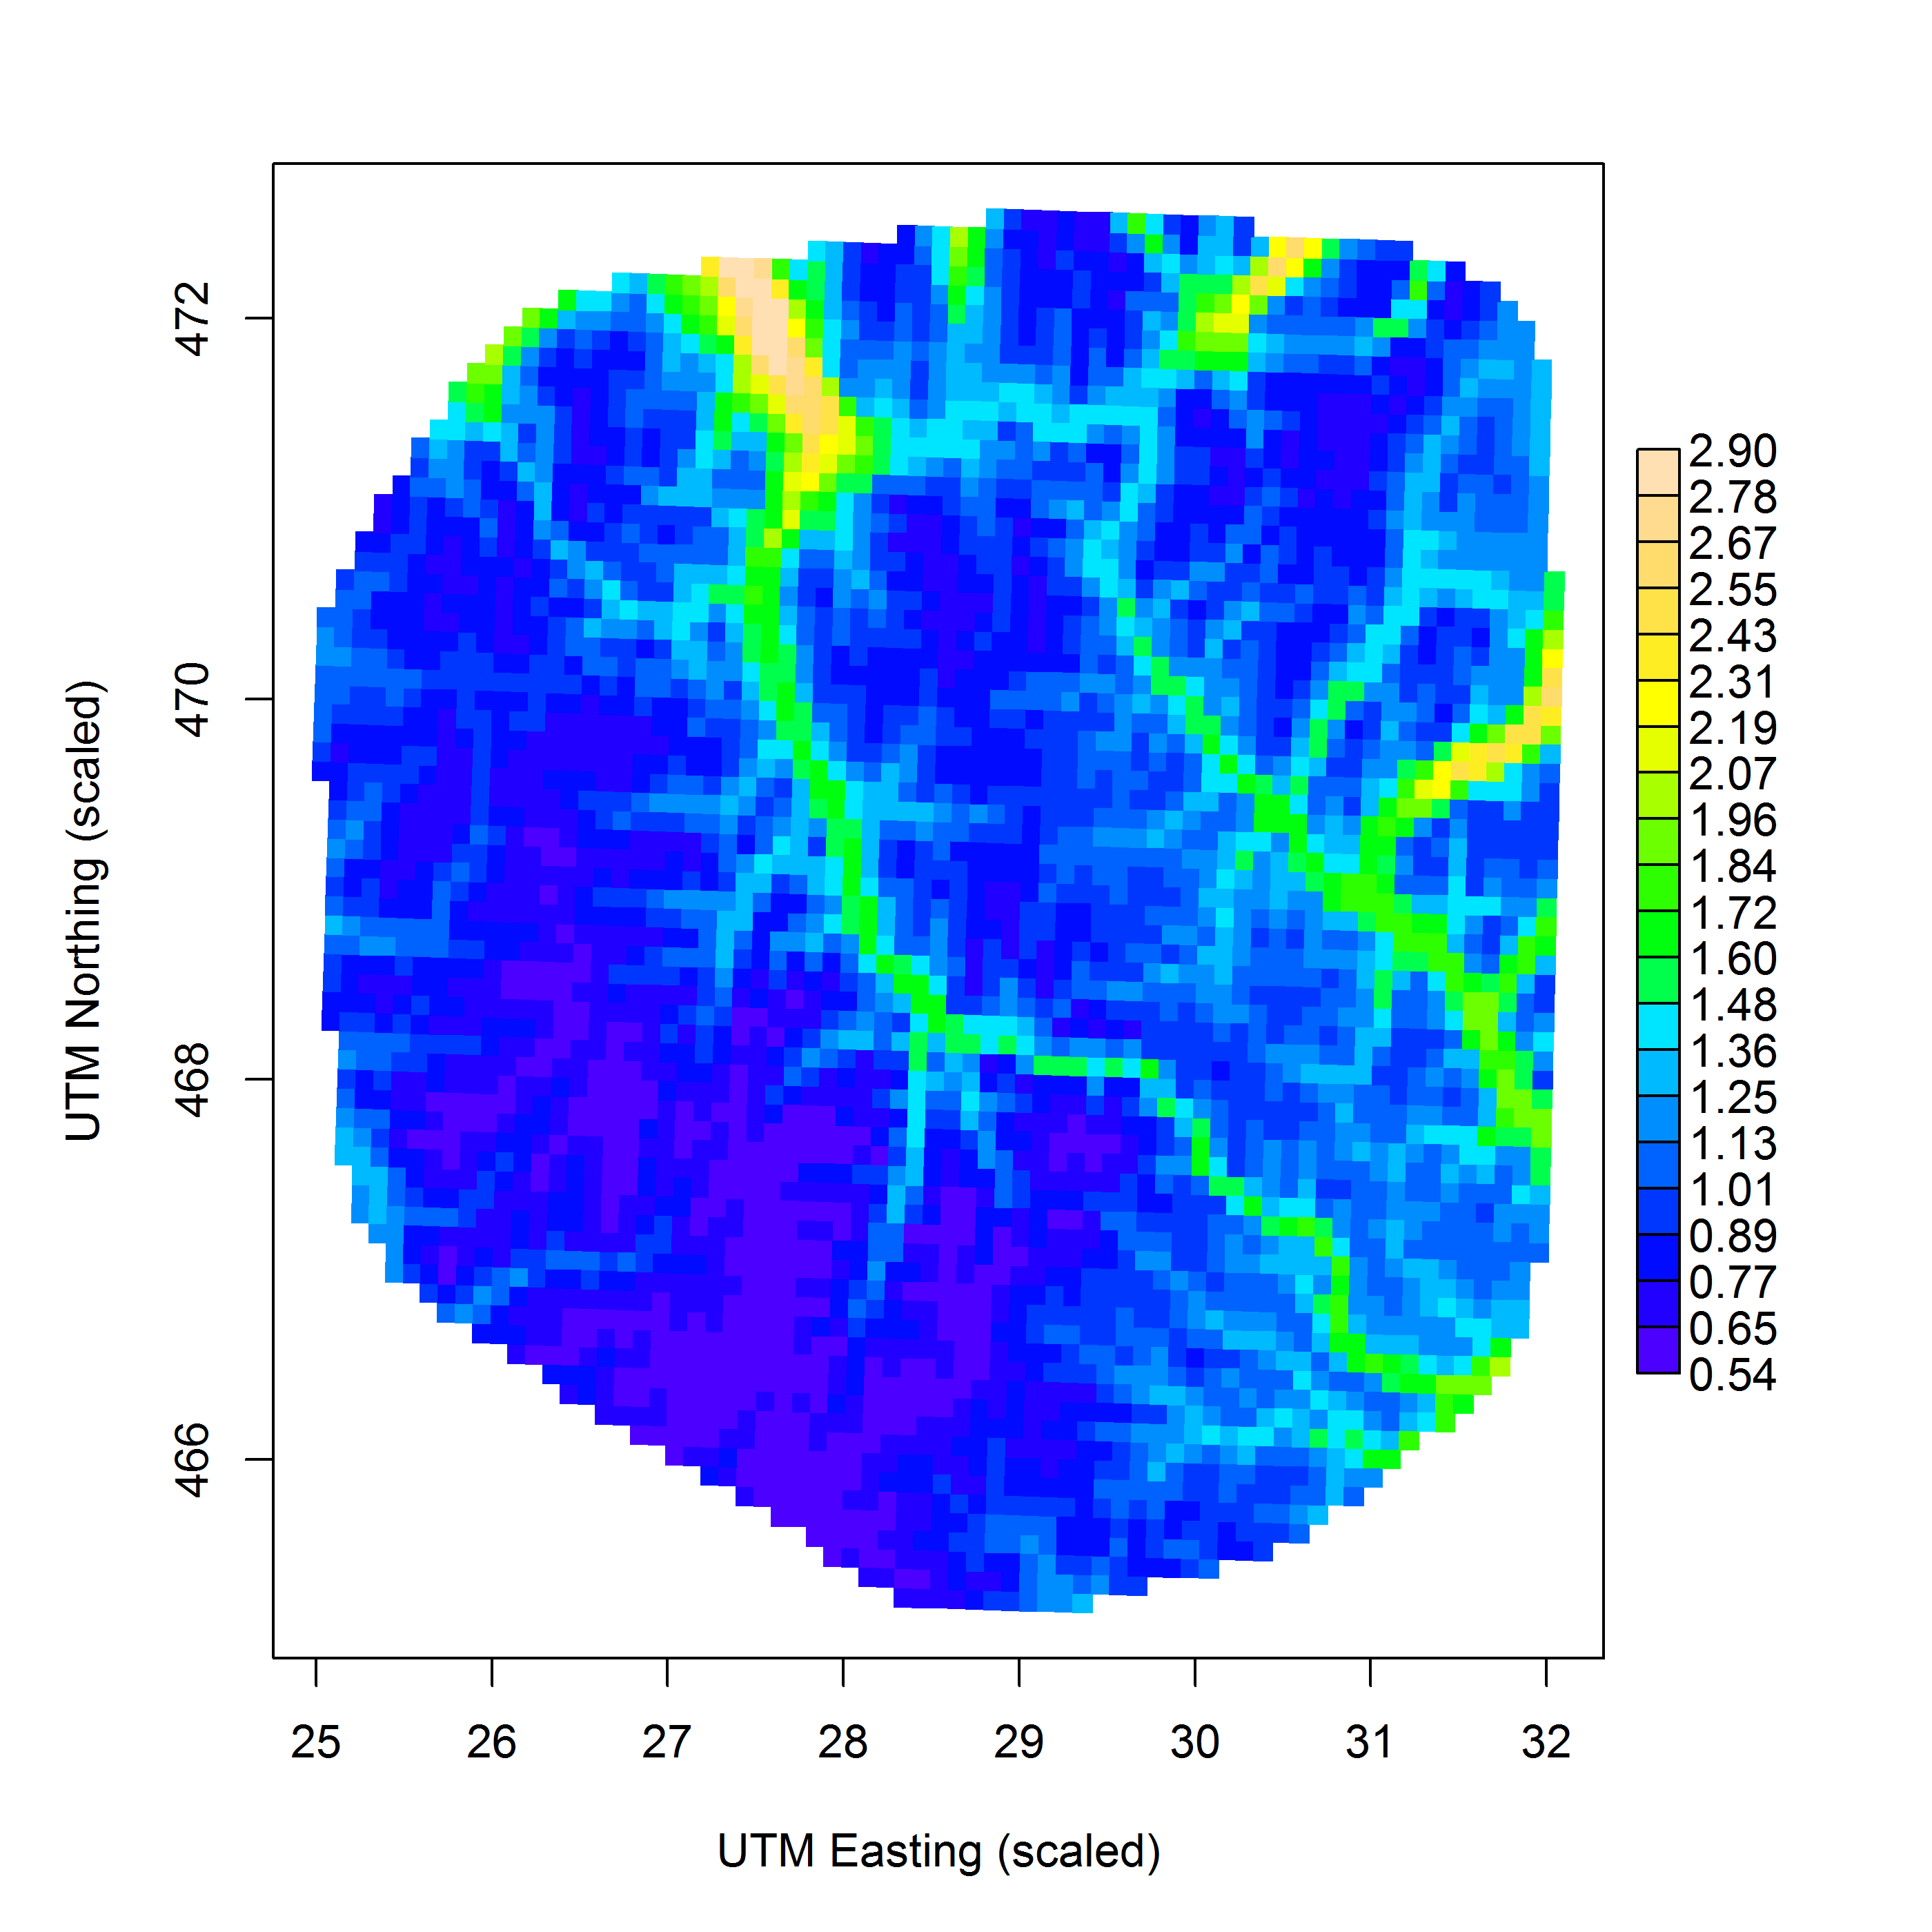
\includegraphics[width=3.25in,height=3.25in]{Ch13-RSF/figs/spaceusage2.png}
\caption{Relative probability of use of pixel ${\bf x}$ compared to a pixel
  of mean elevation, at a constant distance from the activity center.
}
\label{fig.spaceusage}
\end{figure}



\section{Simulation Study}

Using the simulated landscape shown in Fig. \ref{rsf.fig.habitat},
\citep{royle_etal:2012mee} presented results of a simulation study
considering populations of $N=100$ and $N=200$ individuals exposed to
encounter by a 
 $7 \times 7$ array of trapping devices,
% was
%located on the the integer coordinates $(u*5,v*5)$ for $u,v =
%1,2,3,4,5,6,7$ and sampling was conducted for
with $K=10$ sampling occasions, using 
%XX RS: I would put the details back in; maybe not the integer coordinates, but the array and K for sure XXX
%% Andy sez: ok, done. 
the Gaussian hazard model
(Eq. \ref{rsf.eq.cloglog})
with 
\[
\log(\lambda_{ij}) = -2  -\frac{1}{2\sigma^{2}} d_{ij}^{2} + 1 \times C({\bf x}_{j}).
\]
where $\sigma =2$.
In the absence of selection (omitting the covariate $C({\bf x})$),
this model corresponds to a bivariate normal model of space use, 
with standard deviation 2 (Sec. \ref{scr0.sec.implied}).

Using this model, \citet{royle_etal:2012mee} looked at the effect of
misspecification of the resource selection model with an ordinary
model SCR0 (i.e. no habitat covariates affecting the trap encounter model), and the peformance of the MLEs, under SCR+telemetry
designs having 2, 4, 8, 12, and 16 telemetered individuals (with 20
independent telemetry fixes {\it per} individual). 
\citet{royle_etal:2012mee} fitted 3 models: (i) the SCR only model, in which the telemetry
data were not used; (ii) the integrated SCR/RSF model which combined
all of the data for jointly estimating model parameters; and (iii) the
RSF only model which just used the telemetry data alone (and therefore the parameters
$\alpha_{0}$ and $N$ are not estimable).  An abbreviated
version of the results from \citet{royle_etal:2012mee} is summarized
in Table \ref{rsf.tab.sims} below. We provide an {\bf R} script (see \mbox{\tt
  ?RSFsim}) that can be modified for further analysis and exploration.

One thing we see is a pretty dramatic negative
 bias in estimating $N$ if the
 model SCR0 is fitted (interestingly, there is much less bias in
estimating $\sigma$).  Overall, though, when either the SCR model with
covariate or the joint SCR+RSF model is fitted, the MLEs exhibit
little bias for the parameter values simulated here. In terms of RMSE,
there is only a slight $\approx$ 5-10\% reduction in RMSE of the
estimator of $N$ when we have at least 2 telemetered individuals.
% This makes
%sense because we nail down the parameters and still don't know where
%guys are, and get info about mean $p$, i.e. $\alpha_{0}$, only from the
%SCR data. 
%XXX RS: the previous sentence needs some rewording; it's unclear which parameters we nail and under what scenario XXX
Thus estimating $N$ benefits only slightly from the addition
of telemetry data, which is because information about the intercept,
$\alpha_{0}$, comes only from the capture-recapture data.  
However, there is a large improvement in precision (50-60\%) for 
estimating the scale parameter $\sigma$.  While this doesn't
translate much into improved estimation of $N$, it suggests that it
should be relevant to the design of SCR studies for which trap spacing
is one of the main considerations (Chapt. \ref{chapt.design}). In terms of study design these results also
suggest that, perhaps, spatial recaptures are not needed if some
telemetry data are available (in Chapt. \ref{chapt.partialID}, in the context of mark-resight models, we show a case study of raccoons where additional telemetry data allows estimating model parameters in spite of a very low number of spatial recaptures \citep{sollmann_etal:2012ecol}). The resource selection parameter
$\alpha_{2}$ is well-estimated even {\it without} telemetry data. The
fact that parameters of resrouce selection can be estimated from
ordinary capture-recapture data should have considerable practical
relevance in the study of animal populations and landscape
ecology. For the highest sample size of telemetered individuals
($n=16$), the RMSE for estimating this parameter only decreases from
about $0.09$ to $0.07$.



\begin{table}[ht]
\centering
\caption{
  This table summaries the sampling distribution of the MLE of model
  parameters   for models fitted to data generated under a resource selection model.
  The models fitted   include the misspecified model, which is a basic model SCR0 (with no covariate), the SCR model with
  the covariate on encounter probability, and the SCR model including
  the covariate and a sample of telemetered individuals ($n$ is the
  number of individuals telemtered).    Data were simulated with   $N=200$ individuals,
  $\alpha_{2} = 1$ and $\sigma = 2$.
}
\begin{tabular}{ccccccc} \hline \hline 
        &  $\hat{N}$ &RMSE   &  $\hat{\alpha}_{2}$ &RMSE  &        $\hat{\sigma}$ & RMSE    \\ \hline
n=2     &       &       &       &      &        &         \\
SCR+C(x)& 199.11&  14.28&  0.99 &  0.09&   2.00 &  0.090  \\
SCR+RSF & 199.11&  13.80&  0.99 &  0.09&   2.00 &  0.079  \\
SCR0    & 161.48&  39.98&   --  &   -- &   1.84 &  0.180  \\ \hline
n=4   &       &      &        &    &        &          \\
SCR only& 199.67&  13.87&   1.00&   0.09 &  2.00&   0.090 \\
SCR/RSF & 199.65&  13.59&   1.00&   0.09 &  2.00&   0.072\\
SCR0    & 161.32&  40.00&    -- &    --  &  1.83&   0.191\\ \hline
n=8    &       &      &        &    &        &          \\
SCR only& 199.24&  15.49&   0.99&   0.10&   2.01&   0.093 \\
SCR/RSF & 199.55&  14.17&   0.99&   0.08&   2.00&   0.063\\
SCR0    & 161.46&  40.06&    -- &    -- &   1.84&   0.184\\ \hline
n=12    &       &      &        &    &        &          \\
SCR only& 200.41&  15.16&   0.99&   0.10&   2.00&   0.086\\
SCR/RSF & 200.95&  13.04&   1.00&   0.08&   2.00&   0.051\\
SCR0    & 162.40&  38.95&    -- &    -- &   1.84&   0.185\\ \hline
n=16     &       &      &        &    &        &          \\
SCR only &199.16 & 15.62&   1.00 &  0.09&   2.00&   0.095 \\
SCR/RSF  &199.63 & 13.38&   1.00 &  0.07&   2.00&   0.052\\
SCR0     &160.93 & 40.44&    --  &   -- &   1.84&   0.190\\ \hline
\end{tabular}
\label{rsf.tab.sims}
\end{table}





























\begin{comment}
N=100, 300 iters each, mean SCR only N: 99.418     N=200, 500 iters. Mean SCR only N = 199.712
n=2          Nhat RMSE  ahat RMSE  sighat  RMSE    Nhat RMSE  ahat RMSE  sighat  RMSE
SCR only:   99.73  9.97  0.99  0.14  2.00  0.124  198.85  14.24   0.99   0.10   2.00   0.091
SCR/RSF:    99.94  9.54  0.99  0.12  2.00  0.097  199.37  12.80   0.99   0.09   2.00   0.078
sbar        98.89  9.50  0.93  0.14  1.97  0.100  197.87  13.94   0.96   0.10   1.99   0.080
RSF only     --    --    1.03  0.33  2.00  0.160    --      --    1.04   0.33   1.99   0.169
n=4
SCR only    99.10  9.83  0.99  0.13  2.00  0.127  200.06  15.34   1.00   0.09   2.00   0.092
SCR/RSF     99.17  9.47  0.99  0.11  2.00  0.086  200.25  14.36   1.00   0.08   2.01   0.073
sbar        97.43  9.68  0.89  0.16  1.97  0.090  198.14  14.31   0.94   0.10   1.98   0.075
RSF only     --     --   0.98  0.22  2.00  0.119    --     --     1.02   0.21   2.01   0.122
n=8
SCR only    99.59 10.00  1.00  0.13  2.00  0.130  200.85  14.06   1.00   0.09   2.00   0.087
SCR/RSF     98.90 10.02  0.99  0.10  2.00  0.071  200.29  13.98   1.00   0.08   2.00   0.061
sbar        96.07 10.37  0.84  0.19  1.96  0.078  196.46  14.59   0.90   0.13   1.97   0.069
RSF only     --    --    0.98  0.16  2.01  0.084    --     --     0.99   0.16   2.00   0.084
n=12
SCR only    99.44 10.73  0.98  0.13  2.02  0.128  198.76  14.47   0.99   0.10   2.00   0.091
SCR/RSF     99.96 10.26  1.00  0.09  2.00  0.059  198.72  14.14   1.00   0.08   2.00   0.054
sbar        96.30 10.49  0.82  0.20  1.96  0.071  193.83  15.14   0.87   0.15   1.97   0.063
RSF only     --    --    1.01  0.12  2.00  0.069    --     --     1.01   0.13   2.00   0.069
n=16
SCR only    99.23 10.74  0.99  0.14  2.00  0.128  200.04  14.09   0.99   0.10   2.01   0.088
SCR/RSF     99.20  9.79  1.00  0.09  1.99  0.057  200.25  13.40   1.00   0.07   2.00   0.047
sbar        95.10 10.17  0.80  0.22  1.95  0.075  194.38  14.26   0.85   0.17   1.96   0.059
RSF only     --    --    1.00  0.10  1.99  0.061    --     --     1.00   0.11   2.00   0.055





Results for $N=100$, $N=200$ and $N_{tel}=(2,4,8,12,16)$ are presented
in Table \ref{tab.results1}. We note that the first row of each batch
(labeled ``\mbox{\tt SCR only}'') represent the same estimator and data
configuration. These replicate runs of the SCR-only situation give us
an idea of the inherent Monte Carlo (MC) error in these simulations, which is
roughly about 0.25 and 0.89 on the $N$ scale for the $N=100$ and
$N=200$ cases, respectively.  The mean $N$ for the SCR-only
estimator across all 5 simulations for $N=100$ was
$\mbox{mean}(\hat{N}) = 99.418$, an empirical bias of $0.6\%$. For
$N=200$, the estimated $N$ across all 5 simulations (5 levels of
$N_{tel}$) was $\mbox{mean}(\hat{N}) = 199.712$, an empirical bias of
about $0.15\%$, within the Monte Carlo error of the true value of $N=200$.  The
results suggests a very small bias of $< 1\%$ in the MLE of $N$ for
both the  SCR-only and combined SCR/RSF estimators.  In practice, we
expect a small amount of bias in MLEs as likelihood theory only
guarantees asymptotic unbiasedness.


In terms of RMSE for estimating $N$, we see that (Table
\ref{tab.results1}), generally, there is about a 5\% reduction in RMSE
when we have at least 2 telemetered individuals. And, although there
is a lot of MC error in the RMSE quantities, it might be as much as a
10\% reduction as the sample size of captured individuals increases
under the higher $N=200$ setting. This incremental improvement in RMSE
of $\hat{N}$
makes sense because, while the
telemetry provides considerable information about the structural
parameters of the model, it provides no information about mean $p$,
i.e. $\alpha_{0}$, which comes only from the SCR data. Thus estimating
$N$ benefits only slightly from the addition of telemetry data.


The MLE of the RSF parameter $\alpha_{2}$ exhibits negligible or no
bias under {\it both} the SCR only and SCR/RSF estimators. It is
well-estimated from SCR data alone and even better than RSF data alone
(in terms of RMSE) until we have more than 200 or so telemetry
observations\footnote{This may appear pardoxical, but the SCR study is
  generating more spatial locations of individuals than the telemetry
  study based on 2 or 4 individuals}.  The biggest improvement from the use of telemetry data
comes in estimating the parameter $\sigma$. We see that $\hat{\sigma}$
is effectively unbiased, and there is a very large improvement in RMSE
of $\hat{\sigma}$, perhaps as much as 50-60\% in some cases, when the
telemetry data are used in the combined estimator (that does not
translate much into improvements in estimating $N$ as we saw
previously).  Improvement due to adding telemetry data diminishes as
the expected sample sizes increases, and so telemetry data does less
to improve the precision of $\hat{\sigma}$ and $\hat{\alpha}_{2}$ for
$N=200$ than for $N=100$. This is because the SCR data alone are
informative about both of those parameters.


The results as they concern likelihood estimation of $N$ suggest that
there is not a substantial benefit to having telemetry
data. Estimators ``SCR only'' and ``SCR/RSF'' both appear
approximately unbiased for $N=100$ and $N=200$, and for any sample
size of telemetered individuals. The RMSE is only 5-10\% improved with
the addition of telemetry information.  However, we find that there is
substantial bias in $\hat{N}$ if we use the {\it misspecified} model
that contains no resource selection component. That is, if we leave the
covariate $z({\bf x})$ out of the model and incorrectly fit a model
with a symmetric and spatially constant encounter model, we see about
20\% bias in the estimates of $N$ in our limited simulation study
(Table \ref{tab.bias}). As such, accounting for resource
selection is important, even though, when accounted for, telemetry
data only improves the estimator incrementally.
In addition, we find that the importance of telemetry data is
relatively more important for smaller sample sizes. We carried-out one
simulation study for the $N=100$ case, but with lower average encounter
probabilities, setting $\alpha_{0}=-3$. This produces
relatively smaller data sets with  $E[n] = 37$.
There are some important features evident from
the results depicted in Table \ref{tab.lowp}.
 First, as a result of the small samples, the MLE of $N$ is
biased for both SCR only and SCR/RSF estimators, although less biased
for the SCR/RSF estimator than for SCR only. The persistent bias in
$\hat{N}$ for both models results from the information about
$\alpha_{0}$ coming only from SCR data, and that estimator itself is
intrinsically biased in small samples.  Conversely, the estimator of
$\alpha_{2}$, the RSF parameter, appears unbiased for all 3 estimators
(SCR only, SCR/RSF and RSF only), as does the estimator of $\sigma$.
We see relatively larger improvements in RMSE (compared with Table
\ref{tab.results1}) of $\hat{N}$, and those improvements
increase substantially as $N_{tel}$ increases.
\end{comment}


\section{Relevance and Relaxation of Assumptions}


In constructing the combined likelihood for RSF and SCR data, we
assumed the data from capture-recapture and telemetry studies were
independent of one another. This implies that whether or not an
individual enters into one of the data sets has no effect on whether
it enters into the other data set.  We cannot foresee situations in
which violation of this assumption should be problematic or invalidate
the estimator under the independence assumption.  In some cases it
might so happen that some individuals appear in {\it both} the RSF and
SCR data sets. In this case, ignoring that information should entail
only an incremental decrease in precision because a slight bit of
information about an individuals activity center is disregarded.
\begin{comment}
If
individuals that have telemetry instructments can also be encountered
in traps (and properly identified), then it would be possible to
modify the combined likelihood so that the individual activity centers
is preserved across both hunks of the likelihood.  In such cases where
we can match some individuals between the two samples, regarding them
as independent should only entail a minor loss of efficiency because
we are disregarding more precise information on a small number of
activity centers. Moreover, we believe, it is unlikely in practice to
expect the two samples to be completely reconcilable and that the
independence formulation is the most generally realistic.
\end{comment}

 Our model pretends that we do not know anything
about the telemetered individuals in terms of their encounter history
in traps. In principle it should not be difficult to admit a formal
reconciliation of individuals between the two lists. In that case, we
just combine the two conditional likelihoods before we integrate ${\bf
  s}$ from the conditional likelihood. This would be almost trivial to
do if {\it all} individuals were reconcilable (or none, as in the case
we have covered here). But, in general, we think you will often have
an intermediate case, i.e., either none will be or at most a subset
of telemetered guys will be known and there will be some individuals
of unknown mark status. 
In that case, basically a type of marking uncertainty or
misclassification, is clearly more difficult to deal with 
(see
Chapt. \ref{chapt.partialID} for some additional context).

We developed the model in a discrete landscape which regarded
potential trap
locations and the covariate $C({\bf x})$ as being defined on the same
set of points. In practice, trap locations may be chosen
independent of the definition of the raster and this does not pose any
challenge or novelty to the model as it stands. In that
case, the covariate(s) need to be defined at each trap location.
The model should be applicable also to covariates that are naturally
continuous (e.g., distance-based covariates) although, in pratice, it
will usually be sufficient to work with a discrete representation of
such covariates.

The multinomial RSF model for telemetry data assumes independent
observations of resource selection.  This would certaintly be
reasonable if telemetry fixes are made far apart in time (or thinned).
However, as noted by \citet{royle_etal:2012mee}, the independence
assumption is {\it not} an assumption of spatially independent
movement outcomes in geographic space.  Active resource selection
should probably lead to the appearance of spatially dependent
outcomes, regardless of how far apart in time the telemetry locations
are.  Even if resource selection observations are dependent, use of
the independence model probably yields unbiased estimators while
under-stating the variance.  Development of integrated SCR+RSF models
that accommodate more general models of movement is needed.




\section{Summary and Outlook}


How animals use space is of fundamental interest to ecologists and is
important in the conservation and management of many
species. Investigating space use is normally done using telemetry and
models referred to as resource selection functions
\citep{manly_etal:2002} but in all of human %very dramatic here!
history, animal resource selection has {\it never} been studied using
capture-recapture models. Instead, essentially all applications of SCR
models have focused on density estimation.  It is intuitive, however,
that space usage should affect encounter probability and thus it
should be highly relevant to density estimation in SCR applications,
and, vice versa, SCR applications should yield data relevant to
resource selection questions. The development in this chapter shows
clearly that these two ideas can be unified within the SCR
methodological framework so that classical notions of resource
selection modeling can be addresssed simultaneous to modeling of
animal density. What we find is that if animal resource selection is
occurring, this can be modeled as covariate on encounter probability,
with or without the availability of auxiliary telemetry data. If
telemetry data do exist, we can estimate parameters jointly by
cominbing the two likelihood components -- that of the SCR data and
that of the telemetry data.

%%% one idea is to use these models to account for sampling along
%%% trails.
%%% define z(x) = trail density or average distance to trail

Active resource selection by individuals induces a type of
heterogeneous encounter probability, and this induces (possibly
severe) bias in the estimated population size for a state-space when
default symmetric encounter probability models are used.  As such, it
is important to account for space usage when relevant covariates are
known to influence space use patterns.  Aside from properly modeling
this selection-induced heterogeneity, integration of RSF data from
telemetry with SCR models achieves a number of useful advances: First,
it leads to an improvement in our ability to estimate density, and
also an improvement in our ability to estimate parameters of the RSF
function.  As many animal population studies have auxiliary telemetry
information, the incorporation of such information into SCR studies
has broad applicability to many studies.  It seems possible even to
estimate density now, with no spatial recaptures, provided telemetry
data are available.  Secondly, the integrated model allows for the
estimation of RSF model parameters directly from SCR data {\it alone}.
This establishes clearly that SCR models {\it are} explicit models of
space usage. In our view, this greatly broadens the utility and
importance of capture-recapture studies beyond their primary
historical use of estimating density or population size. Finally, we
note that telemetry information provide direct information about the
home range shape parameter, $\sigma$ in our analyses above, and its
estimation is greatly improved with even moderate amounts of telemetry
data (see also \citet{sollmann_etal:2012ecol} and
\citet{sollmann_etal:inprepjapplecol}.  This should have some
consequences in terms of the design of capture-recapture studies
(Chapt. \ref{chapt.design}), especially as it relates to trap spacing.

Simultaneously conductingt telemetry studies with capture-recapture is
extremely common in field studies of animal populations. However, the
simultaneous, integrated analysis of the two sources of data has not
been done.  The new class of integrated SCR/RSF models based on the
\citet{royle_etal:2012mee} model allows researchers to model how the
landscape and habitat influence the movement and space use of
individuals around their home range, using non-invasively collected
capture-recapture data that can be augmented with telemetry data.
This should improve our ability to understand, and study, aspects of
space usage and it might, ultimately, aid in addressing
conservation-related problems such as reserve or corridor design. This
development should greatly expand the relevance and utility of spatial
capture-recapture beyond its use for density estimation.


































\bibliography{AndyRefs_alphabetized}

\end{document}